\documentclass[a4paper,12pt]{article}

% List of packages and custom commands/environments
\usepackage{amsmath,amssymb,amscd}
\usepackage[hidelinks]{hyperref}
\usepackage{dirtree}
\usepackage{tikz}
\usetikzlibrary{calc}
\usepackage{graphicx}
% \usepackage{subfig}
\usepackage{comment}
\usepackage{mathtools}
\usepackage{amsmath}
\usepackage{braket}
\usepackage{multirow}
%\usepackage[inline]{showlabels}
\usepackage{adjustbox}
\usepackage{caption}
\usepackage{subcaption}
\captionsetup{font=footnotesize}
\usepackage[a4paper,margin=2cm, marginparwidth=2cm]{geometry}
\usepackage{float}
\providecommand{\href}[2]{\code{#2}}
\providecommand{\url}[1]{\code{#1}}
\usepackage{bm}
\usepackage[a4paper,margin=2cm, marginparwidth=2cm]{geometry}

\usepackage{adjustbox}


\newcommand{\code}[1]{\mbox{%
        \ttfamily
        \tikz \node[anchor=base,fill=black!12]{#1};%
    }}

    \begin{document}
    \pagenumbering{arabic}
    \newgeometry{left = 1.75cm, right = 1.75cm, top = 1.75cm, bottom = 2cm}
    
    \vspace*{3cm}
    
    \begin{center}
     {\Large MPhil Data Intensive Science}  \\ [3pt]
     {\Large University of Cambridge}  \\ [3pt]
     
     \vspace*{1cm}
     \hrulefill
     \vspace*{0.75cm}
     
     {\LARGE \textbf{AstroCLIP: Cross-Modal Pre-training for Astronomical Foundation Models}} \\ [6pt]
     \large \textbf{Data Analysis Project} \\ [6pt]
     \vspace*{0.05cm}
     \hrulefill
     \vspace*{1.5cm}

     % Add the university logo here
    
\includegraphics[width=0.3\textwidth]{../figures/University_Crest.pdf} 

    \vspace*{1.5cm}
     
     {\Large  Andreas Vrikkis} \\ [6pt]
     {\large  December 14, 2023} \\ [3pt]
     {\large  \LaTeX \hspace{0.03cm} Word count: 6105 } \\ [3pt]
     
     \end{center}   
    
    
    \newpage
    
    \restoregeometry
    
    \newpage
    \begin{center}
        \textbf{ABSTRACT}
    \end{center}
    We present a reproduction and extension of \emph{AstroCLIP}: a model that that facilitates the construction of both galaxy images and spectra into a shared, cross-modal embedding space. This is achieved by fine-tuning a pair of pre-trained single-modal models under a contrastive learning framework. Despite using a smaller spectrum encoder with 2 orders of magnitude fewer parameters than the original work, we achieve similar performance on a range of downstream tasks. We apply the model to extract embeddings from the Dark Energy SPectroscopic Instrument (DESI) images and from its corresponding Legacy Imaging Survey spectra. We demonstrate that the embedding space is effective at (1) accurate semantic similarity search for both in-modality and cross-modality query-retrieval tasks and (2) zero-shot prediction of redshift and stellar mass, achieving a Spearman's rank correlation coefficient $R^2$ of up to 0.87. We then extend the original work by projecting the embeddings space onto a 2D plane using UMAP, and use $k$-Means clustering to formulate clusters of galaxies that are semantically separable in both modalities. Ultimately, our approach demonstrates the ability of AstroCLIP to yield highly informative embeddings that have the emergent property of aligning themselves based on shared semantics and physical galaxy properties.



    \newpage
    
    \tableofcontents
    
    \newpage





%\abstract{The field of astronomy has seen a rapid increase in the volume and complexity of datasets in recent years. The advent of large-scale sky surveys such as the Dark Energy Spectroscopic Instrument (DESI) has resulted in catalogues already containing tens of millions of objects, with others aiming to reach billions in the near future. In this work, we reproduce and extend AstroCLIP - a cross-modal foundation model for galaxies. Specifically, we aim to reproduce the results of version 1 of the AstroCLIP paper of Ref, which we refer to as the `original work'. Our reproduction focuses on the following tasks: Deploy pre-trained single-modal models for galaxy images and spectra for the DESI Legacy Survey. Train a cross-modal model under a contrastive learning framework to align the embeddings of the two modalities in a shared latent space. Reproduce the original work's model performance on a range of downstream tasks, including query retrieval, zero-shot prediction of physical properties. We then extend the original work by further analysing the embedding space structure using clustering algorithms and dimensionality reduction techniques. In doing so, we empirically demonstrate that our cross-modal embeddings can capture semantically meaningful information about galaxies, which are aligned across the two modalities.}


\section{Introduction}

In recent years, the field of astronomy has witnessed a significant surge in the volume and complexity of datasets. Large-scale sky surveys, such as the Dark Energy Spectroscopic Instrument (DESI) \cite{DESI}, have generated catalogues encompassing tens of millions of objects, with future projects targeting the inclusion of billions. As the data volume expands, so does the complexity of the required analysis, necessitating sophisticated methods by researchers to extract meaningful insights. This has led to a growing interest in leveraging data-driven methodologies, particularly machine learning (ML), to aid in the analysis of these extensive astronomical datasets \cite{ivezic2020statistics}.

Despite the diverse range of computational approaches that have been developed, most machine learning (ML) models in astronomy are trained using a \textbf{supervised} learning framework. These models fundamentally depend on the quality and quantity of labelled training data to identify underlying patterns. However, in the field of astronomy, labelled data are often scarce and costly to obtain, often relying on crowd-sourced efforts \cite{willett2013galaxy}. Additionally, supervised models require retraining for each new task, starting with essentially random initialisation of network weights and parameters (random priors). This necessity poses a significant limitation, constraining the scalability and generalisation of these models to novel tasks.

Recently, a new line of research has shifted towards self-supervised learning (SSL) as an alternative approach. These methods learn high-quality, rich \textbf{embeddings}: low-dimensional vector representations that capture semantically meaningful information of objects without the need for labeled training data. This is achieved by training models to perform surrogate tasks, such as identifying corrupted pairs or filling in masked sections of the input data. The extracted embeddings are versatile and can be utilised for various downstream tasks such as similarity searches, clustering, outlier removal. More importantly, they can be used as a `foundation' for further downstream tasks, hence they are often referred to as \textbf{foundation models}.  Approaches of this kind have already revolutionised ML fields, such as computer vision \cite{he2021maskedautoencodersscalablevision} and natural language processing \cite{radford2019language}, where they have demonstrated superior performance compared to their supervised counterparts in zero-shot and few-shot learning tasks.

Numerous SSL approaches have being deployed in the field of observational astronomy, with a notable example being the application of the Momentum Contrastive pretraining strategy (MoCo v2) to galaxy images \cite{stein}. However, these approaches have primarily been limited to embedding objects of a single modality, typically by creating augmented views of the same underlying object. Neverthelss, observational astronomy is inherently multimodal, as the same object can yield a variety of complementary observations. For instance, a galaxy can be observed through both images and spectra, each providing different data structures of the same underlying object. Since these modalities are correlated transformations of the same object, a common embedding space should exist where the representations of these modalities are aligned. Establishing such a universal foundation model for observational astronomy would enable cross-modal tasks such as searches, clustering, and inference

In this work, we reproduce and extend \emph{AstroCLIP} - the first cross-modal foundation model for galaxies. Specifically, we aim to reproduce the results of version 1 of the AstroCLIP paper of Ref\cite{astroclip}, which we refer to as the `original work'. Our reproduction focuses on the following tasks:
%bullet points
\begin{itemize}
    \item Deploy pre-trained single-modal models for galaxy images and spectra for the DESI Legacy Survey \cite{DESI}.
    \item Train a cross-modal model under a contrastive learning framework to align the embeddings of the two modalities in a shared latent space.
    \item Reproduce the original work's model performance on a range of downstream tasks, including query retrieval, zero-shot prediction of physical properties.
\end{itemize}
We then extend the original work by further analysing the embedding space structure using clustering algorithms and dimensionality reduction techniques. In doing so, we empirically demonstrate that our cross-modal embeddings can capture semantically meaningful information about galaxies, which are aligned across the two modalities.

Machine learning (ML) research is currently facing a reproducibility crisis, with many studies proving difficult or even impossible to replicate \cite{kapoor2023leakage}. This often arises due to unpublished data or source code, or due to subtle sensitivities in the training process that are not well-documented. Furthermore, ML code tends to be complex and lacks the standardisation seen in other scientific fields. As the paradigm of predictive modelling using ML gains traction, it is more crucial than ever to undertake reproducibility studies like this one. Here, we discuss the various challenges encountered during the reproduction process and the steps taken to overcome them.



\section{Methodology}
\label{sec:methodology}
%\subsection{Foundational Models}
\subsection{Transfer Learning \& Self-Supervised Learning}
\label{sec:ssl}

Traditional supervised learning frameworks rely heavily on the amount of annotated training data available. When labelled training data are scarce, other datasets can be exploited to improve performance. In \emph{transfer learning} a model is first pre-trained to perform a related secondary task for which we have more (potentially labelled) data \cite{udl}. The resulting model is then adapted to the primary task of interest. This is typically done by removing the final layer(s) of the network and adding new layers (heads) that produce the desired output. Further training is then performed on the primary task. The pre-trained part of the network can be frozen (i.e. its weights are not updated during training) or it can be fine-tuned. The key principle behind this approach is that the pre-trained model has built a good internal representation of the data from the secondary task, which can be useful for the primary task. It can also be seen as a form of sensible weight initialisation for most of the final network.

For transfer learning to be effective, the secondary task should contain a large amount of data. In many cases, however, labelled data are scarce or expensive to obtain, even as secondary tasks. This is where self-supervised learning (SSL) has seen a wide use, in which the secondary task for transfer learning is defined as a  pretext task where the labels are generated from the data itself. In the process, the model learns to extract rich, low-dimensional representations from data without the need for human labelling. The pretext task is often chosen to be an artificial surrogate task on the input data. Recently, numerous such tasks have been developed, including autoregressive prediction of the next word in a sequence \cite{radford2019language}, masked language modelling \cite{devlin2018bert} and contrastive learning \cite{radford2021learning}. Adding to this, pretext tasks can be of different types; for example,  a model can be made to predict the rotation angle of given image \cite{hintonsimpleframework}. These techniques have shown success in generating versatile and informative representations across NLP and computer vision.




\subsection{Contrastive Learning}
\label{sec:contrastive}
Contrastive learning is a SSL technique that produces meaningful representations (embeddings) from an unlabelled dataset. The key idea of contrastive learning is to constrast semantically similar (positive) and dissimilar (negative) pairs of data points, encouraging the representations of positive pairs to be close together in the embedding space, and those of negative pairs to be more orthogonal \cite{chuang2020debiased}. This can be done in a single-modal or multi-modal (cross-modal) setting, where by modality we refer to the type of data input such as images, text, etc. 
In single-modal contrastive learning, a stochastic data augmentation is applied to a given data example to create two correlated views of the same example \cite{hintonsimpleframework}. This is then considered a positive pair, while all other examples are considered negative pairs. %A neural network encoder then extracts embedding vectors from these augmented data examples.

We can extend this to cross-modal contrastive learning by  considering that different observational modalities represent correlated views of the same underlying physical object. This means that a common embedding space should exist where the representations of these modalities can be aligned. As a result, instead of artificially creating the positive and negative pairs through stochastic augmentation, embeddings originating from different modalities of the same underlying object are by construction positive pairs, while all other embeddings are considered negative pairs. We can create these embeddings using separate embedder networks for each modality. These embedders are then trained jointly under a contrastive loss function, whereby positive pairs are projected together in the embedding space, while negative pairs are pushed apart. A prominent example of connecting embeddings across modalities is Contrastive Language-Image Pre-training (CLIP) \cite{radford2021learning}, in which images and text where aligned together in a shared embedding space.   

%The key concept behind the  training objective is that different observational modalities represent correlated transformations of the same underlying physical object, forming a positive pair. By modality we refer to the type of data input such as iamges, text, etc. each requring a different processing technique. This is an extension of the single-modal contrastive learning framework such as SimCLR [cite], which employs stochastic data augmentation to create two views from the underlying image. Instead, we begin with two different modalities in different spaces and map them to a common embedding space, similar to the cross-modal framework connecting language and images in Ref.\cite{crossCLIP}. Under the constrastive loss function, each positive pair is projected together in the embedding space, while negative pairs are pushed apart.  

The cross-modal contrastive learning framework is illustrated in Fig.\ref{fig:contrastive_learning}. Here, $\mathbf{x}_i \in \mathbb{R}^N$ and $\mathbf{y}_i \in \mathbb{R}^M$ represent two modalities of the same underlying object $i$. These modalities are processed through encoder networks $f_{\mathbf{\theta}}: \mathbb{R}^N \rightarrow \mathbb{R}^D$ and $g_{\mathbf{\phi}}: \mathbb{R}^M \rightarrow \mathbb{R}^D$, with $\{\mathbf{\theta}, \mathbf{\phi}\}$ as trainable parameters. The encoders extract representation vectors in a shared embedding space, where contrastive loss is applied. These representation vectors are denoted as $\mathbf{z}^x_i \in \mathbb{R}^D$ and $\mathbf{z}^y_i \in \mathbb{R}^D$, with $D$ being the dimensionality of the embedding space and the superscripts $x$ and $y$ indicating the originating modality. While not necessary, it was shown in Ref.\cite{crossCLIP} that by artificially augmenting the data before passing it through the encoder with a stochastic data augmentation $\mathcal{T}$, the model can learn more robust representations.

\begin{figure}[H]
    \centering
    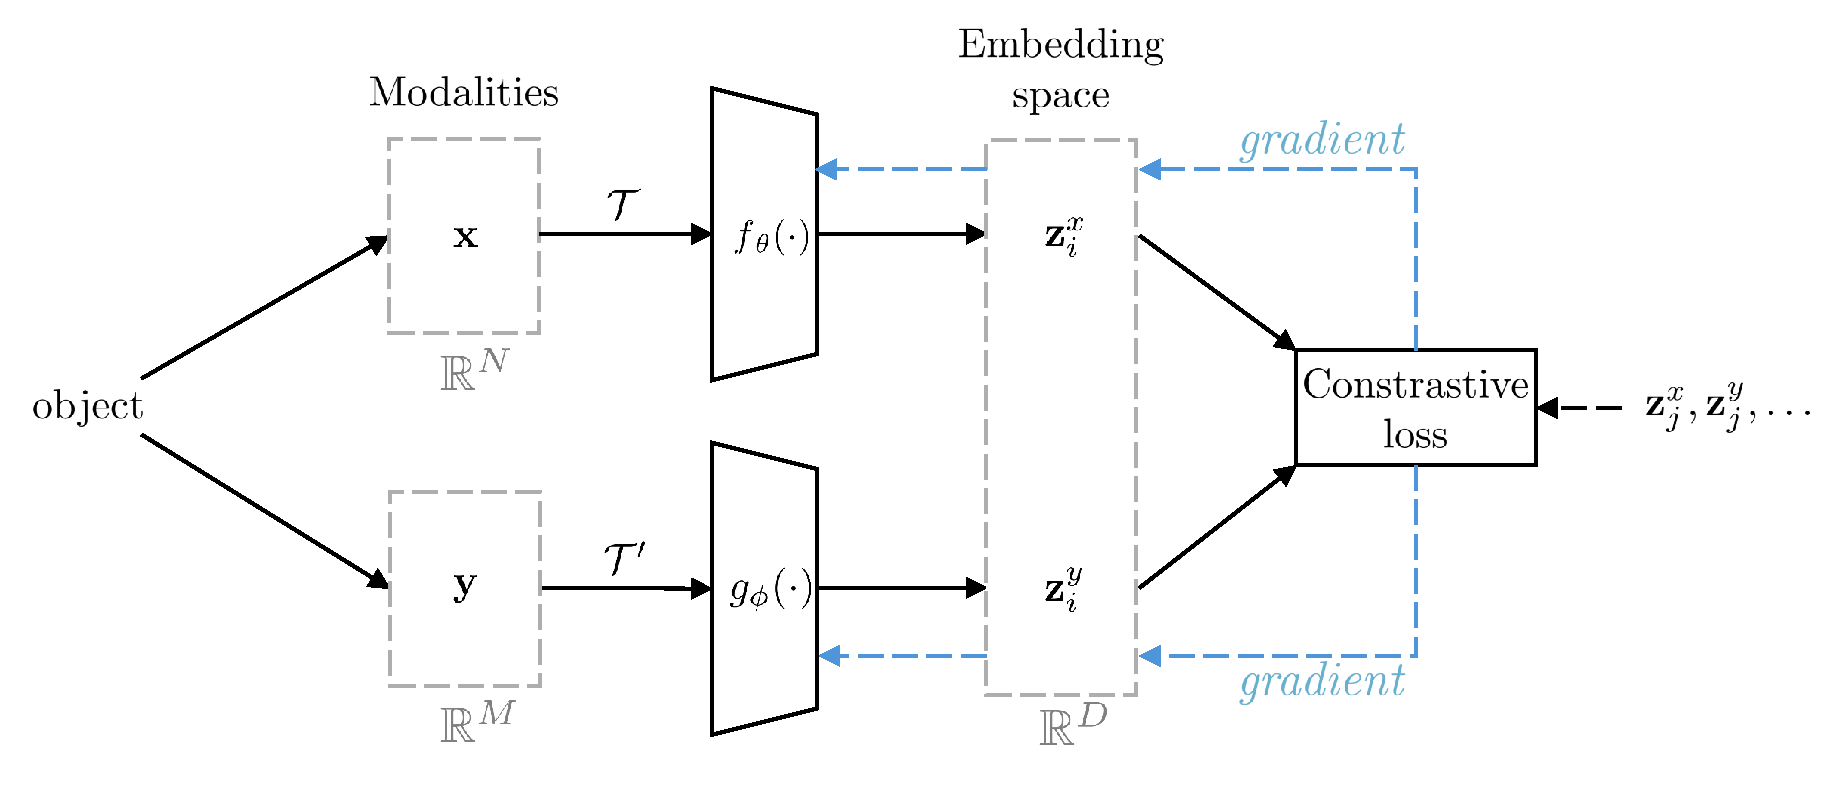
\includegraphics[width=\textwidth]{../figures/diagram_contrastive_learning.pdf}
    \caption{Cross-modal contrastive learning framework. An underlying physical object $j$ is observed in two different modalities, $\mathbf{x_i}\in \mathbb{R^N}$ and $\mathbf{y}_i \in \mathbb{R^M}$. An augmented version of each modality undergoes a transformation $\mathcal{T}, \mathcal{T}'$ and are passed through encoder networks $f_{\theta}, g_{\phi}$ which compress them into representations $\mathbf{z}^x_i, \mathbf{z}^y_i$ in a shared embedding space. The constrastive loss (InfoNCE) is applied to these representations along with the negative pairs denoted by $j$, with the gradients backpropagated to jointly train the encoder networks.}
    \label{fig:contrastive_learning}
\end{figure}


We want this embedding space to maximise the mutual information $I(f_{\theta}(\mathbf{x}),g_\phi{\mathbf{y}})$ between these two representations. However, calculating the mutual information directly is intractable for finite data \cite{mutualinfolimitation}. Instead, we approximate each modality as a noisy transformation of the same underlying object and use an Information Noise-Contrastive Estimation (InfoNCE) loss function \cite{infonce} which maximises a variational bound on the mutual information. The InfoNCE loss is defined as:

\begin{equation}
    \mathcal{L}_{\text{InfoNCE}}(\mathbf{z}^x, \mathbf{z}^y, \tau) = -\frac{1}{K} \sum_{i=1}^{K} \log \frac{\exp\left(S_C(\mathbf{z}^x_i, \mathbf{z}^y_i)/\tau\right)}{\sum_{j}^{K} \exp\left(S_C(\mathbf{z}^x_i, \mathbf{z}^y_j)/\tau\right)}
    \label{eq:infonce}
\end{equation}
where $\mathbf{z}^x_i=f(\mathbf{x}_i)$ and $\mathbf{z}^y_i=g(\mathbf{y}_i)$, $\tau > 0$ denotes a smoothing parameter (referred to as temperature) , $S_C(\mathbf{z}^x_i, \mathbf{z}^y_i)$ is a similarity metric between the two representations, and $j$ represent the indices of negative examples (i.e representations of different objects to object $i$). For the similarity metric in CLIP, we use the cosine similarity between the two representations in the embedding space given by:
\begin{equation}
    S_C(\mathbf{z}^x_i, \mathbf{z}^y_j) = \frac{(\mathbf{z}^x_i)^T \mathbf{z}^y_j}{\|\mathbf{z}^x_i\|^2 \|\mathbf{z}^y_j\|^2}.
    \label{eq:cosine}
\end{equation}
InfoNCE is biased, but it represents a stable, low variance bound on the mutual information that is widely used in contrastive methods \cite{crossCLIP}. Under InfoNCE, points in the embedding space that correspond to the same object are pulled together, while points that correspond to different objects are pushed apart.

Training cross-modal models from scratch under CLIP loss has been shown to often underperform compared to single-modal problems. However, by leveraging transfer learning through the addition of pre-trained single-modal models as initialisation, we can significantly improve performance. This is because the pre-trained models have already learned meaningful representations of the data. In this work, we utilise this approach by deploying pre-trained single-modal models which we appended with a projection head that is trained under the InfoNCE loss. 


\subsection{Embedding Space and Downstream Tasks}
\label{sec:downstream}
 Since the aim of InfoNCE is to bring the vector representations of the same object close together, it has the result of creating a structured embedding space where semantically similar objects are close together, while semantically dissimilar objects are far apart. We can therefore view the embedding space as a multi-dimensional space of point-objects with distances between them having semantic meaning. Following this, the low-dimensional embeddings produced by the encoder networks and aligned under contrastive loss are semantically rich and can be useful for a variety of tasks. We refer to these tasks that come after the training process as \textbf{downstream tasks}. Downstream tasks on the embedding space can include similarity searches or even prediction of physical properties of the objects purely based on the space structure. We refer to the later as \textbf{zero-shot} predictions, as the model has not been trained on the specific task. 
 
 The embedding space can be multi-dimensional, but can be visualised by projecting the representations to a 2D space using dimensionality reduction techniques. One such technique is UMAP (Uniform Manifold Approximation and Projection) \cite{UMAP}, which aims to preserve the global structure and local relationships of data when mapping high-dimensional data to a lower-dimensional space. It does so by constructing a high-dimensional graph representation of the data, which it then optimises to create a low-dimensional projection that maintains as much of the original data's structure as possible.

 The objects in the embedding space can then be grouped into clusters, with each cluster representing a group of semantically similar objects. This can be done both in the original high-dimensional space or in the low-dimensional projection. We can expect that the embeddings of any modality can form meaningful clusters, as during contrastive training each embedding is compared to all other embeddings regardless of modality. Hence, the structure of the embedding space is informed by both modalities and can be used for cross-modal tasks. 



% The low-dimensional, rich representations of the data in the shared embedding space can then be used for a variety of downstream tasks. It has been shown in various contexts that despite the contrived training objective, the embedding space can capture a significant amount of semantic information that often outperform supervised training on zero-shot and few-shot learning tasks. Recall that during constrastive training, the embedding space structures itself such that semantically similar objects are close together, while semantically dissimilar objects are far apart. 
% This means that the positions of the representations in the embedding space can be used to infer semantic relationships between the objects and can be used for downstream tasks. A typical way of visualising the embedding space is to project the representations to a 2D space using dimensionality reduction techniques. 

% UMAP (Uniform Manifold Approximation and Projection) is a dimensionality reduction technique that aims to preserve the global structure and local relationships of data when mapping high-dimensional data to a lower-dimensional space \cite{UMAP}. UMAP constructs a high-dimensional graph representation of the data, which it then optimises to create a low-dimensional projection that maintains as much of the original data's structure as possible. 

% As the embedding space structure is informed by the contrastive loss, the arrangment of the representations holds semantic information. Island structures in the embedding space can be interpreted as clusters of semantically similar objects, while the distance between islands can be used to infer semantic relationships between the clusters.


\section{Implementation}
\label{sec:implementation}
In AstroCLIP, we consider two modalities of galaxies: images and spectra. In essence, we approach the two modalities as filtered, noisy views of the same underlying galaxy. This implies that they should possess a shared latent space in which the embeddings of these cross-modal representations are aligned. To obtain these embeddings, we deploy a pair of models to encode the images and spectra. This process is carried out in two steps:
\begin{enumerate}
    \item We utilise two pre-trained single-modal models, one for images and one for spectra, which were pre-trained using SSL, to enhance our model performance through transfer learning. For the pretrained image embedder, we use a galaxy image encoder from Stein et. al (see Ref.\cite{stein}), which is based on MoCo v2 \cite{mocov2}. For galaxy spectra, we employ the encoder part from the Spender model \cite{spender}.
    \item We append a simple Multilayer Perceptron (MLP) to each of the pre-trained models to compress the representations into a shared $d=128$-dimensional embedding space. We then proceed to train (or fine-tune) both MLP projection heads jointly under InfoNCE loss, to align the embeddings of the two modalities under shared semantics.
\end{enumerate}
We keep the pre-trained encoders frozen during training and only update the MLP heads under InfONCE loss, rather than training the entire model from scratch. This approach is consistent with previous studies showing that employing pre-trained the single-modal models significantly improves performance in cross-modal tasks \cite{crossCLIP}.

It is important to note a deviation from the original work: in the original AstroCLIP (v1) paper, the authors pre-train a transformer model, structured similarly to GPT-2, to embed the spectra \cite{astroclip}. This model is substantially larger than Spender, comprising approximately 43.2M parameters. However, the transformer model is not publicly available, and the authors do not provide details on the pre-training process. Consequently, we opt to use the Spender model based on the recommendation of one of the authors. We provide details of the two models, the data used, and the training process in the following sections.





\subsection{Data}
\label{sec:data}
\subsubsection{DESI Legacy Survey Images}
We use the same data as the original work. For galaxy images, we utilise the DESI Legacy Survey Data Release 9 imaging data from January 2021 \cite{DESI}, as prepared by Stein et al. \cite{stein}. The $g$ and $r$ band data for the northern galactic cap (NGC) were captured by the Beijing-Arizona Sky Survey, while the $z$ band data were obtained from the Mayall Legacy Survey. For the southern galactic cap (SGC), the data were collected by the Dark Energy Camera Legacy Survey (DECaLS). We exclude images identified as stars by the Legacy Survey team and impose a cutoff for $z$-bands above 20. This results in an initial dataset of 41 million (g, r, z) images of size $256 \times 256$, which we centre-crop to $96 \times 96$ for training. The cropping is necessary because the vast majority of galaxies occupy less area than the total image size and often include overlapping regions of the sky.


\subsubsection{DESI Spectra}
To pair the images with spectra, we cross-match the galaxy spectra from the DESI Early Data Release \cite{DESI2023}, which contains spectra observed during the Survey Validation campaign. This cross-matching is performed using the target IDs associated with each galaxy, resulting in a total subset of 197,976 pairs of images and spectra. During the training process, we Z-score normalise each individual spectrum to have zero mean and unit variance. We then split the data into training and validation sets, with 90\% of the data used for training and 10\% for validation.


\subsubsection{Data Catalogue for Downstream Tasks}

%For experiments involving the prediction of physical properties from the embeddings, we further cross-match the image-spectrum pairs with the PRObabilistic Value-Added Bright Galaxy Survery (PROVABGS) catalogue \cite{PROVABGS}. We then specifically extract the estimates of the redshift $Z_{HP}$ and stellar mass ($M_{\star}$) for each galaxy ID that is present in the catalogue. We then perform the same filtering process as the original AstroCLIP paper: we only select enetries for which $M_{\star} > 0$ and mag$_g$,mag$_r$,mag$_z$ $> 0$, removing spurious entries. This yields a total of 105,159 entries, which we split into training and validation using a 90/10 ratio.
For experiments involving the prediction of physical properties from the embeddings, we further cross-match the image-spectrum pairs with the PRObabilistic Value-Added Bright Galaxy Survey (PROVABGS) catalogue \cite{PROVABGS}. Specifically, we extract the estimates of the redshift $Z_{HP}$ and stellar mass ($M_{\star}$) for each galaxy ID present in the cross-matched catalogue. We then perform the same filtering process as outlined in the original AstroCLIP paper: selecting entries where $M_{\star} > 0$ and mag$_g$, mag$_r$, mag$_z$ $> 0$, thereby removing spurious entries. This process yields a total of 105,159 entries, which we split into training and validation sets using a 90/10 ratio.


\subsection{Pre-trained Image Embedder} 
\label{sec:resnet}

\begin{figure}[H]
    \centering
    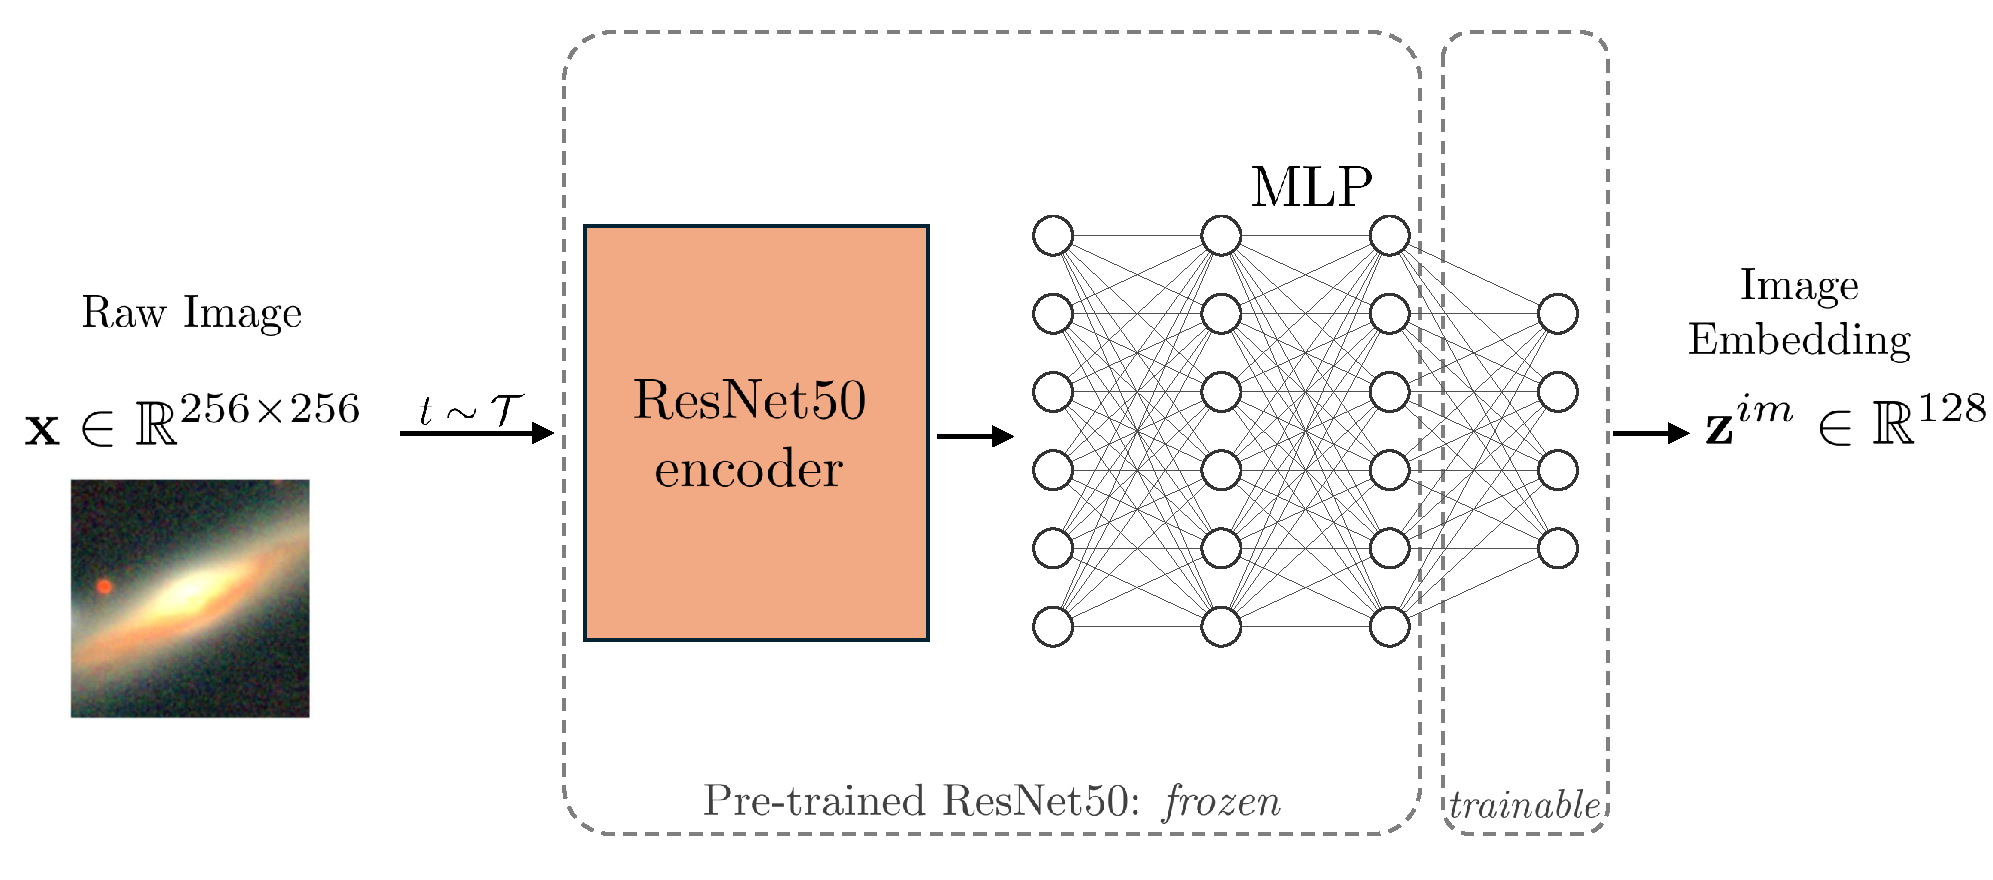
\includegraphics[width=0.9\textwidth]{../figures/diagram_resnet.pdf}
    \caption{Overview of our image embedding procedure. Each raw galaxy image of size $256 \times 256$ undergoes an augmentation and is fed into the ResNet50 based pre-trained image embedder. During our contrastive training phase, we keep all the original weights frozen except the final layer of the MLP. After the training phase, we obtain the image embedding $\mathbf{z}^{\text{im}}$ of vector size $d=128$ that is now in the shared embedding space.}
    \label{fig:resnet}
\end{figure}
The pre-trained image embedder used in this reconstruction was developed by Stein et al. (2021a) \cite{stein}. It is based on the MoCo v2 framework \cite{mocov2}, utilising a ResNet50 backbone as the encoder network. The model was pre-trained on a curated subset of 3.5 million galaxies, sampled uniformly by $z$-band magnitude from the DESI Legacy Survey. The authors employed a single-modal contrastive learning SSL framework, where each image underwent multiple stochastic augmentations to create two views of the same image. These augmentations included galactic extinction, random cropping, random rotation, size scaling, point-spread function blur, jittering, and Gaussian noise addition. The model was then trained using a contrastive loss function to align the representations of the two views in the embedding space. An overview of our image embedding procedure is shown in Fig.\ref{fig:resnet}.

The encoder part of the network is a ResNet50 backbone adapted to extract embeddings from astronomical images. The encoding process begins by passing the images through a series of convolutional blocks, each containing a convolutional layer, followed by batch normalisation, ReLU activation, and max pooling. The core of the network consists of four sequential layers of residual blocks, each containing multiple convolutional layers with batch normalisation and ReLU activations. Some blocks include downsampling layers to adjust the dimensions of the feature maps. The resulting embeddings are then passed through a fully connected network (MLP) with 2048 input features and 2048 output features.

During our cross-modal contrastive training phase, we keep all encoder layers and all except the final MLP layer frozen. We adapt the final fully connected layer to output a $d=128$-dimensional embedding space, allowing the layer's weights and biases to be trainable under the InfoNCE loss. This results in 4.5 million trainable parameters fine-tuned during the training phase. To enhance model performance, we artificially create more positive pairs by applying basic stochastic transformations $t \sim \mathcal{T}$ to the images. These transformations include random rotations, random horizontal and vertical flips, and random Gaussian noise.



% This encoder part of the network is a ResNet50 encoder which consists 50 residul blocks containing a batch normalisation operation, followed by a convolutional layer and GeLU activation functions. They then connect to a 


% It has a total of 28M parameters. 

% We keep all layers frozen during constrastive training, except the last fully connectand use the final fully connected layer as the trainable projection head. This amounts to 4.5M trainable parameters that are finetuned under InfoNCE loss. 


\subsection{Pre-trained Spectrum Embedder}
\label{sec:spender}


\begin{figure}[H]
    \centering
    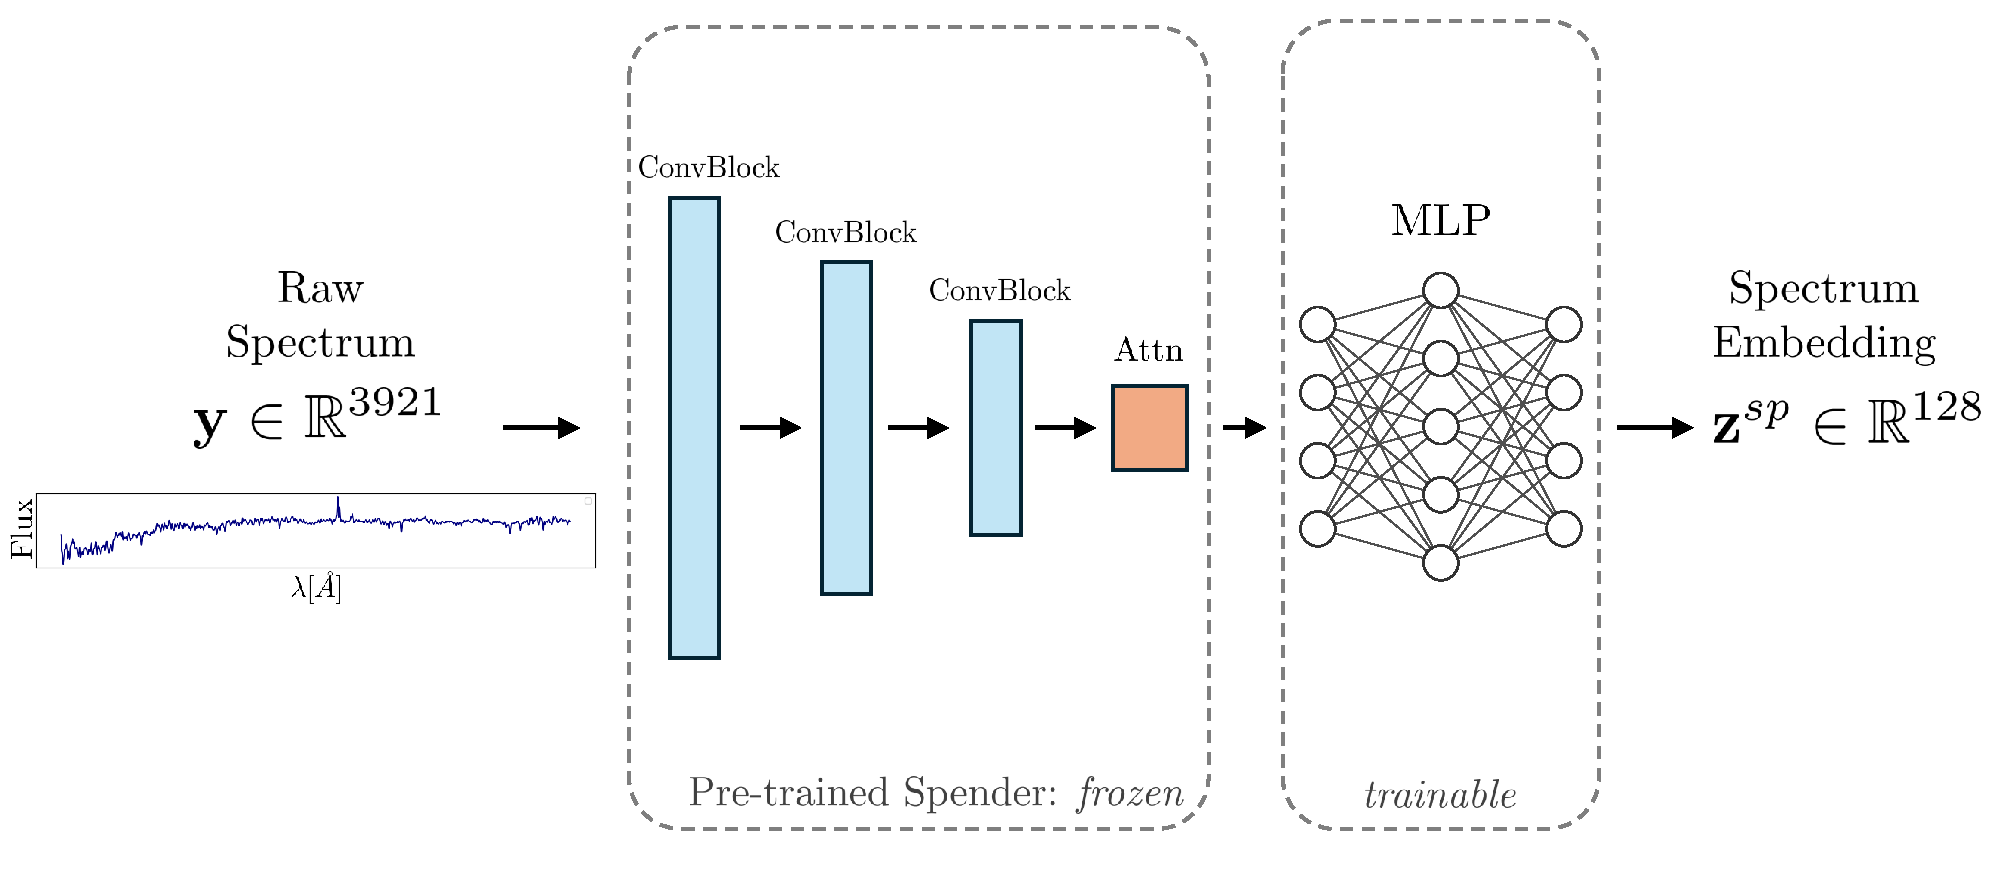
\includegraphics[width=\textwidth]{../figures/diagram_spender_cropped.pdf} % 1.3x text width to extend into the margins
    \caption{Overview of our spectrum embedding procedure. A raw, 1-dimensional galaxy spectrum of size $3921$ is fed through the pre-trained encoder part of the Spender model, the weights of which are kept frozen during the cross-modal contrastive training proces. This consists of three convolutional blocks (ConvBlock) followed by an attention mechanism. The output of the encoder is then passed through a trainable MLP head which copresses the representation into a $d=128$ dimensional vector representation. The final embedding $\mathbf{z}^{\text{sp}}$ is in the shared embedding space.}
    \label{fig:spender}
\end{figure}


We choose to use the Spender model \cite{spender}, an autoencoder network, to extract latent parameters from the observed spectra. The overall spectrum embedder is shown in Fig.\ref{fig:spender}. The encoder part of the network consists of three convolutional blocks (ConvBlocks), each containing a convolutional layer followed by trainable ReLU activation functions and max pooling. The convolutional layers have progressively wider kernel sizes (5, 11, 21), which translates the $M=3921$ spectral components into 512 channels for 72 wavelength segments.  The model then applies attention by splitting the channels into two: $\mathbf{h}$ and $\mathbf{k}$, each of dimension $256 \times 72$. These channels are then combined as follows:


\begin{equation}
    \mathbf{e} = \mathbf{h} \cdot \text{softmax}(\mathbf{k}) \equiv \mathbf{h} \cdot \mathbf{a},
\end{equation}
where the dot product and the softmax are applied on the last dimension, denoting the wavelength. The attention weights in vector $\mathbf{a}$ indicate the presence and location of relevant signals, allowing the corresponding values to be enhanced into the attended features $\mathbf{e}$. This approach efficiently accommodates the apparent shift of spectral features in galaxies at varying redshifts. The attended features are then fed into a series of fully connected layers, compressing the representation into a $s=6$ dimensional latent space. This latent representation is subsequently passed to the decoder part of the network, which reconstructs the original spectrum. As usual in autoencoder networks, it is trained end-to-end with an MSE loss function.

For AstroCLIP, we discard the decoder part of the network and use the convolutional layers and attention mechanism of the encoder. We replace the MLP, which originally compressed the representation into a 6-dimensional latent space, with a new fully connected MLP comprising three hidden layers of sizes [256, 128, 128] and a final output layer of size $d=128$ with ReLU activation functions. This is then trained under the InfoNCE loss function, while the convolutional layers and attention mechanism are kept frozen. These frozen layers retain semantic information about the spectra, which is beneficial through transfer learning. Overall, this results to 230,272 trainable parameters, two orders of magnitude fewer than the original work's spectrum encoder, which totalled 43.2 million parameters \cite{astroclip}.

\subsection{Contrastive Training}
\label{sec:training}
The pre-trained models are used as components of our unified AstroCLIP model. We further train both models jointly under the InfoNCE loss defined in Eq. (\ref{eq:infonce}) using the training set of image-spectrum pairs as obtained in section \ref{sec:data}. Embeddings originating from the same galaxy are considered positive pairs, while all others are considered negative pairs. Before an image is passed through the image embedder, we apply basic augmentations as follows: a fixed crop to the central $96 \times 96$ pixels, random rotation, random horizontal flip, and Gaussian blur. We normalise the embeddings for the similarity metric of Eq. (\ref{eq:cosine}) using the L2 norm.We set the batch size to $K=512$ image-spectrum pairs, as larger batch sizes often correlate with better performance, consistent with the findings of Ref. \cite{radford2021learning}. We train the models using the Adam optimiser \cite{adam} for 80 epochs on a single NVIDIA A100-SXM-80GB GPU on the Cambridge Wilkes3 cluster. We use an adaptable learning rate scheduler that reduces the learning rate by a factor of 2 (chosen by trial and error) if the validation loss does not improve for 5 epochs, using \verb|PyTorch|'s \verb|ReduceLROnPlateau| \cite{LRon}. Similar to results observed in other studies, such as Ref.\cite{gir}, our performance improves when we keep the temperature parameter $\tau = 15.5$ constant rather than allowing it to vary. The cross-modal contrastive training process takes roughly 2 hours to complete.

\subsection{Downstream Tasks}
\label{sec:downstream_tasks}
To demonstrate the capabilities of AstroCLIP's embedding space, we evaluate its performance across a range of tasks for which it was neither explicitly trained nor fine-tuned. Firstly, we embed all galaxy images and spectra in the validation set (obtained as outlined in Section \ref{sec:data}) using our trained AstroCLIP model as follows:

\begin{equation}
    \text{Initial Modality Representation} : \left( \mathbf{x}, \mathbf{y} \right) \xmapsto{\text{AstroCLIP}} \text{Embeddings} : \left( \mathbf{z}^{\text{im}}, \mathbf{z}^{\text{sp}} \right) \in \mathbb{R}^{128}.
\end{equation}
where $\mathbf{x}, \mathbf{y}$ are the raw galaxy images and spectra, and $\mathbf{z}^{\text{im}}, \mathbf{z}^{\text{sp}}$ are the corresponding image and spectrum embeddings. We then normalise both image and spectrum embeddings as:
\begin{equation}
    \mathbf{\bar{z}}^{\text{im}} =  \frac{\mathbf{z}^{\text{im}} }{|| \mathbf{z}^{\text{im}} ||_2}, \quad \mathbf{\bar{z}}^{\text{sp}} =  \frac{\mathbf{z}^{\text{sp}} }{|| \mathbf{z}^{\text{sp}} ||_2}
\end{equation}
and use the normalised galaxy embeddings in a shared, cross-modal latent space to perform the tasks outlined below.


\subsubsection{Query Retrieval}
% We showcase the AstroCLIP's ability to align embeddings of galaxies, we choose a random galaxy from the validation set and retrieve similar galaxies purely based on the embedding space structure. Specifically, we perform the galaxy search using the cosine-similarity (eq.(\ref{eq:cosine})) between the query galaxy $\bar{\mathbf{z}}_q$ and all other galaxies in the validation set. We then rank the galaxies based on the similarity score and display the top 5 most similar galaxies. For instance, to search for galaxy images that are similar to a specific query spectrum $\mathbf{y}_i$, we calculate the cosine similarity between the query spectrum embedding $\mathbf{z}^{\text{sp}}_i$ and the all image embeddings $\{\mathbf{z}^{\text{im}}_{j}\}_{val}$ in the validation set. We denote this similarity score as $S_C(\mathbf{z}^{\text{sp}}_i, \mathbf{z}^{\text{im}}_j)$. The target images with the highest similarity values are then returned. This process requires no additional transformations or alterations.

% This allows us to search the embedding space for both the image and spectrum embeddings, which is unique to this cross-modal framework. We present examples for both \emph{in-modality} $S_{C}(\mathbf{z}^{\text{im}}_q, \mathbf{z}^{\text{im}}_j)$ or $S_{C}(\mathbf{z}^{\text{sp}}_q, \mathbf{z}^{\text{sp}}_j)$, where the query and target embeddings are of the same modality, and \emph{cross-modality} $S_{C}(\mathbf{z}^{\text{im}}_q, \mathbf{z}^{\text{sp}}_j)$ or $S_{C}(\mathbf{z}^{\text{sp}}_q, \mathbf{z}^{\text{im}}_j)$, where the query and target embeddings are of different modalities.

To showcase AstroCLIP's ability to the galaxy embeddings, we randomly select a galaxy from the validation set and retrieve similar galaxies purely based on the embedding space structure. Specifically, we perform the galaxy search using the cosine similarity (Eq. (\ref{eq:cosine})) between the query galaxy $\bar{\mathbf{z}}_q$ and all other galaxies in the validation set. We then rank the galaxies based on the similarity score and display the top 5 most similar galaxies.

For instance, to search for galaxy images similar to a specific query spectrum $\mathbf{y}_q$, we calculate the cosine similarity between the query spectrum embedding $\mathbf{z}^{\text{sp}}_q$ and all image embeddings $\{ \mathbf{z}^{\text{im}}_j \}$ in the validation set. We denote this similarity score as $S_C(\mathbf{z}^{\text{sp}}_q, \mathbf{z}^{\text{im}}_j)$. The target images with the highest similarity values are then returned. This process requires no additional transformations or alterations.

This allows us to search the embedding space for both image and spectrum embeddings, which is unique to this cross-modal framework. We present examples for both \emph{in-modality} $S_{C}(\mathbf{z}^{\text{im}}_q, \mathbf{z}^{\text{im}}j)$ or $S_{C}(\mathbf{z}^{\text{sp}}_q, \mathbf{z}^{\text{sp}}j)$, where the query and target embeddings are of the same modality, and \emph{cross-modality} $S_{C}(\mathbf{z}^{\text{im}}_q, \mathbf{z}^{\text{sp}}j)$ or $S_{C}(\mathbf{z}^{\text{sp}}_q, \mathbf{z}^{\text{im}}_j)$, where the query and target embeddings are of different modalities.





\subsubsection{Zero Shot Prediction of Physical Properties}
To quantify AstroCLIP's inference abilities, we consider the task of predicting the redshift $Z_{HP}$ and stellar mass $M_{\star}$ of galaxies purely from their extracted embeddings. Each embedding has a corresponding redshift and stellar mass value provided by the PROVABGS catalogue. These values are used as the ground truth for the prediction task but were not used in the training process.

We perform a simple $k$-Nearest Neighbour ($k$-NN) regression on the embedded representations to predict the redshift and stellar mass values. $k$-NN regression works by averaging the output values of the $k$-nearest data points to predict the value for a new data point. To that end, we further split the 30,0000 pairs in the validation set into a training set and a held-out set. In $k$-NN regression, `training' means simply storing the image embeddings and their corresponding redshift values. We then use the train set to predict a redshift value for each data point in the held-out set, and evaluate the performance of the model by comparing the predicted redshift values to the true redshift values. The \verb|KNeighborsRegressor| is instantiated with parameters set to \verb|weights="distance"| and the number of neighbours is set to 16. By setting \verb|weights| to \verb|distance|, the algorithm ensures that closer neighbours have a greater influence on the prediction, as their contributions are inversely proportional to their distances from the query point.


%We then train a $k$-NN regressor on the new training set and evaluate its performance on the test set. The \verb|KNeighborsRegressor| is instantiated with parameters set to \texttt{weights="distance"} and \texttt{n_neighbors=16}. By setting \texttt{weights} to \texttt{"distance"}, the algorithm ensures that closer neighbours have a greater influence on the prediction, as their contributions are inversely proportional to their distances from the query point. This method allows us to calculate the predicted values for redshift and stellar mass as weighted averages of the target values of these nearest neighbours. k-NN regression works by averaging the output values of the k-nearest data points to predict the value for a new data point.

% To evaluate AstroCLIP's ability to predict physical properties of galaxies, we consider the task of predicting the redshift $Z_{HP}$ and stellar mass $M_{\star}$ of galaxies purely from their embeddings. Each embedding has a corresponding redshift and stellar mass value provided by the PROVABGS catalogue. These values are used as the ground truth for the prediction task, but they were not used in the training process. We then perform a simple $k$-Nearest Neighbour ($k$-NN) regression on the embedded representations to predict the redshift and stellar mass values. We do this by further splitting the 30K pairs in the validation set into a training and held-out test set. We then train a $k$-NN regressor on the new training set and evaluate its performance on the test set. We then instantiate the $KNeighborsRegressor$ with parameters set to \texttt{weights="distance"} and \texttt{n\_neighbors=16}. By setting \texttt{weights} to \texttt{"distance"}, the algorithm ensures that closer neighbors have a greater influence on the prediction, as their contributions are inversely proportional to their distances from the query point. This method allows us to calculate the predicted values for redshift and stellar mass as weighted averages of the target values of these nearest neighbors. 


% Each of the embeddings has a corresponding redshift and stellar mass value provided by the PROVABGS catalogue. These values are used as the ground truth for the prediction task, but note that they were not used in the training process. We then proceed by performing a simple $k$-Nearest Neighbour ($k$-NN) regression on the embedded representations to predict the redshift and stellar mass values. 
% %We use simple $k$-Nearest Neighbour ($k$-NN) our embedded images and spectra to predict the physical properties without any additional training or finetuning.  
% We do this by further splitting the 30K pairs in the validation set into a training and held-out test set. We then train a $k$-NN regressor on the new training set and evaluate its performance on the test set. We then instantiate the $KNeighborsRegressor$ with parameters set to \texttt{weights="distance"} and \texttt{n\_neighbors=16}. By setting \texttt{weights} to \texttt{"distance"}, the algorithm ensures that closer neighbors have a greater influence on the prediction, as their contributions are inversely proportional to their distances from the query point. This method allows us to calculate the predicted values for redshift and stellar mass as weighted averages of the target values of these nearest neighbors. 

\subsection{Embedding Space Analysis}
We extend the original work by providing an analysis of the embedding space structure. Specifically, we begin by projecting the embeddings to a 2D space using UMAP \cite{UMAP} 
%We analyse the embedding space structure by projecting the embeddings to a 2D space using UMAP \cite{UMAP}. 
By doing this for image embeddings in isolation, spectra embeddings in isolation and the combined image-spectrum embeddings, we showcase the ability of constrastive training to align the embeddings based on shared semantics. 

First, we examine whether the model can separate the galaxy embeddings based on specific characteristics. To that end, we search for isolated collections of galaxies in the embedding space, referred to as `islands', and investigate if these galaxies share common traits. Secondly, we examine whether the model forms meaningful clusters in the original, high-dimensional embedding space before we map them to 2-dimensions. As this structure is informed by both image and spectrum representations, we expect to find clusters of galaxies that are separable in both modalities.



To detect these islands on the 2D UMAP projection, we use the DBSCAN clustering algorithm \cite{dbscan} from \verb|scikit-learn|. DBSCAN (Density-Based Spatial Clustering of Applications with Noise) is an unsupervised machine learning algorithm designed to identify clusters in large spatial datasets by examining the local density of data points. The algorithm categorises points into core points, border points, and noise points, governed by two parameters: $\epsilon$ (epsilon) and $\text{minPts}$ (minimum points). These are defined as follows:
\begin{itemize}
    \item \textbf{Core Points:} A point is considered a core point if it has at least $\text{minPts}$ points within $\epsilon$ radius, including the point itself. This criterion ensures that core points are those with a high density of neighbouring points.

    \item \textbf{Border Points:} Border points are not core points but are located in the neighborhood of a core point. These points have fewer than $\text{minPts}$ within their $\epsilon$ neighborhood but are reachable from core points.

    \item \textbf{Noise Points:} Noise points are data points that are neither core points nor border points. These points do not belong to any cluster.
\end{itemize}
DBSCAN starts by arbitrarily selecting a point and assessing whether it is a core point. If it is, the algorithm then iteratively explores and includes all directly reachable points, thereby expanding the cluster. This process continues until no new points can be added to the cluster. Points that are reachable from a core point via other core points are also included in the same cluster.
\begin{figure}[H]
    \centering
    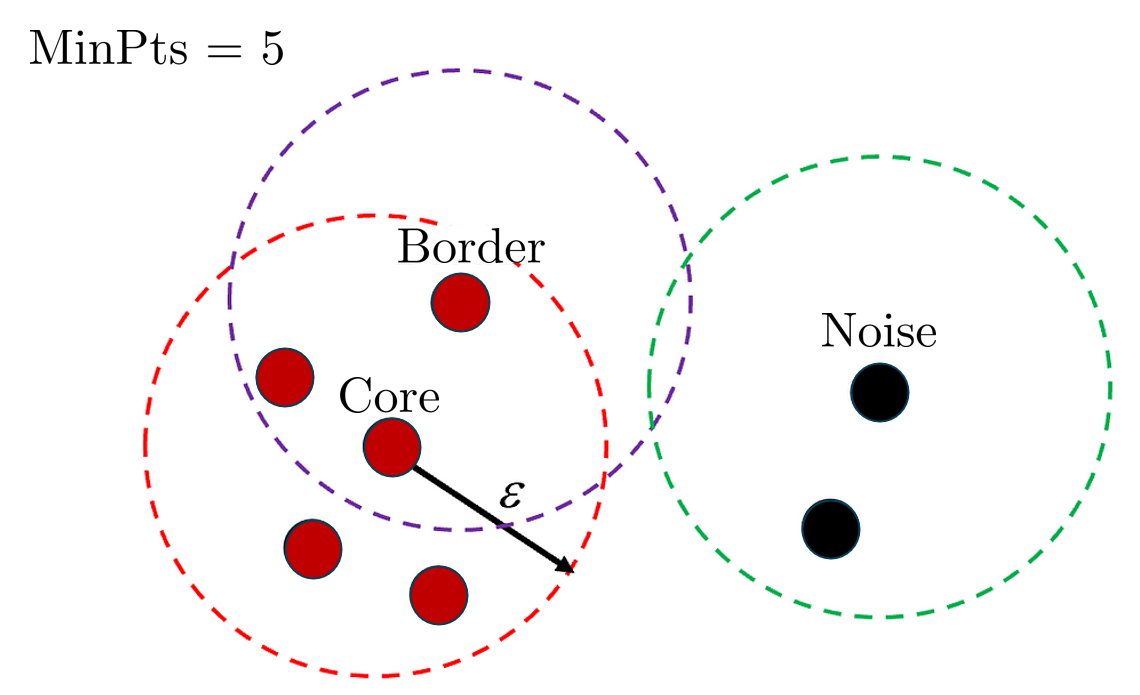
\includegraphics[width=0.5\textwidth]{../figures/dbscan_diagram.png}
    \caption{DBSCAN illustration: in this diagram, minPts = 5. 
    The red points form a cluster, with 4 core points because the area surrounding these points in an $\epsilon$ radius contain at least 5 points (including the point itself). A border point is also included in the red cluster because it is reachable from a core point. The black points are noise as they are neither core points nor directly-reachable.}
    \label{fig:dbscan}
\end{figure}

% An illustration of the DBSCAN algorithm is shown in Fig.\ref{fig:dbscan}. DBSCAN is particularly effective in identifying islands in 2D projections like UMAP because it clusters based on local density, allowing for the detection of irregularly shaped clusters without requiring predefined cluster numbers. 

% We also directly cluster the untouched embeddings that are of dimension $d = 128$, before we use dimensionality reduction techniques. To do so, we use k-Means \cite{udl} clustering from \verb|scikit-learn|. K-means is a centroid-based clustering algorithm that partitions a dataset into \( k \) clusters, where \( k \) is a user-specified parameter. The algorithm works by initialising \( k \) centroids, assigning each data point to the nearest centroid, and iteratively updating the centroids to minimise the variance within each cluster until convergence. We use the silhouette score \cite{silhouette} to evaluate the quality of the clustering, and we choose a reasonable value that balances the number of clusters and the quality of the clustering. We then project the embeddings to a 2D space using UMAP, and examine the spectra and images of the clusters formed.

An illustration of the DBSCAN algorithm is shown in Fig.\ref{fig:dbscan}. DBSCAN is particularly effective in identifying islands in 2D projections, such as those produced by UMAP, due to its density-based clustering approach. This method allows for the detection of irregularly shaped clusters without the need for predefined cluster numbers.

We also perform clustering on the original 128-dimensional embeddings before applying any dimensionality reduction techniques. For this purpose, we utilise the k-Means clustering  algorithm \cite{udl} from \verb|scikit-learn| . K-Means is a centroid-based clustering algorithm that partitions a dataset into \( k \) clusters, where \( k \) is a user-specified parameter. The algorithm operates by initialising \( k \) centroids, assigning each data point to the nearest centroid, and iteratively updating the centroids to minimise within-cluster variance until convergence. We evaluate the clustering quality using the silhouette score \cite{silhouette} to choose an appropriate \( k \) that balances the number of clusters and clustering quality. Subsequently, we project the embeddings to a 2D space using UMAP and examine the spectra and images of the clusters formed.





%--------------------------------------

\section{Results}
\label{sec:results}
In this section, we present the results of our AstroCLIP reproduction and extension. Where appropriate, we compare our results to the original work (v1) \cite{astroclip} and discuss possible reasons for any discrepancies. A discussion on the implications of our results and potential future work is also provided.

\subsection{Loss Curves}

Fig.\ref{fig:loss} shows the average InfoNCE loss per epoch for the training and validation sets during the cross-modal contrastive training. It is important to note that validation loss in the context of the contrastive framework is not a direct measure of performance but rather a proxy for the model's generalisation ability, as the training does not involve any labelled data.

\begin{figure}[H]
    \centering
    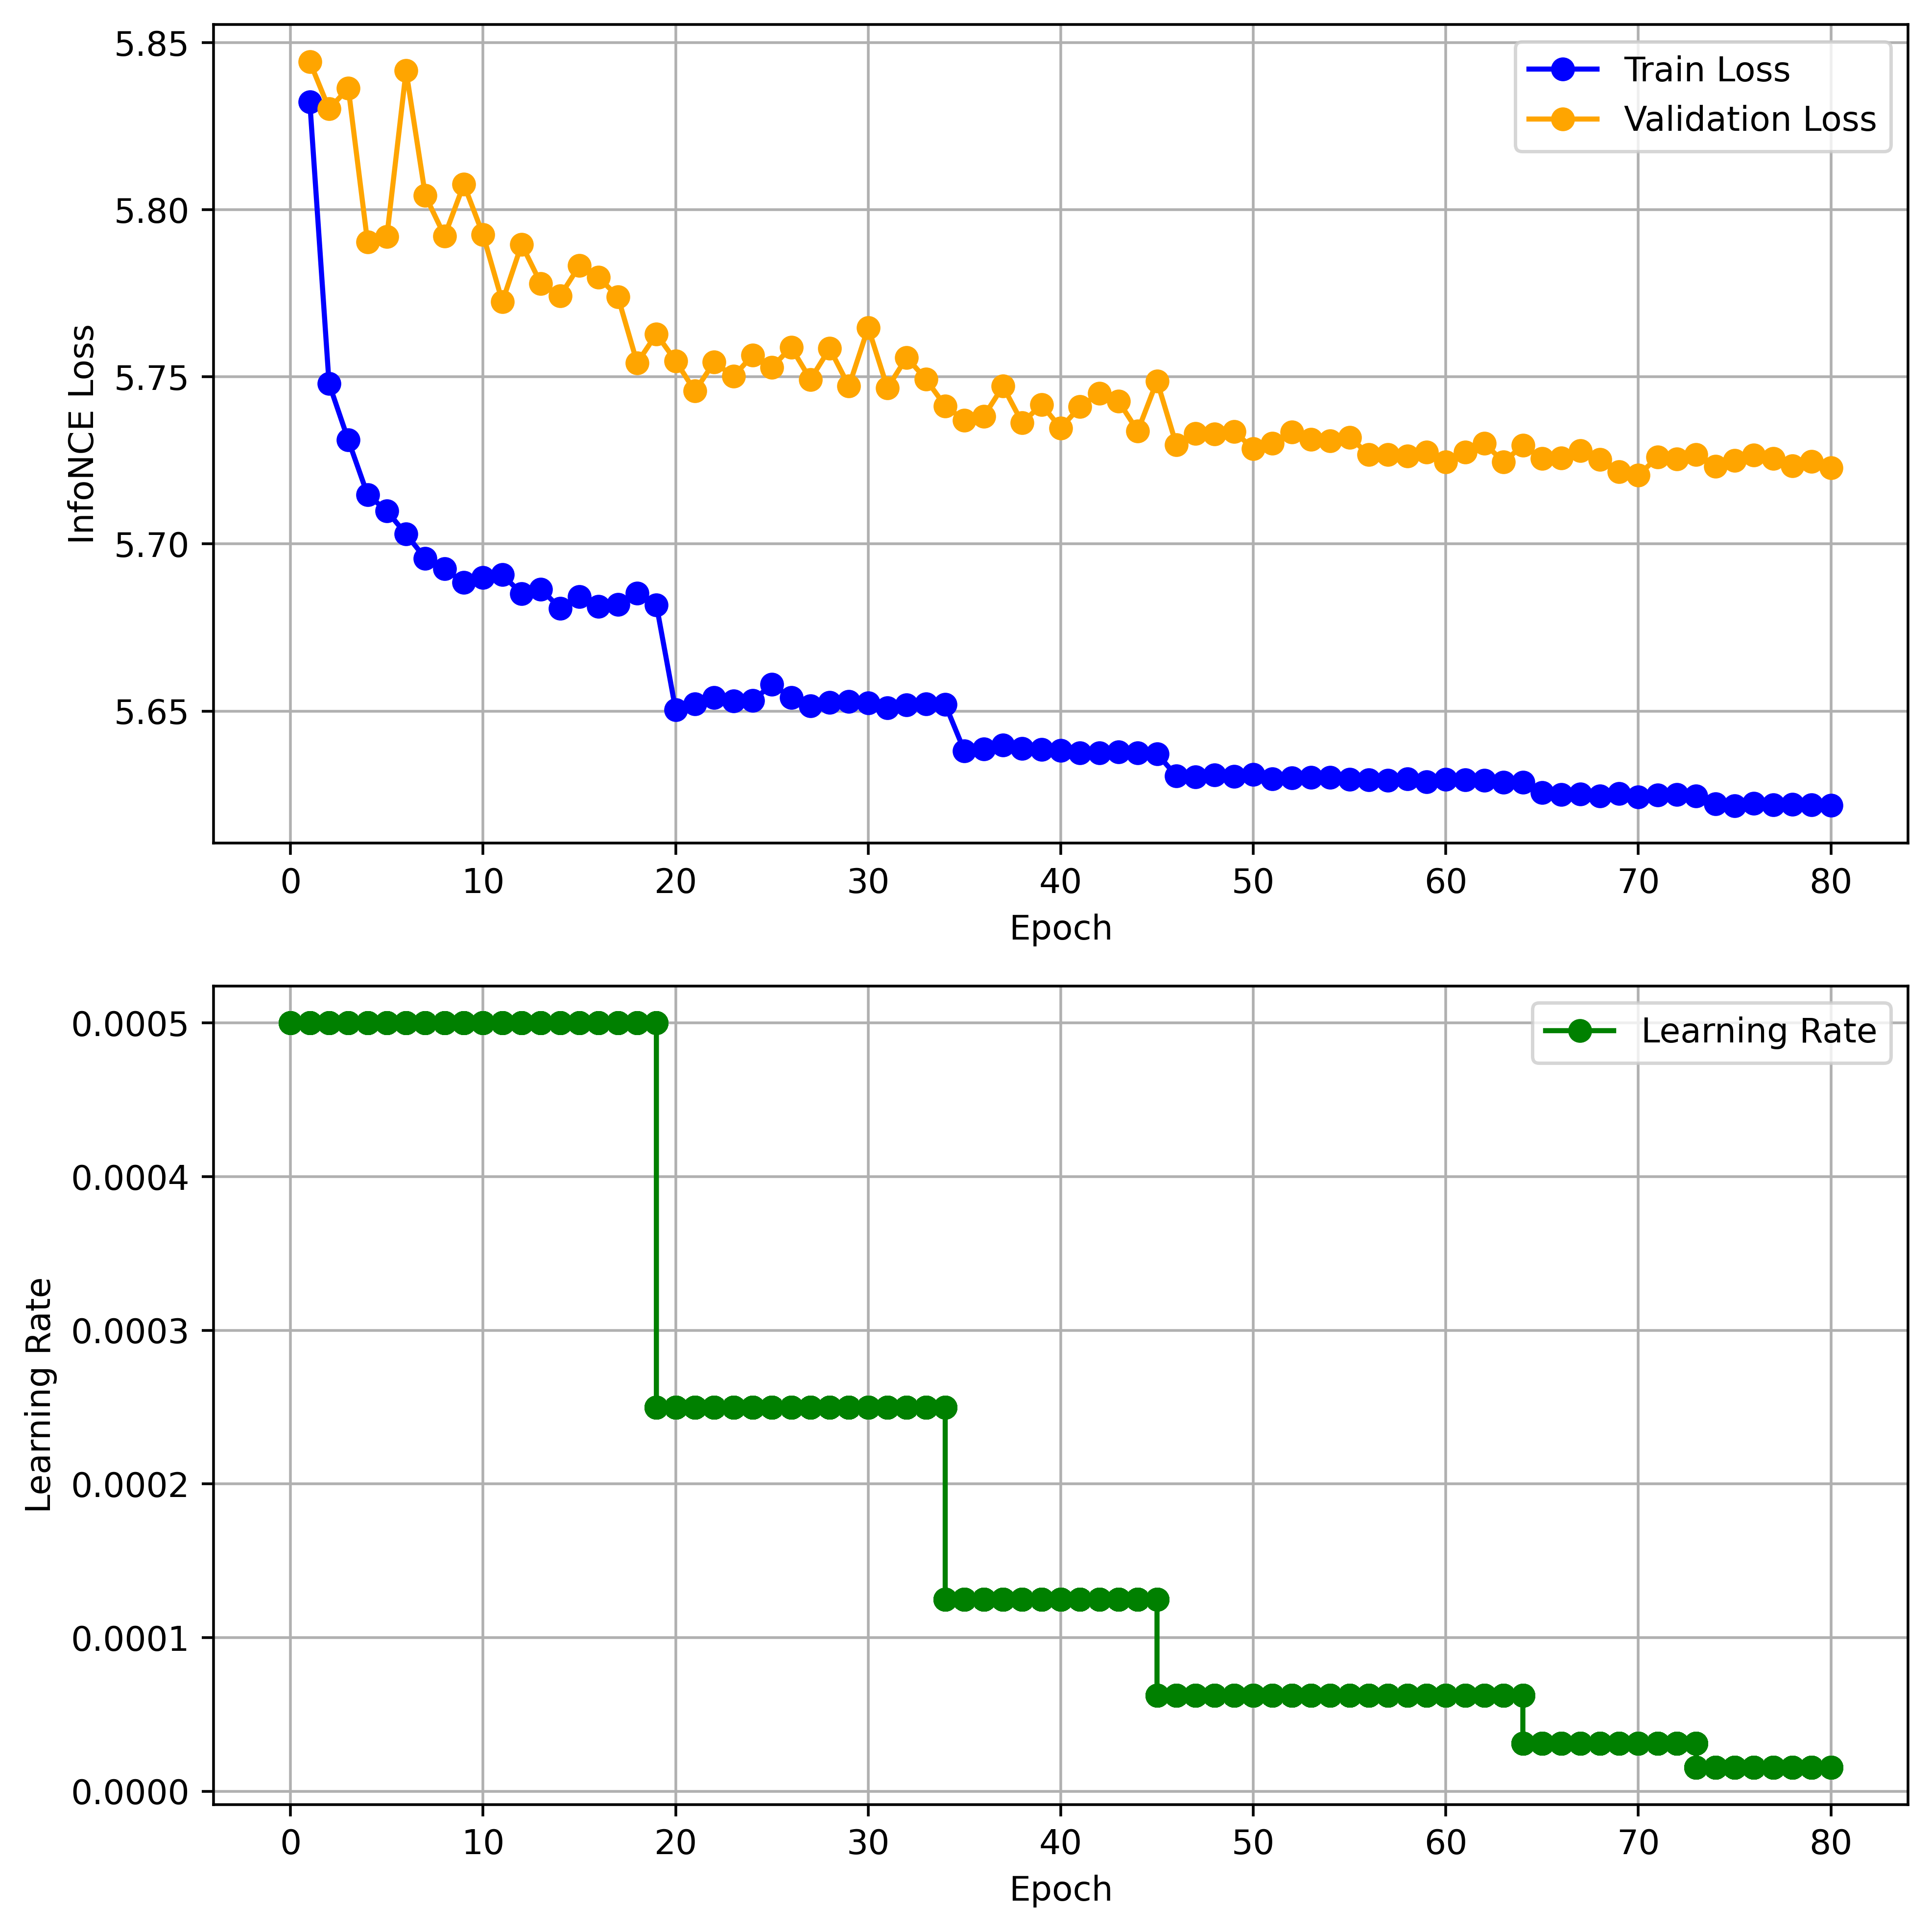
\includegraphics[width=0.8\textwidth]{../figures/training_plot.png}
    \caption{Average InfoNCE loss per epoch for training and validation sets during constrastive training (top), and the learning rate schedule (bottom). The learning rate is reduced by a factor of 2 if the validation loss does not improve for 5 epochs.}
    \label{fig:loss}
\end{figure}

Both the training and validation losses decrease steadily over the 80 epochs, indicating that the model is effectively learning to align the image and spectrum embeddings in the shared latent space. The validation loss is consistently higher than the training loss, as expected, but it does not diverge significantly nor begin to increase, suggesting that the model is not overfitting. Whenever the training loss plateaus for five epochs, the learning rate is reduced by a factor of two, resulting in a further decrease in the loss. This suggests that the model is prone to overshooting the optimal parameters and that the learning rate schedule is effective in mitigating this. The loss continues to decrease, albeit at a slower rate, until the end of the training. This could imply that the model has not fully converged and might benefit from additional training. The original work does not provide loss curves, learning rates, or the number of epochs, and thus a direct comparison is not possible.









\subsection{Query Retrieval}
Fig.\ref{fig:retrieval} showcases the three most similar galaxies (based on the cosine similarity of their embeddings) to four random query galaxy for all possible combinations of modalities. By construction, for in-modal searches the best match for the query galaxy is the galaxy itself, as the similarity score is 1.0. The model is able to retrieve galaxies that are visually similar to the query galaxy. The colour is well preserved in both in-modal and cross-modal searches, indicating that the model has learned to align the image and spectrum embeddings in the shared latent space. If the model was trained as a single-modal model, we would expect in-modal image searches to perform better than cross-modal searches. However, the model is able to retrieve visually similar galaxies in both cases, indicating that the structuring is informed by both modalities.  This is the reason why spectrum query - spectrum retrievals $S_C(\mathbf{z}^{\text{sp}}_q, \mathbf{z}^{\text{sp}}_j)$ are have similar images as well. 

\begin{figure}[H]
    \centering
    \begin{subfigure}{0.08\textwidth}
        \centering
        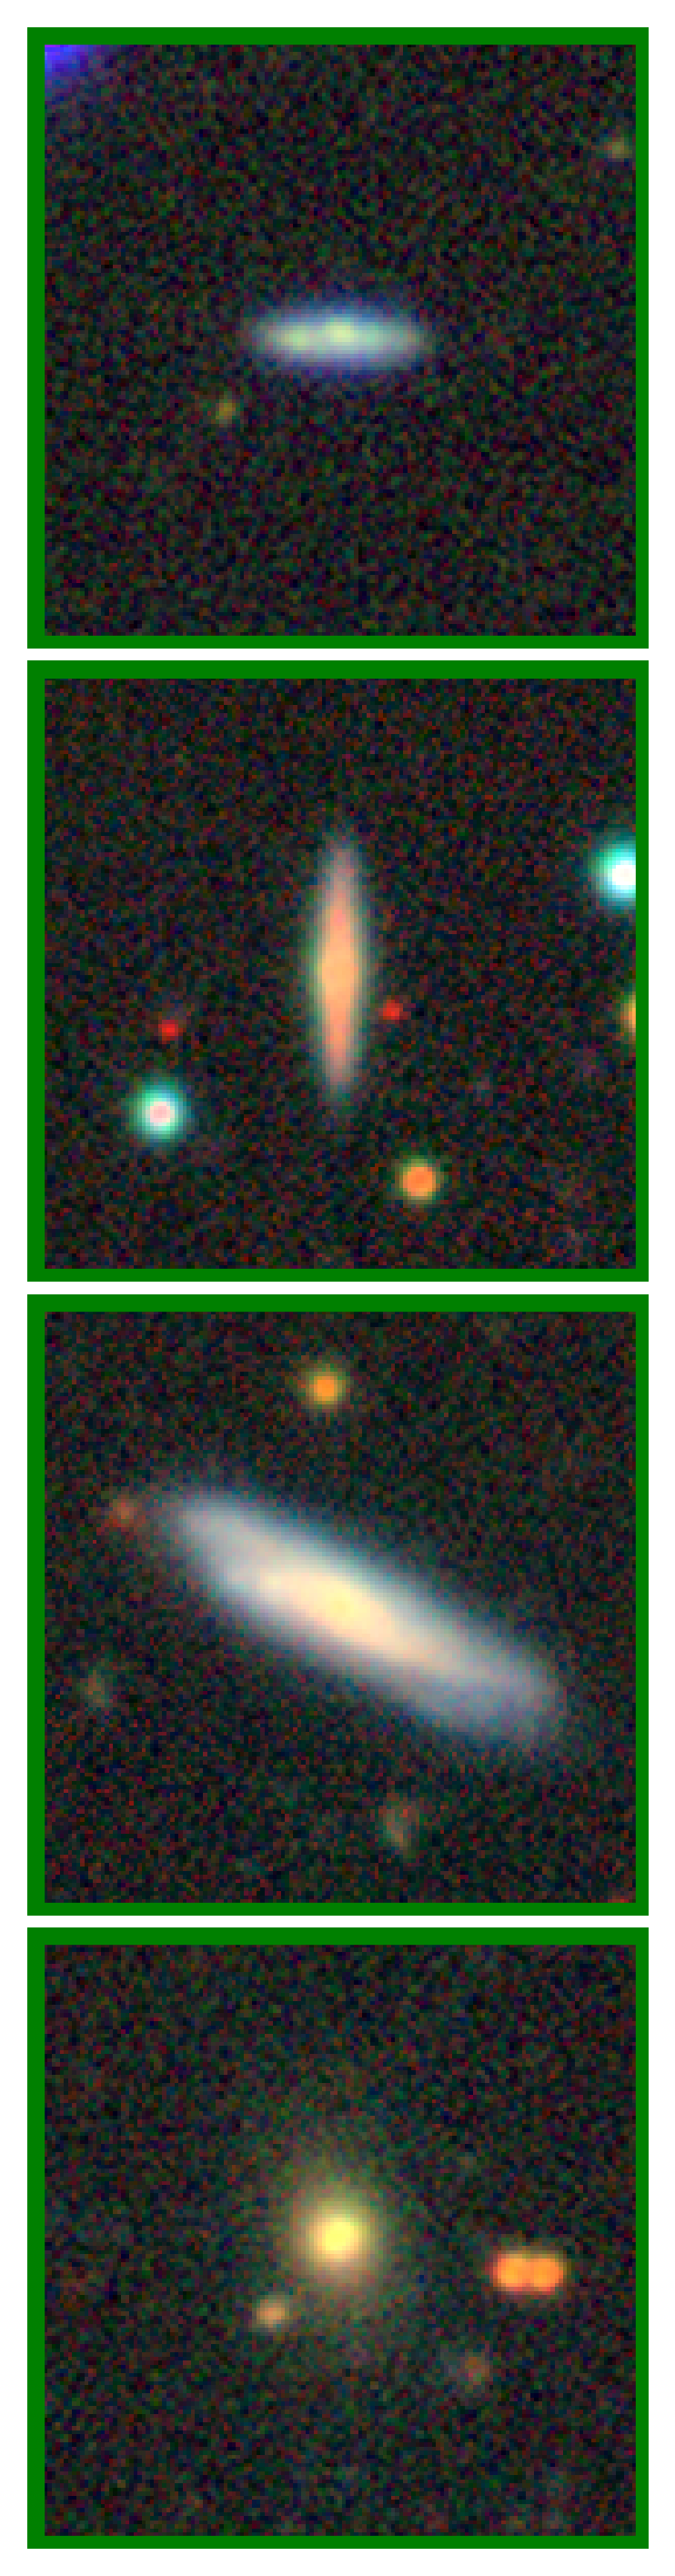
\includegraphics[height=0.21\textheight]{../figures/query_images.png}
        \caption{$\mathbf{z}_q$}
        \label{fig:retrieval_1}
    \end{subfigure}%
    \hfill
    \begin{subfigure}{0.22\textwidth}
        \centering
        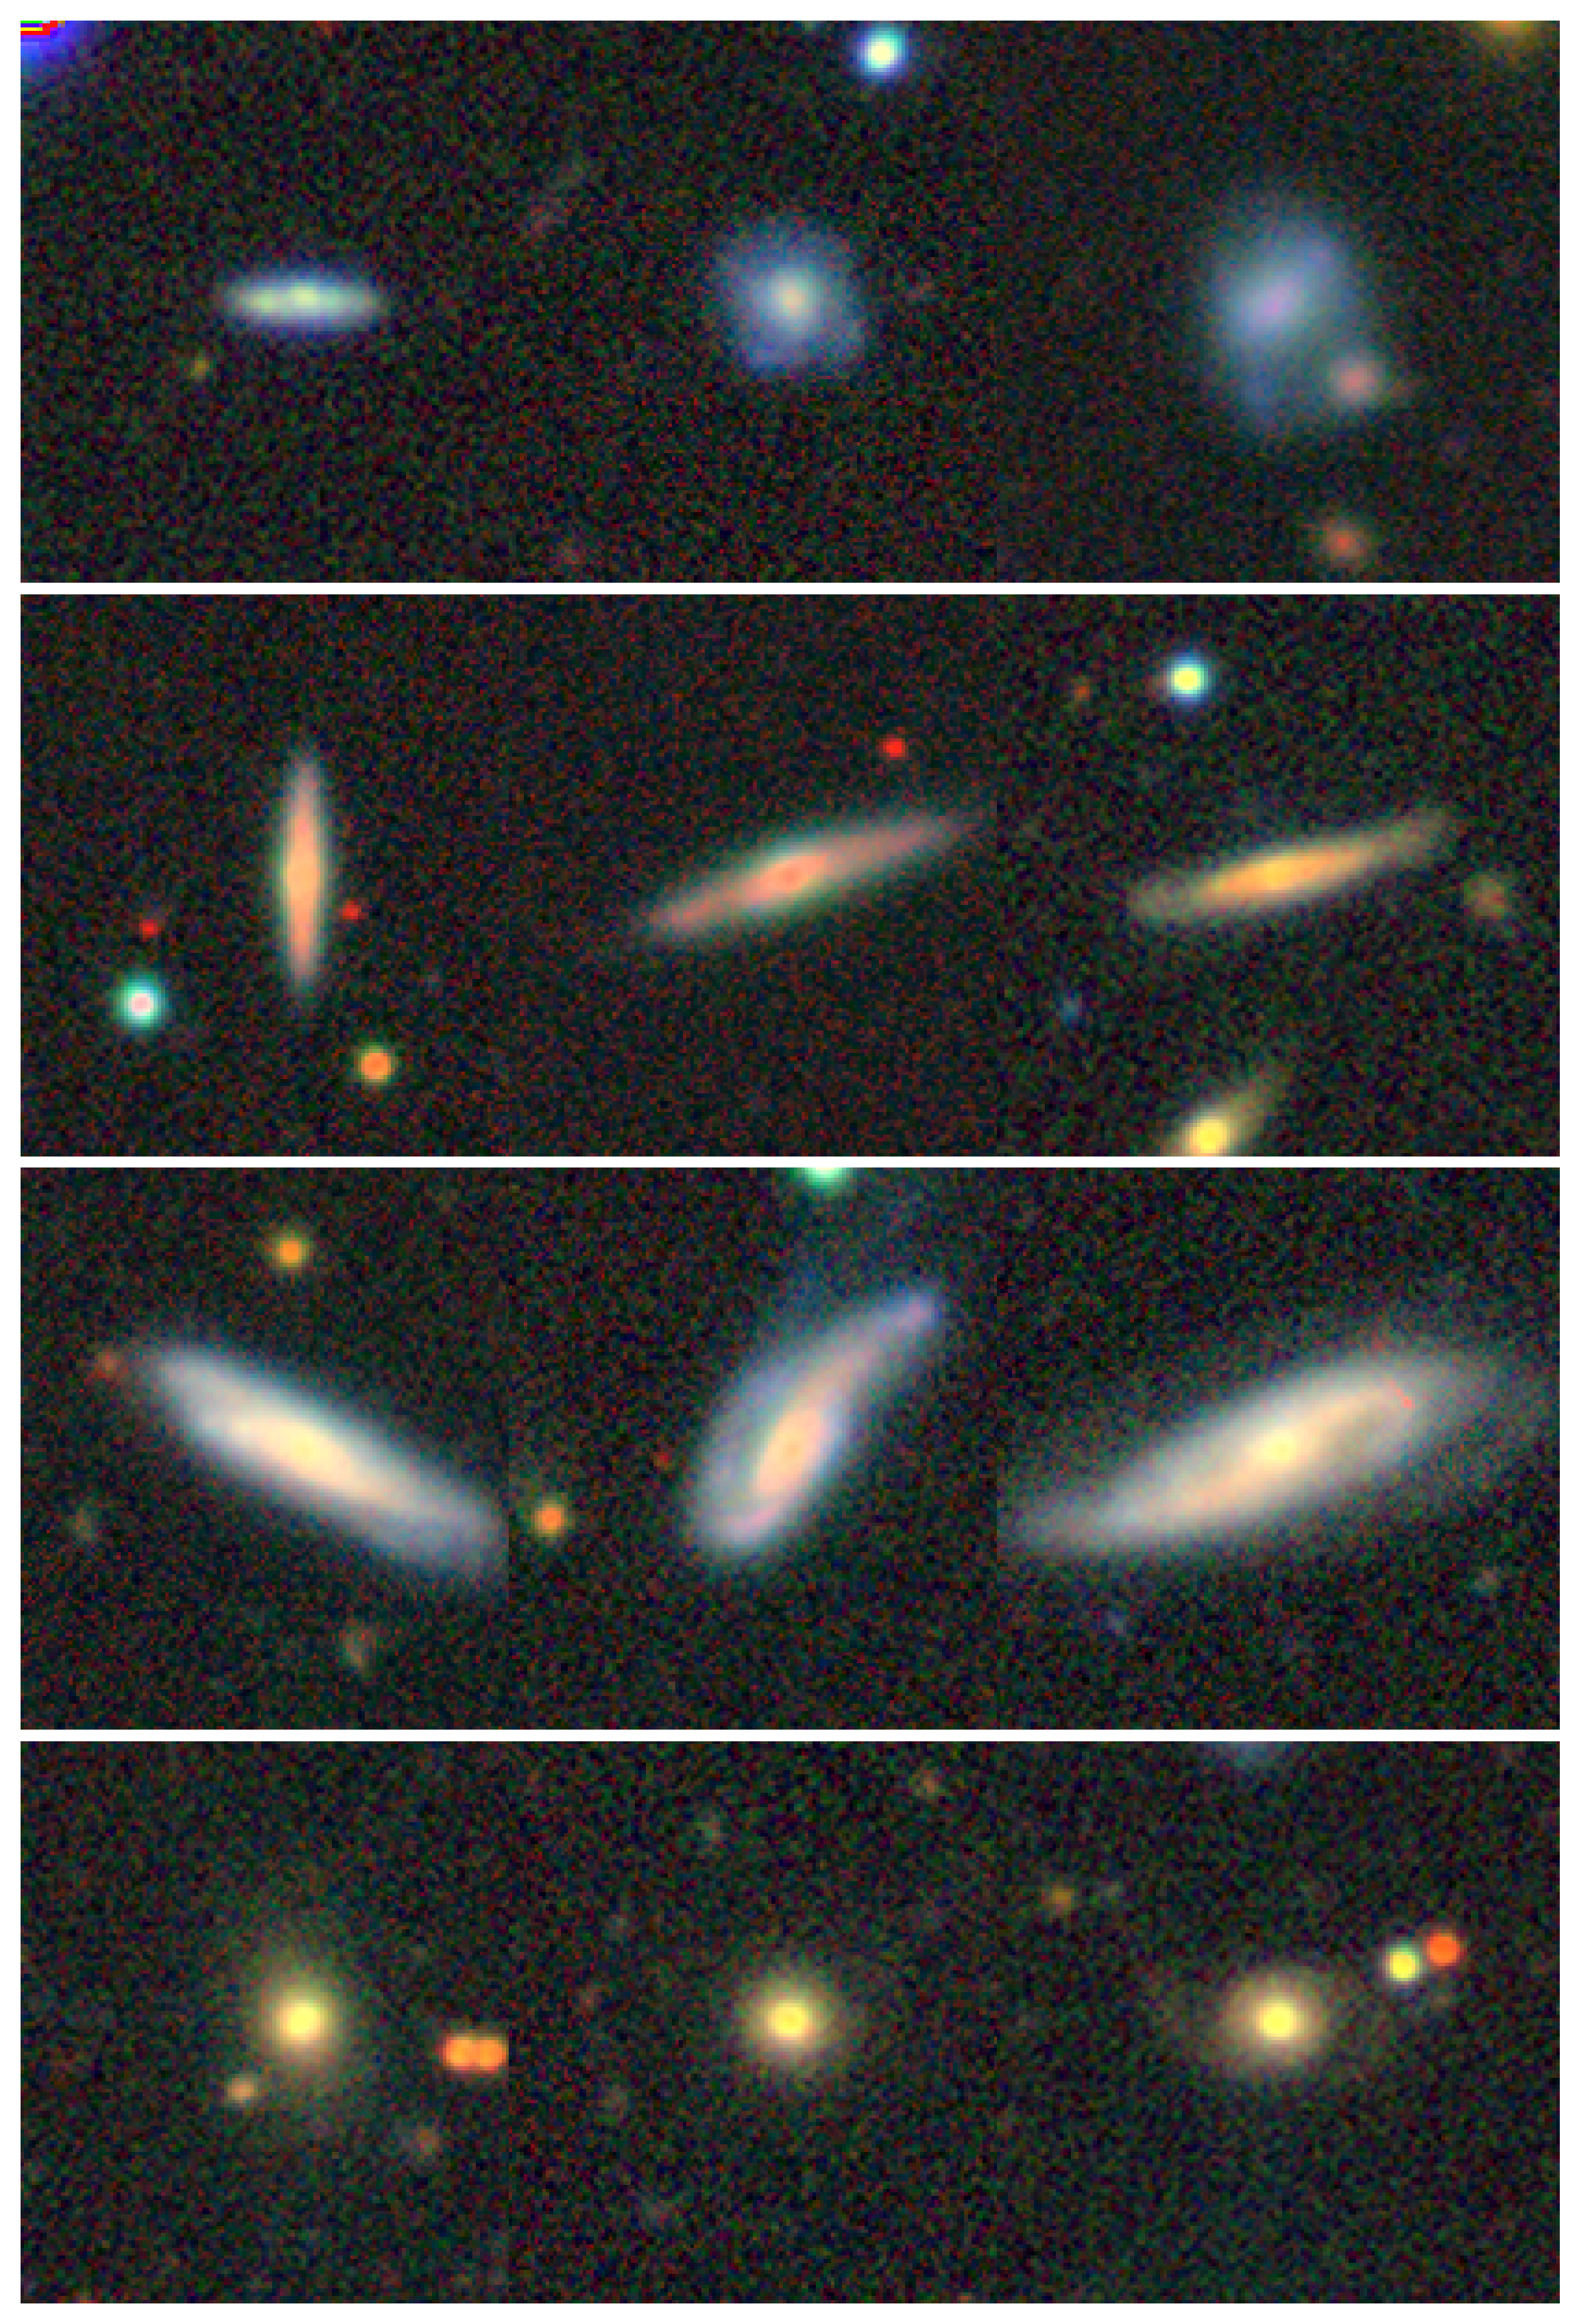
\includegraphics[height=0.21\textheight]{../figures/images_im_im.png}
        \caption{$S_C(\mathbf{z}_q^{\text{im}}, \mathbf{z}_j^{\text{im}})$}
        \label{fig:retrieval_2}
    \end{subfigure}%
    \hfill
    \begin{subfigure}{0.22\textwidth}
        \centering
        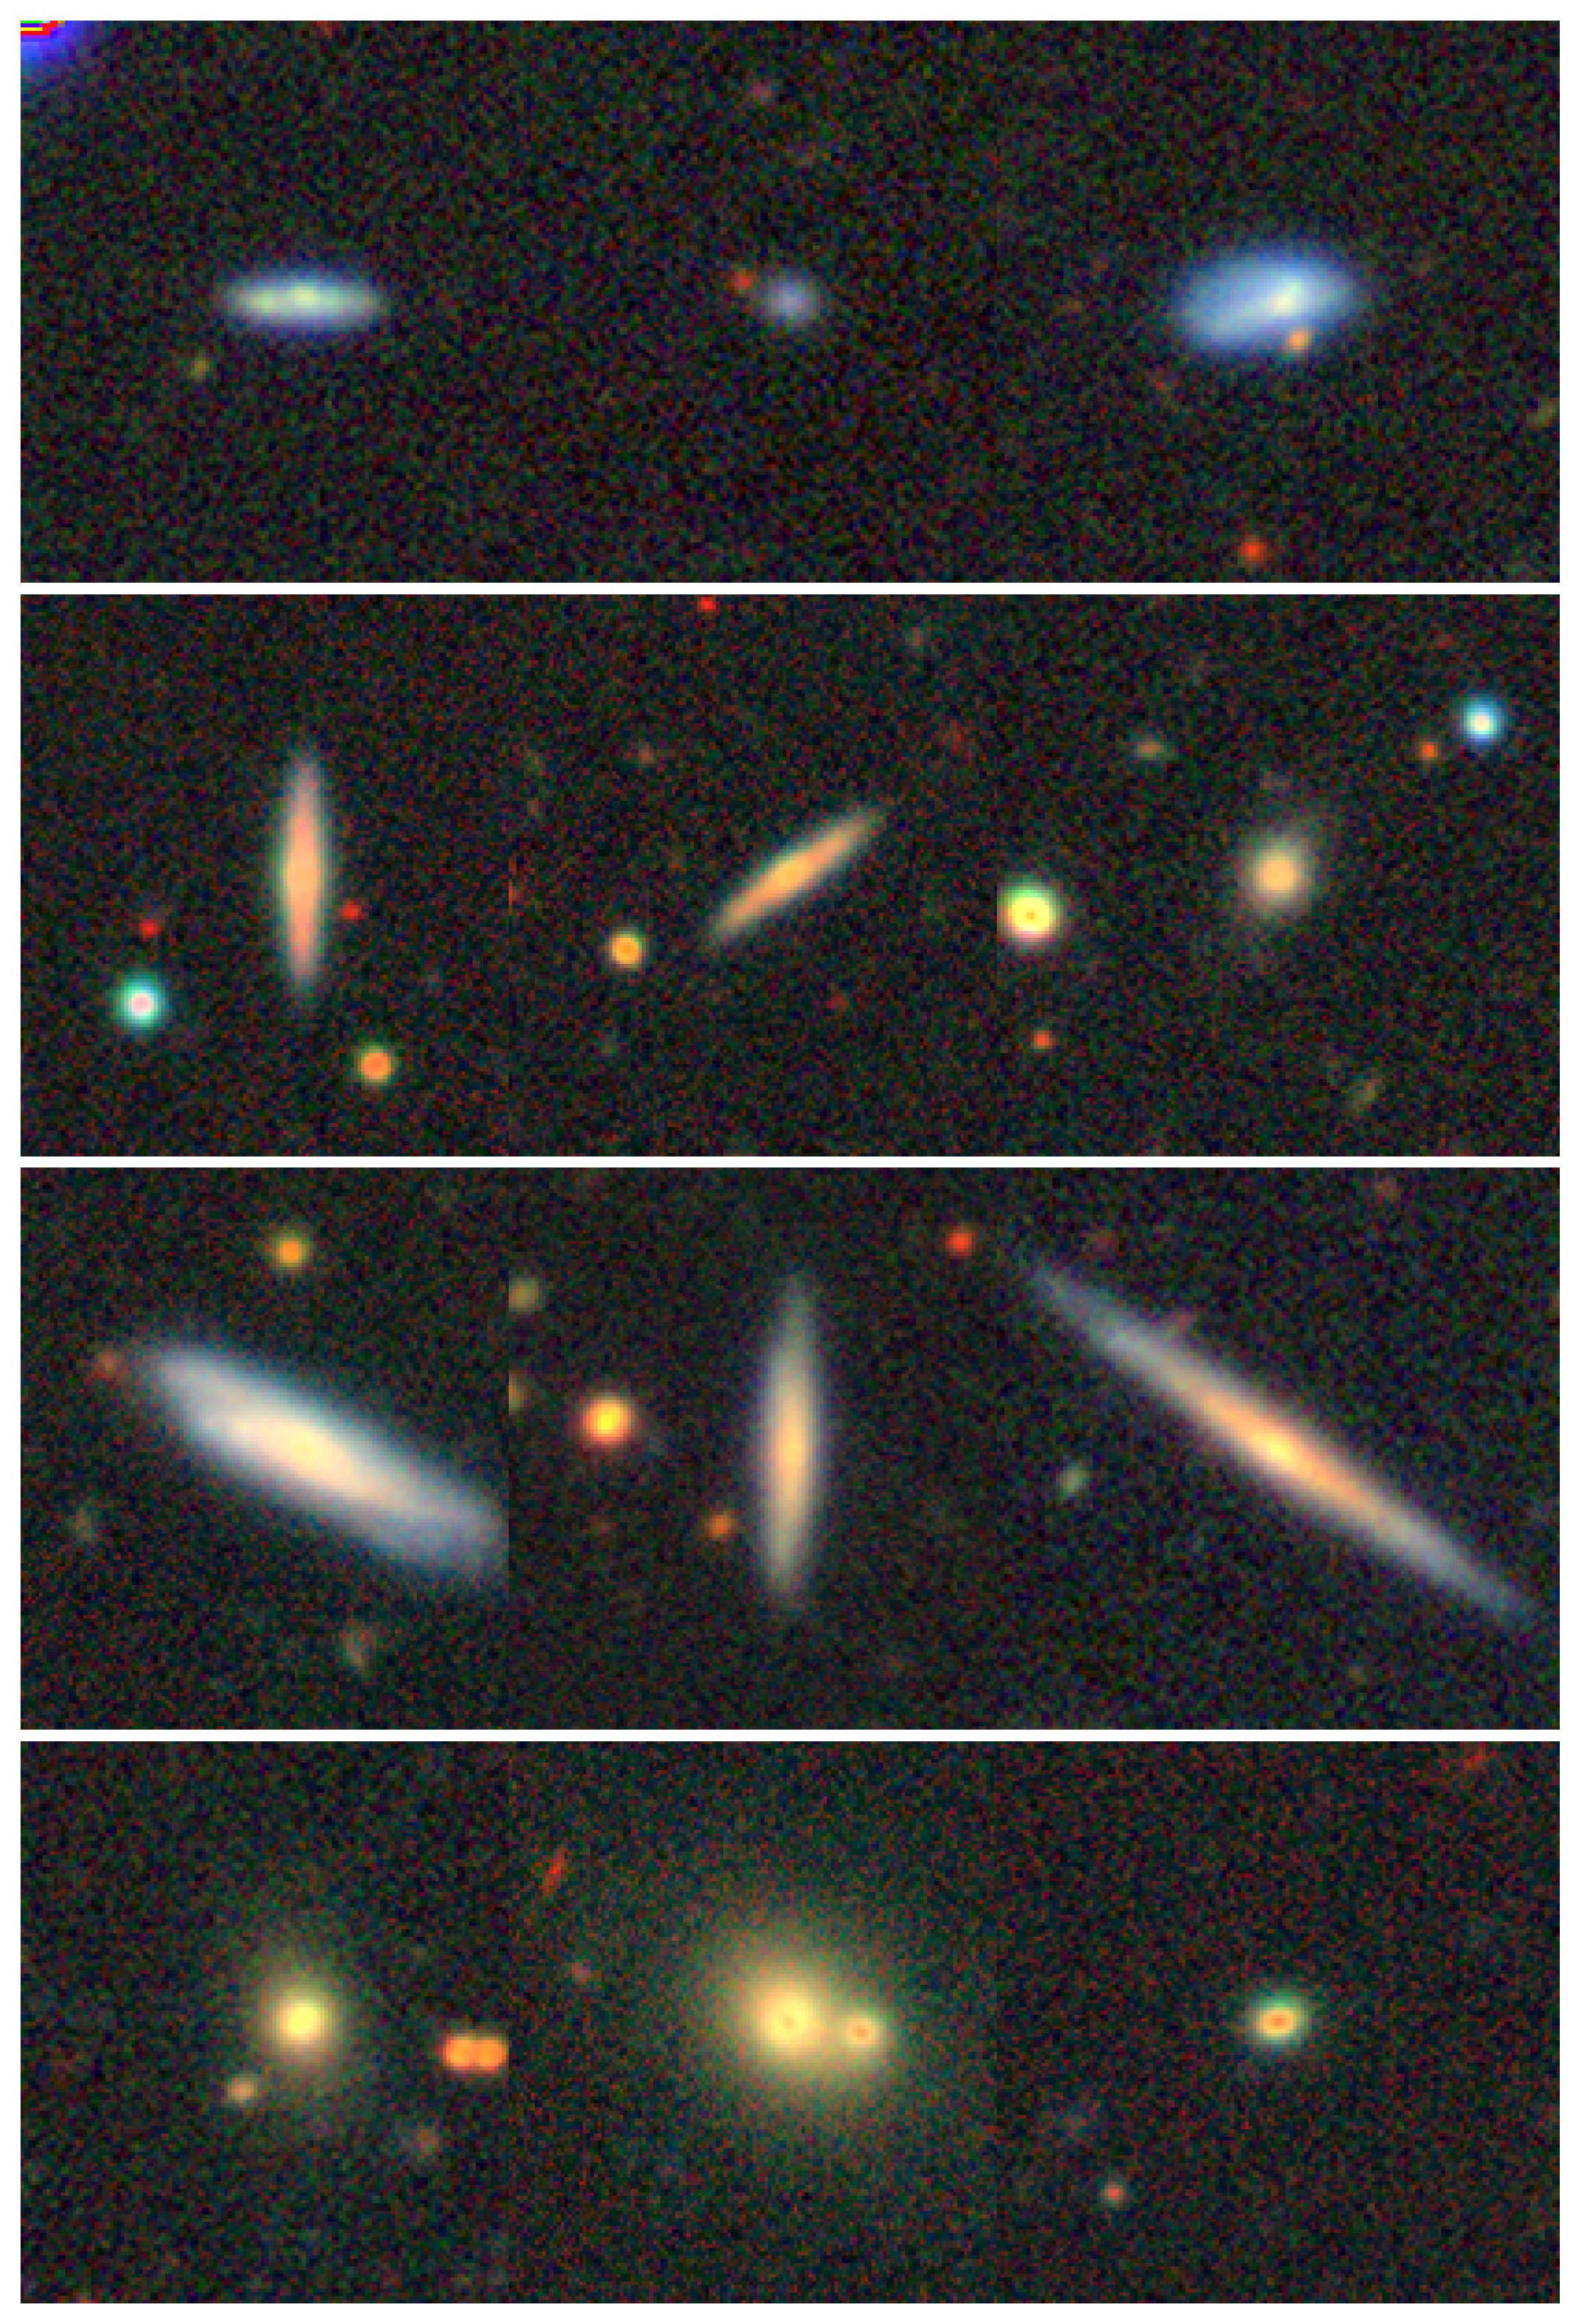
\includegraphics[height=0.21\textheight]{../figures/images_sp_sp.png}
        \caption{$S_C(\mathbf{z}_q^{\text{sp}}, \mathbf{z}_j^{\text{sp}})$}
        \label{fig:retrieval_3}
    \end{subfigure}%
    \hfill
    \begin{subfigure}{0.22\textwidth}
        \centering
        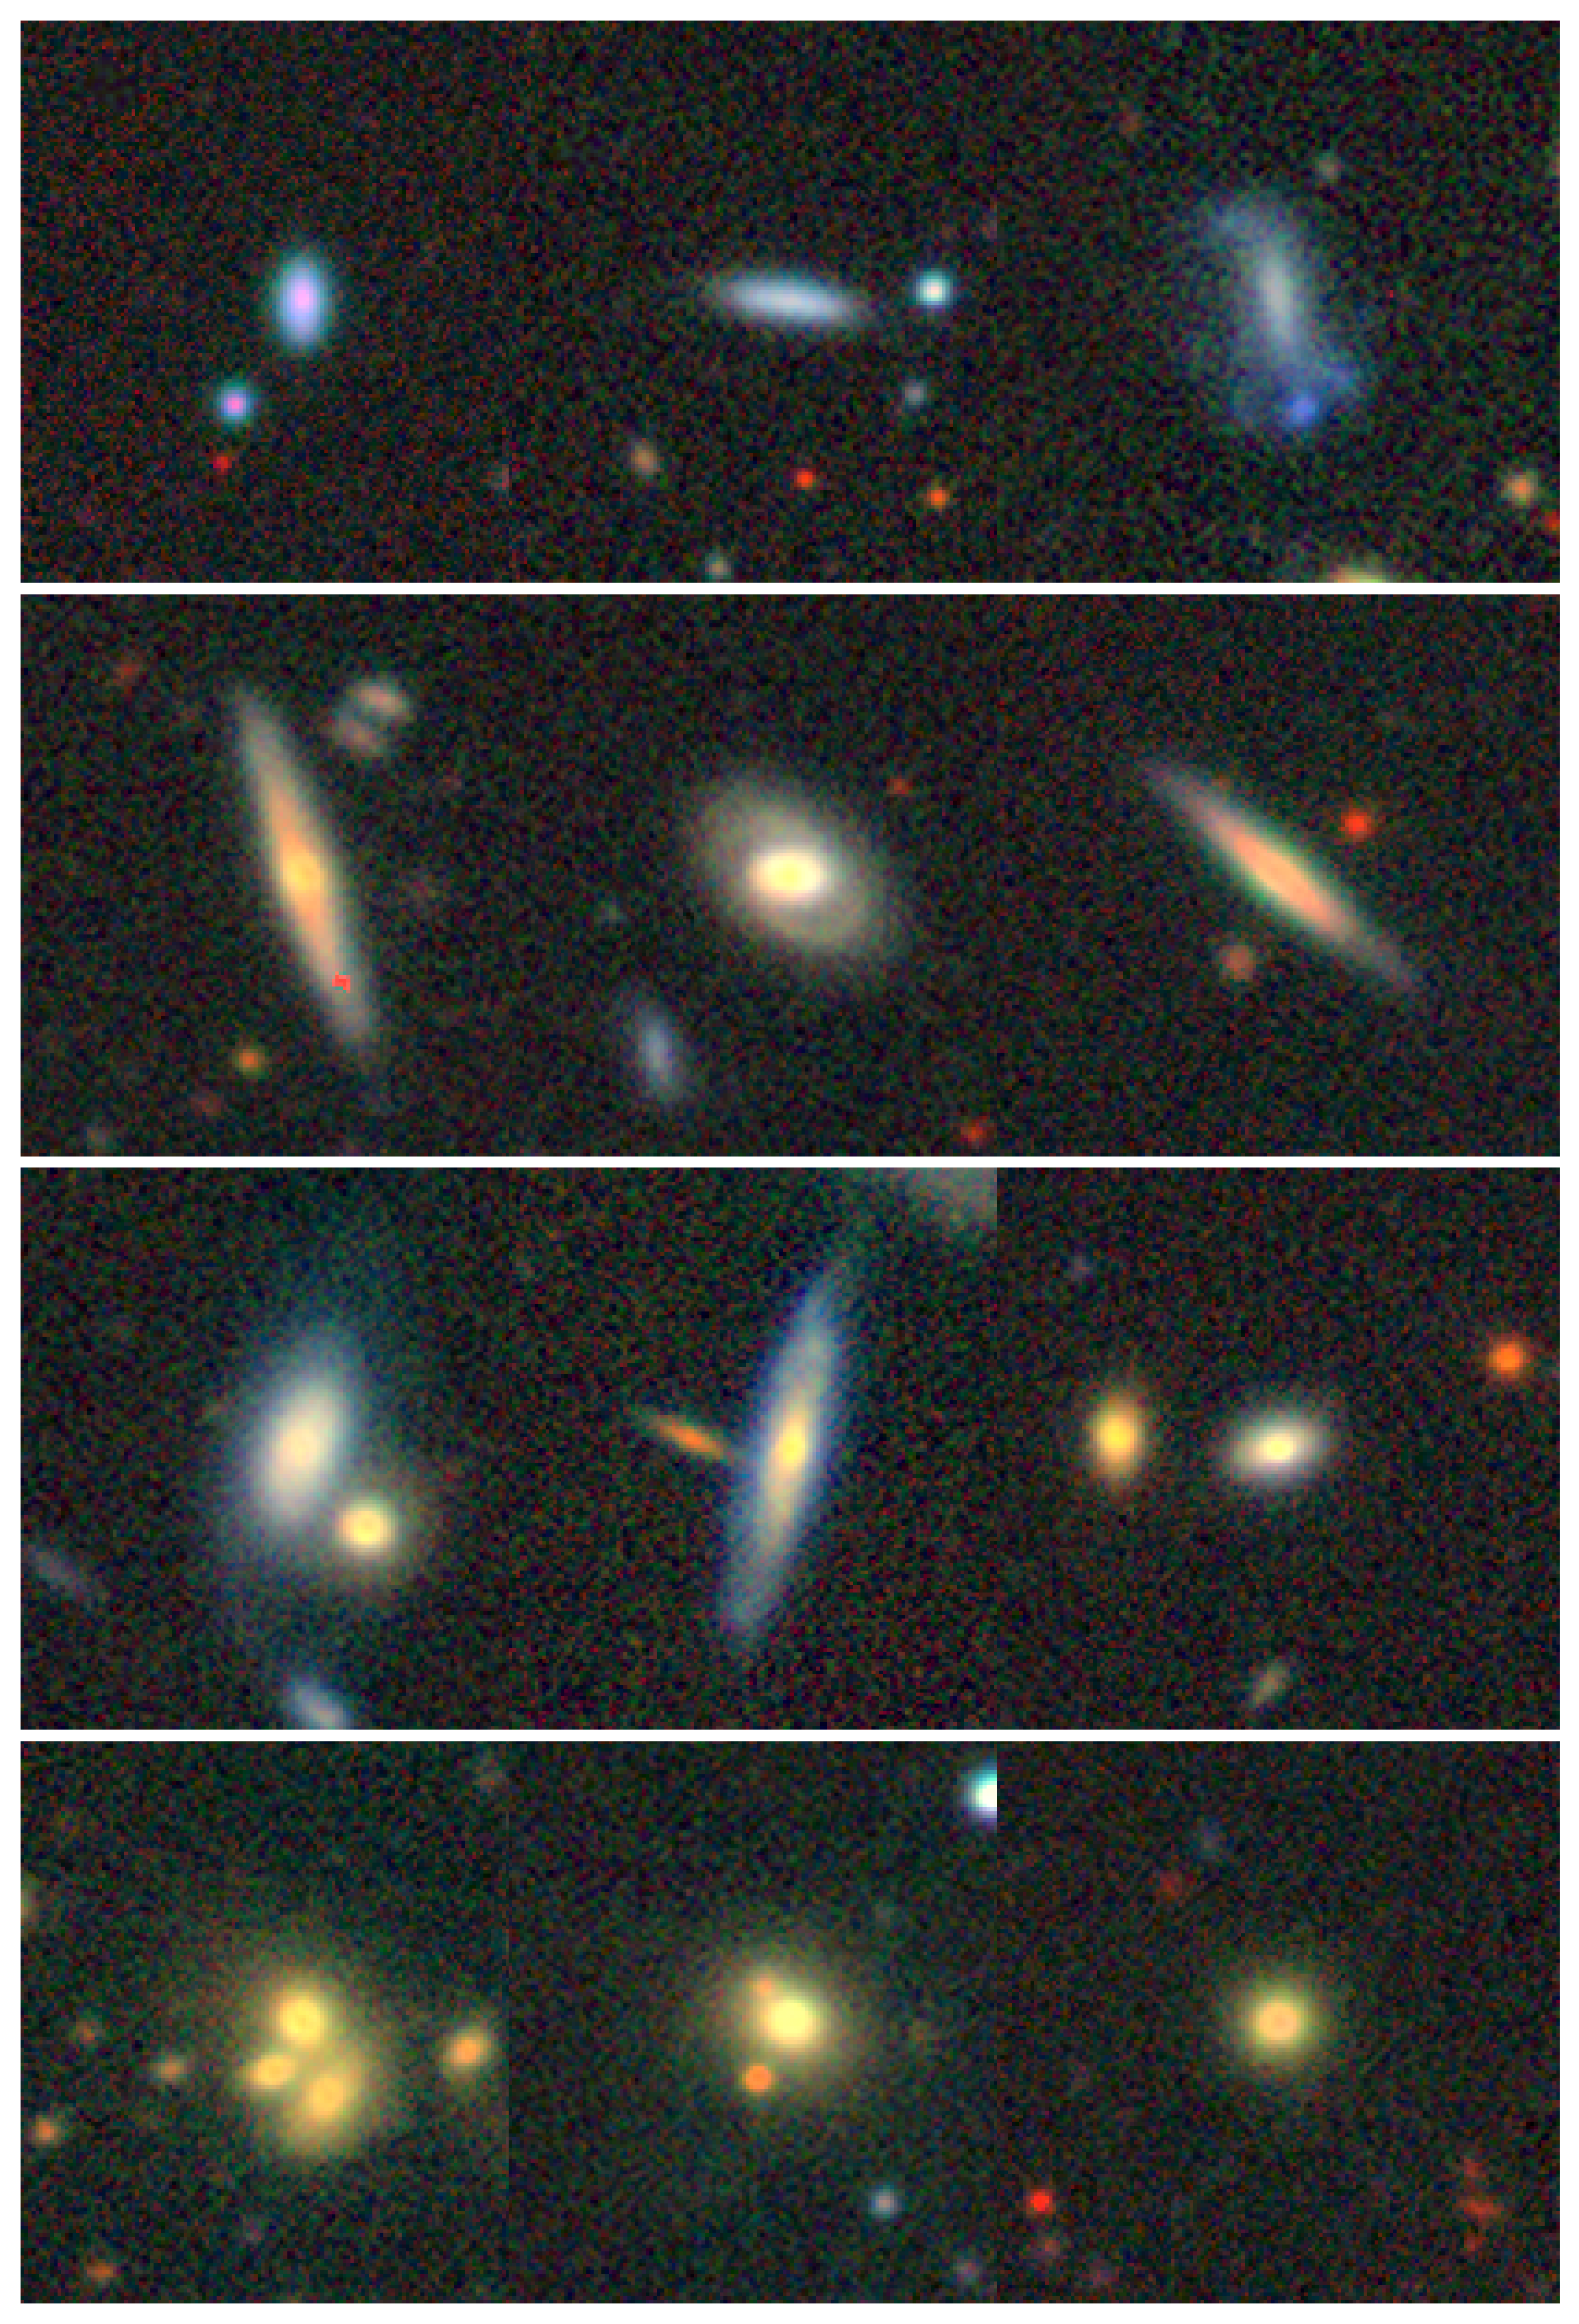
\includegraphics[height=0.21\textheight]{../figures/images_im_sp.png}
        \caption{$S_C(\mathbf{z}_q^{\text{sp}}, \mathbf{z}_j^{\text{im}})$}
        \label{fig:retrieval_4}
    \end{subfigure}%
    \hfill
    \begin{subfigure}{0.22\textwidth}
        \centering
        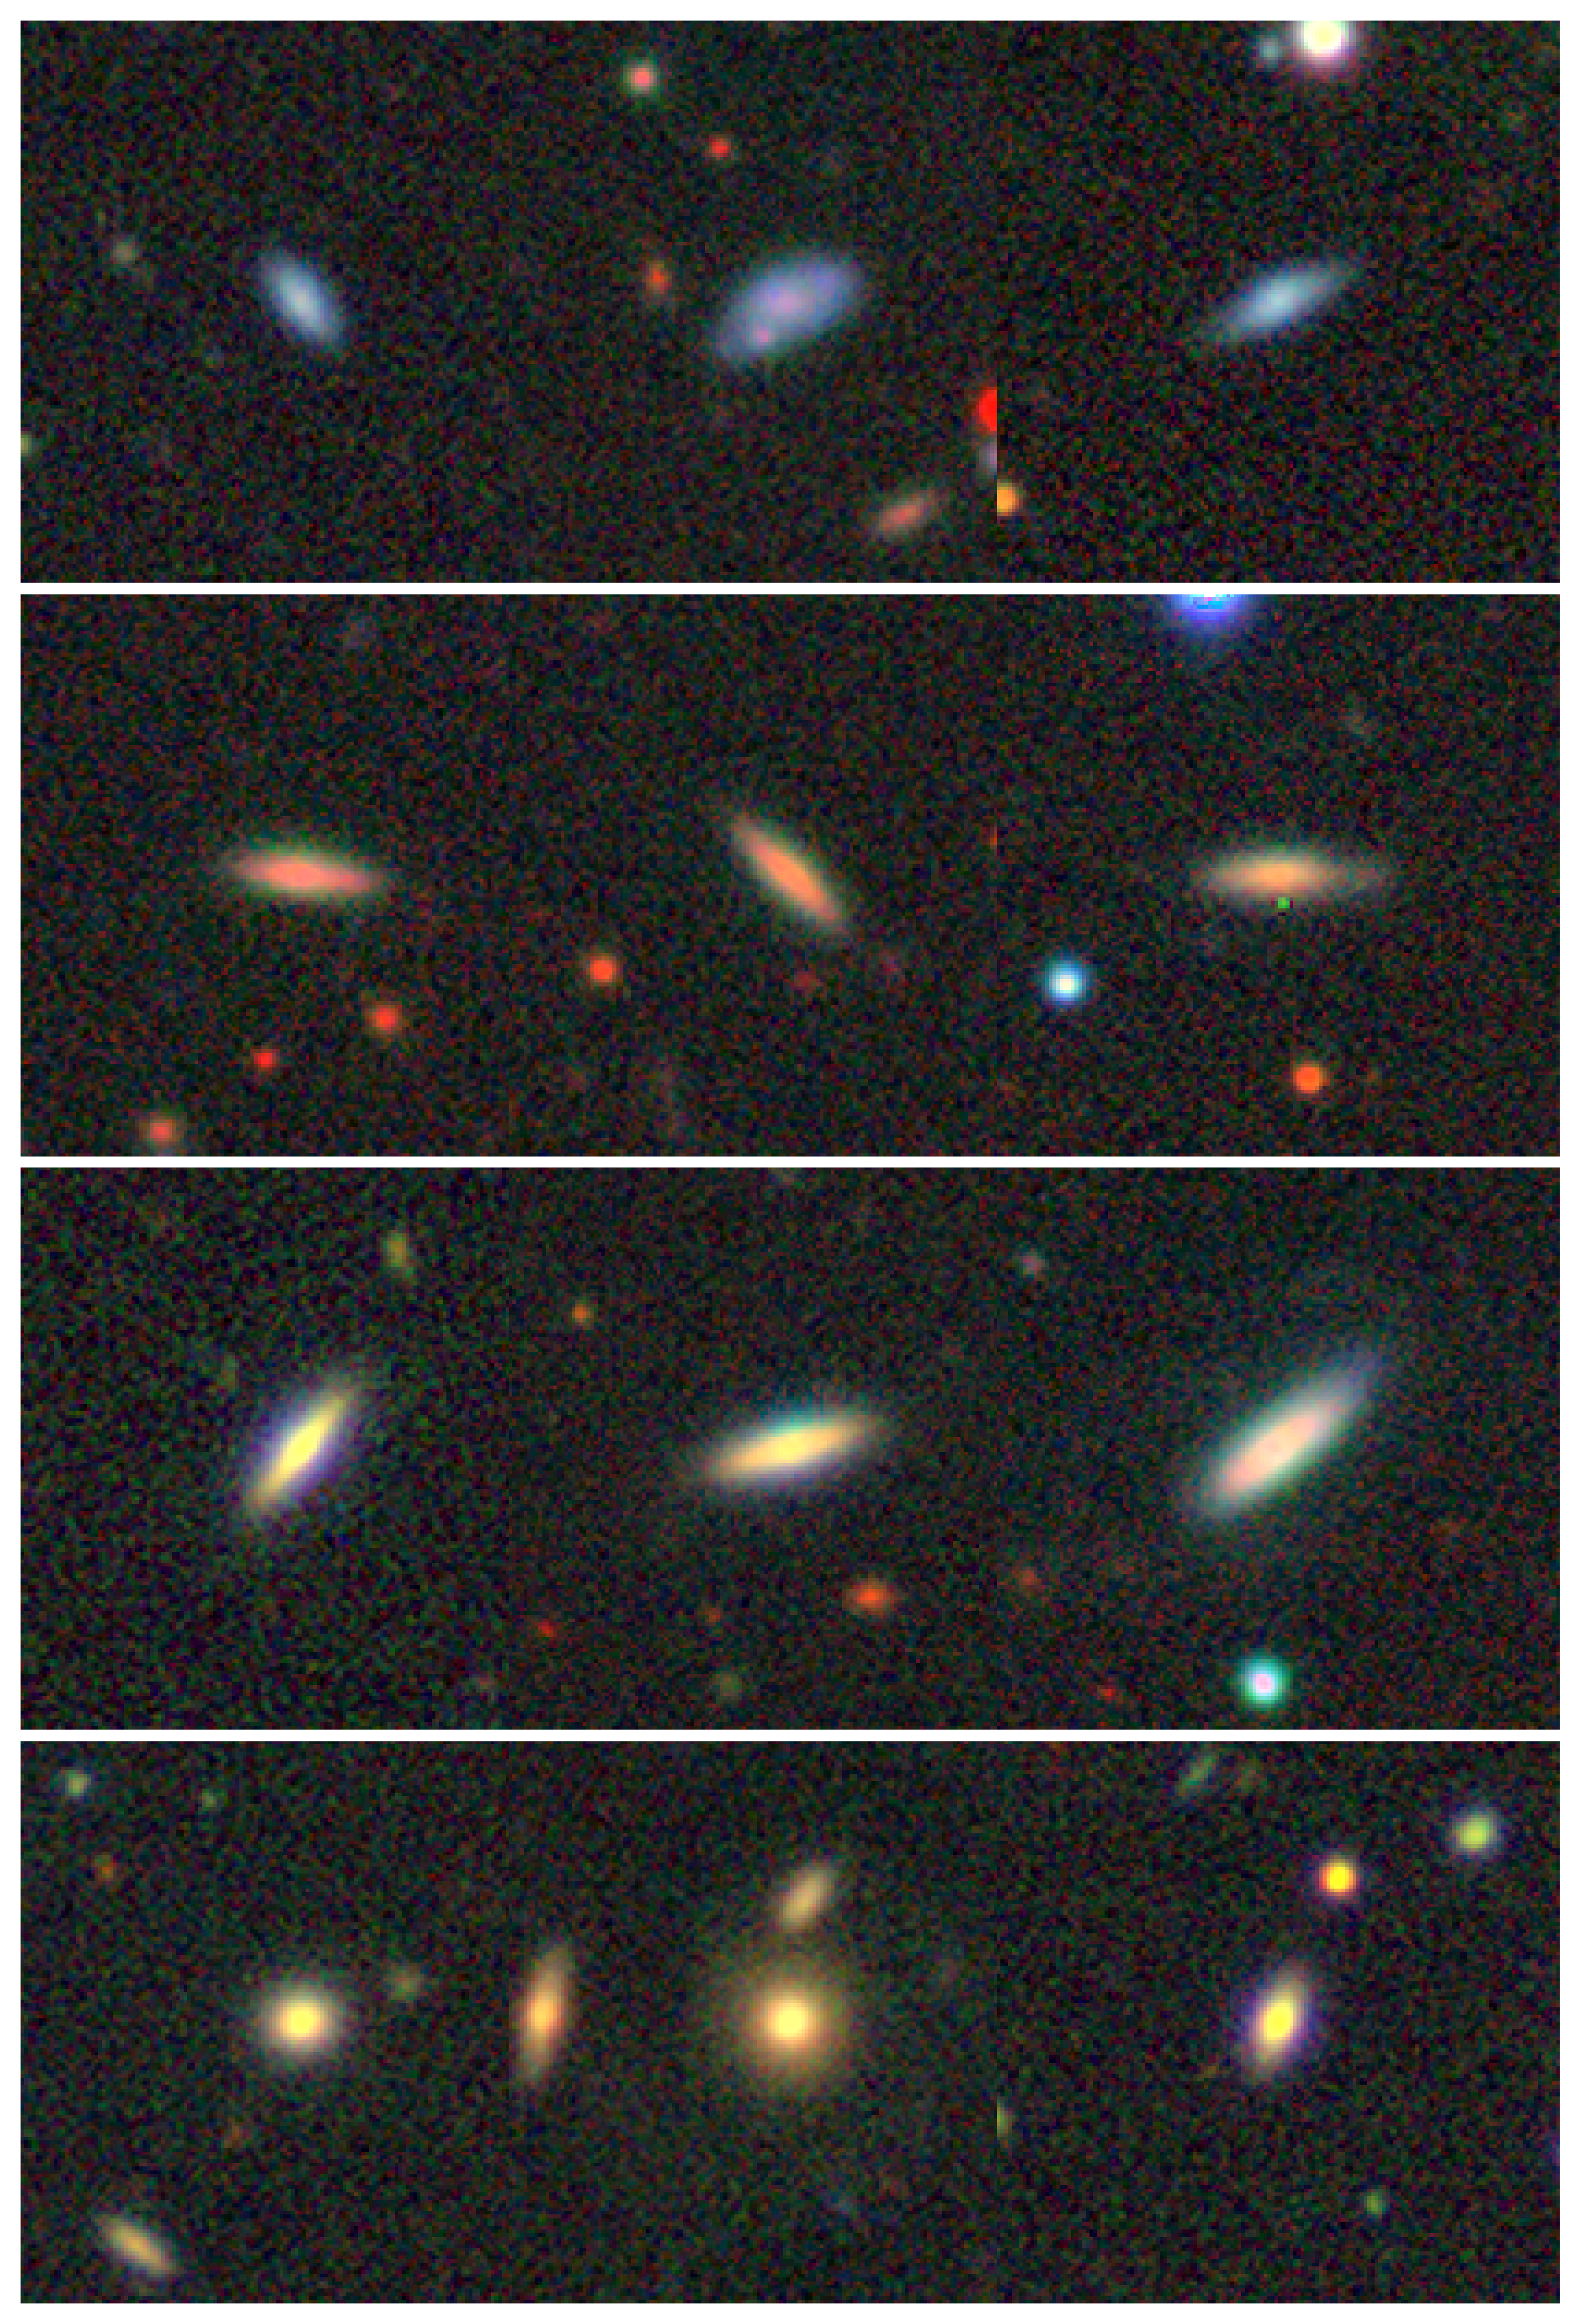
\includegraphics[height=0.21\textheight]{../figures/images_sp_im.png}
        \caption{$S_C(\mathbf{z}_q^{\text{im}}, \mathbf{z}_j^{\text{sp}})$}
        \label{fig:retrieval_5}
    \end{subfigure}
    \caption{Query retrieval for four galaxies in the validation set. The images in block (a) are the query galaxies. Block (b) shows the top 3 most similar galaxies to the query galaxy based on image-image embedding similarity. Block (c) shows the top 3 most similar galaxies to the query galaxy based on spectrum-spectrum embedding similarity. Blocks (d) and (e) show the top 3 most similar galaxies to the query galaxy based on spectrum-image and image-spectrum embedding similarity, respectively.}
    \label{fig:retrieval}
\end{figure}
We further illustrate the search capabilities of this model by presenting the retrieved spectra for some of query galaxies for all combinations of modalities in Fig.\ref{fig:spectral_retrieval}. The 5 most similar spectra are shown for each query galaxy. The model is largely able to retrieve spectra similar to the query galaxy, in all modality pair combinations. This is both in terms of the overall shape of the spectrum and the presence of specific spectral features, such as particular spikes. This further demonstrates the model's ability to align the image and spectrum embeddings in the shared latent space.


\begin{figure}[H]
    \centering
    % Add vertical space to extend into the top margin
    \vspace*{-1.3cm}

    % First row
    \begin{subfigure}[b]{0.45\textwidth}
        \centering
        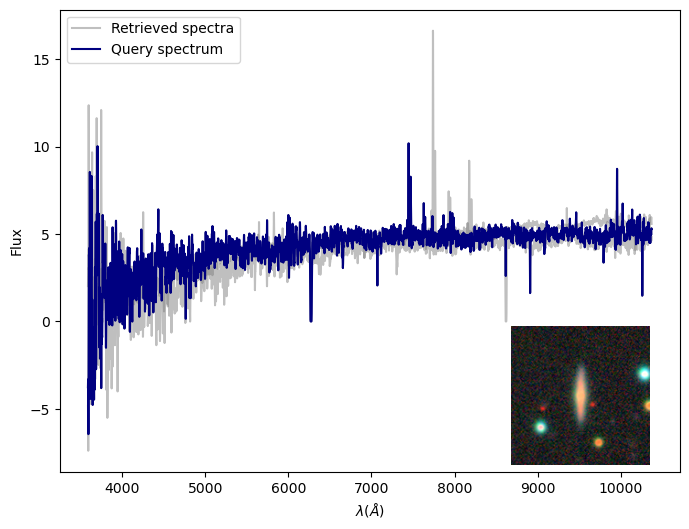
\includegraphics[width=\textwidth]{../figures/spectral_retrieval_im_im_1}
        \caption{$S_C(\mathbf{z}_q^{\text{im}}, \mathbf{z}_j^{\text{im}})$}
        \label{fig:im_im_1}
    \end{subfigure}%
    \hfill
    \begin{subfigure}[b]{0.45\textwidth}
        \centering
        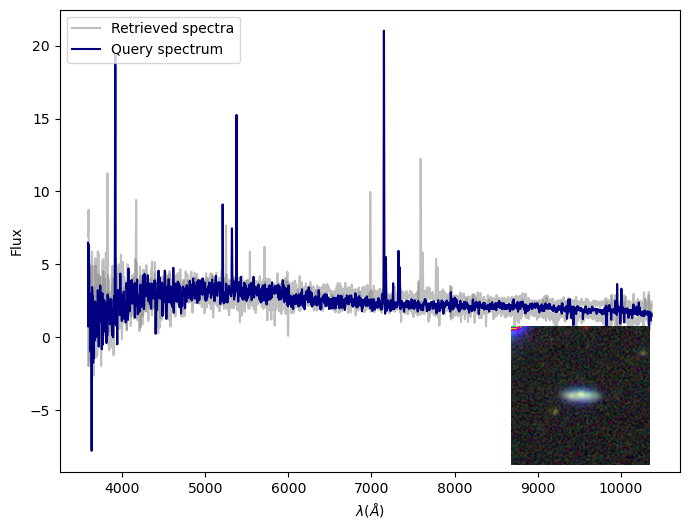
\includegraphics[width=\textwidth]{../figures/spectral_retrieval_im_im_2}
        \caption{$S_C(\mathbf{z}_q^{\text{im}}, \mathbf{z}_j^{\text{im}})$}
        \label{fig:im_im_2}
    \end{subfigure}

    % Second row
    \begin{subfigure}[b]{0.45\textwidth}
        \centering
        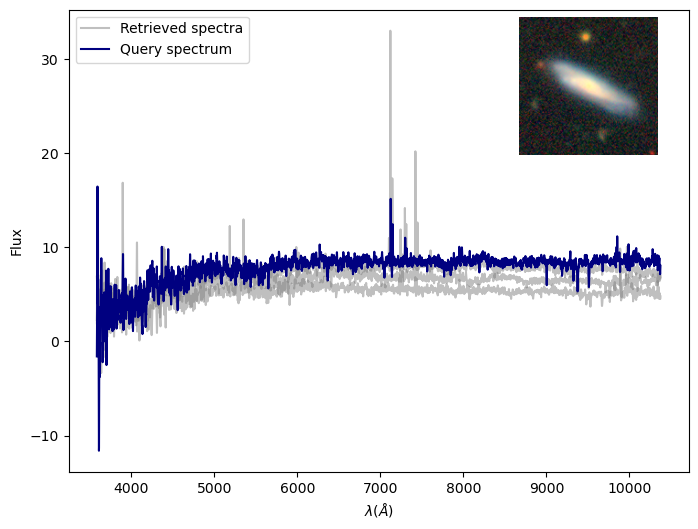
\includegraphics[width=\textwidth]{../figures/spectral_retrieval_im_sp_1}
        \caption{$S_C(\mathbf{z}_q^{\text{sp}}, \mathbf{z}_j^{\text{im}})$}
        \label{fig:im_sp_1}
    \end{subfigure}%
    \hfill
    \begin{subfigure}[b]{0.45\textwidth}
        \centering
        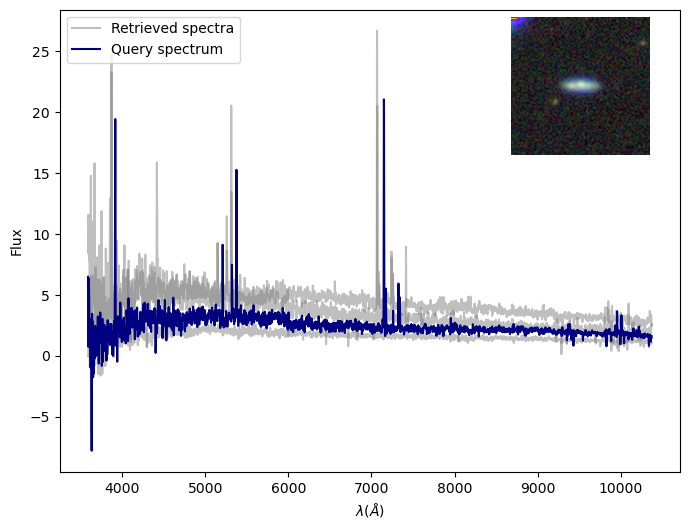
\includegraphics[width=\textwidth]{../figures/spectral_retrieval_im_sp_2}
        \caption{$S_C(\mathbf{z}_q^{\text{sp}}, \mathbf{z}_j^{\text{im}})$}
        \label{fig:im_sp_2}
    \end{subfigure}

    % Third row
    \begin{subfigure}[b]{0.45\textwidth}
        \centering
        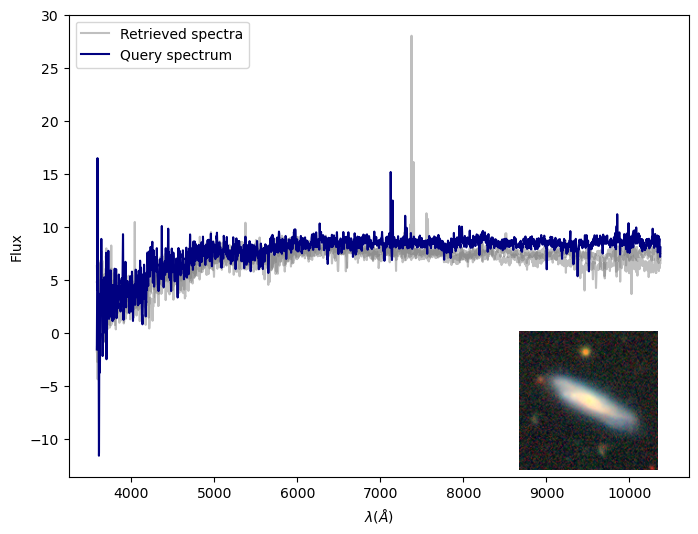
\includegraphics[width=\textwidth]{../figures/spectral_retrieval_sp_im_1}
        \caption{$S_C(\mathbf{z}_q^{\text{im}}, \mathbf{z}_j^{\text{sp}})$}
        \label{fig:sp_im_1}
    \end{subfigure}%
    \hfill
    \begin{subfigure}[b]{0.45\textwidth}
        \centering
        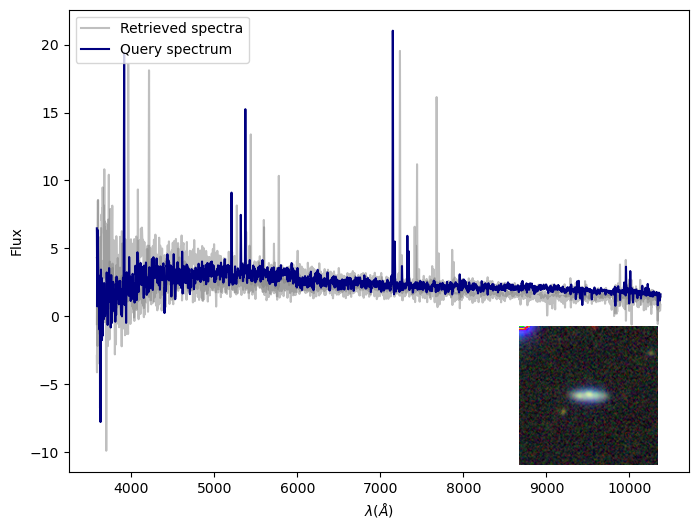
\includegraphics[width=\textwidth]{../figures/spectral_retrieval_sp_im_2}
        \caption{$S_C(\mathbf{z}_q^{\text{im}}, \mathbf{z}_j^{\text{sp}})$}
        \label{fig:sp_im_2}
    \end{subfigure}

    % Fourth row
    \begin{subfigure}[b]{0.45\textwidth}
        \centering
        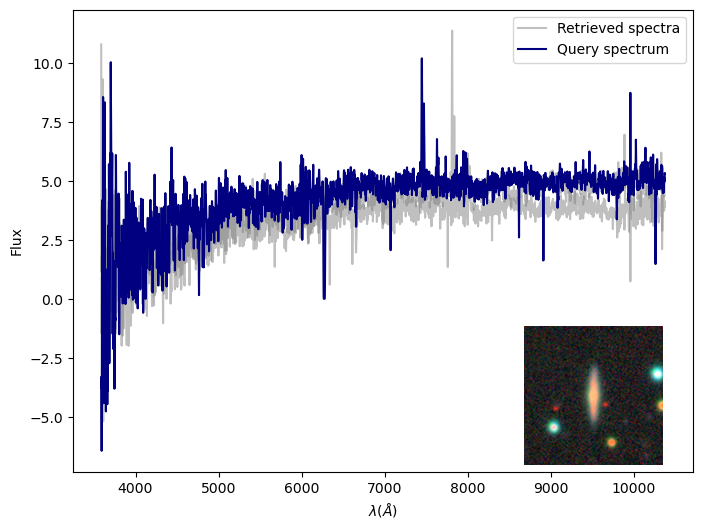
\includegraphics[width=\textwidth]{../figures/spectral_retrieval_sp_sp_1}
        \caption{$S_C(\mathbf{z}_q^{\text{sp}}, \mathbf{z}_j^{\text{sp}})$}
        \label{fig:sp_sp_1}
    \end{subfigure}%
    \hfill
    \begin{subfigure}[b]{0.45\textwidth}
        \centering
        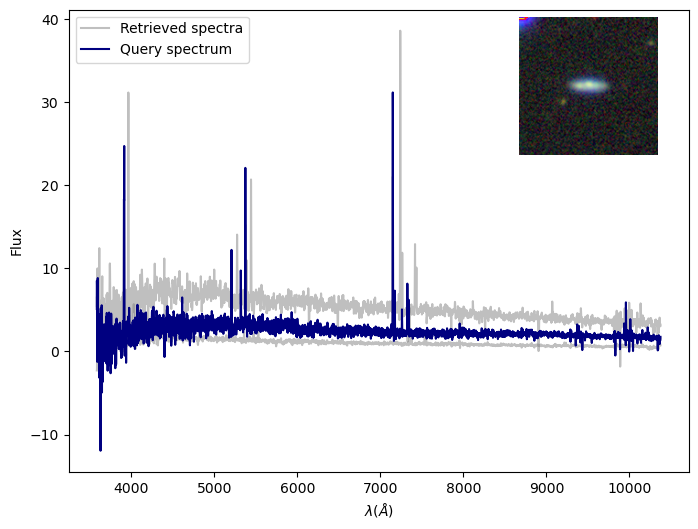
\includegraphics[width=\textwidth]{../figures/spectral_retrieval_sp_sp_2}
        \caption{$S_C(\mathbf{z}_q^{\text{sp}}, \mathbf{z}_j^{\text{sp}})$}
        \label{fig:sp_sp_2}
    \end{subfigure}

    % Add vertical space to extend into the bottom margin
    % \vspace*{-2cm}

    \caption{Spectral retrieval for query galaxies in the validation set. The top 5 most similar spectra are shown for each query galaxy in gray, while the query spectrum in shown in blue. The image of the query galaxy is shown in the corner of each plot.
    % . This was done using image-image search for (\ref{fig:im_im_1}) (\ref{fig:im_im_2}), image-spectrum search for (\ref{fig:im_sp_1}) (\ref{fig:im_sp_2}), spectrum-image search for (\ref{fig:sp_im_1}) (\ref{fig:sp_im_2}) and spectrum-spectrum search for (\ref{fig:sp_sp_1}) (\ref{fig:sp_sp_2}).
    }
    \label{fig:spectral_retrieval}
\end{figure}

This search retrieval ability can be useful in a variety of applications, such as seach for rare or unusual objects (see some examples of this in Ref.\cite{stein}). The results are largely consistent with the original work, although a direct comparison is difficult as the images and spectra chosen for queries are random. It is worth noting that our results are achieved using a much smaller model the original work, yet still yields (visually) similar results.

% \begin{figure}[H]
%     \centering
%     % First row
%     \begin{subfigure}[b]{0.45\textwidth}
%         \centering
%         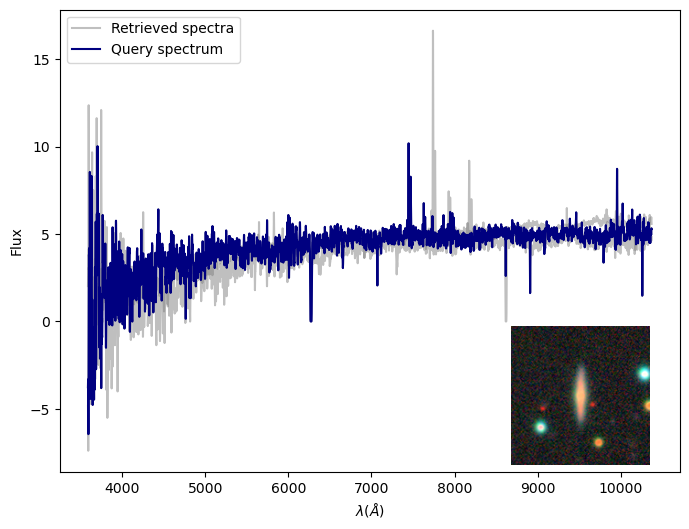
\includegraphics[width=\textwidth]{../figures/spectral_retrieval_im_im_1}
%         \caption{$S_C(\mathbf{z}_q^{\text{im}}, \mathbf{z}_j^{\text{im}})$}
%         \label{fig:im_im_1}
%     \end{subfigure}%
%     \hfill
%     \begin{subfigure}[b]{0.45\textwidth}
%         \centering
%         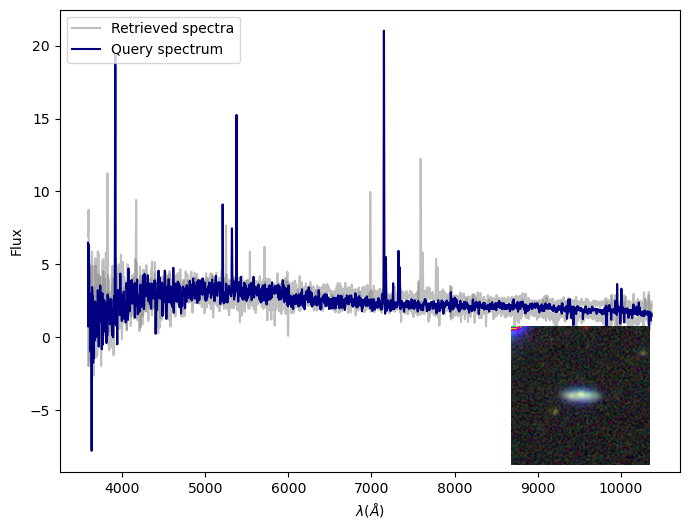
\includegraphics[width=\textwidth]{../figures/spectral_retrieval_im_im_2}
%         \caption{$S_C(\mathbf{z}_q^{\text{im}}, \mathbf{z}_j^{\text{im}})$}
%         \label{fig:im_im_2}
%     \end{subfigure}

%     % Second row
%     \begin{subfigure}[b]{0.45\textwidth}
%         \centering
%         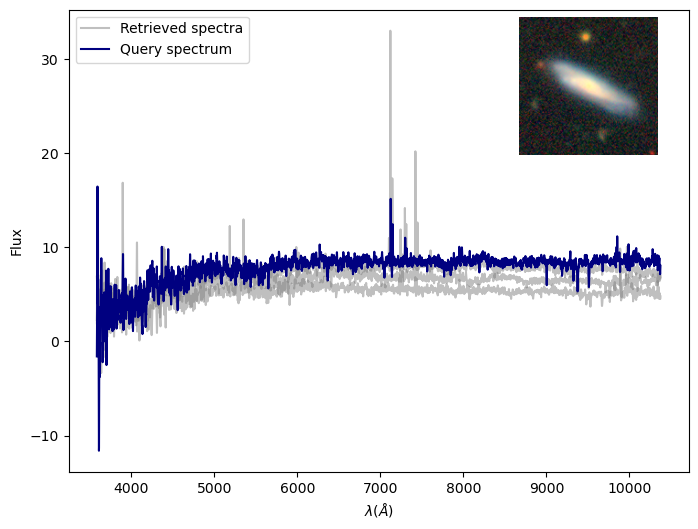
\includegraphics[width=\textwidth]{../figures/spectral_retrieval_im_sp_1}
%         \caption{$S_C(\mathbf{z}_q^{\text{sp}}, \mathbf{z}_j^{\text{im}})$}
%         \label{fig:im_sp_1}
%     \end{subfigure}%
%     \hfill
%     \begin{subfigure}[b]{0.45\textwidth}
%         \centering
%         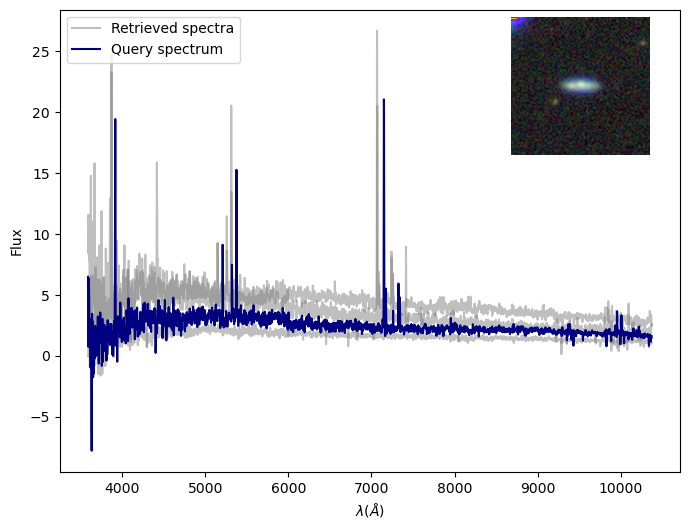
\includegraphics[width=\textwidth]{../figures/spectral_retrieval_im_sp_2}
%         \caption{$S_C(\mathbf{z}_q^{\text{sp}}, \mathbf{z}_j^{\text{im}})$}
%         \label{fig:im_sp_2}
%     \end{subfigure}

%     % Third row
%     \begin{subfigure}[b]{0.45\textwidth}
%         \centering
%         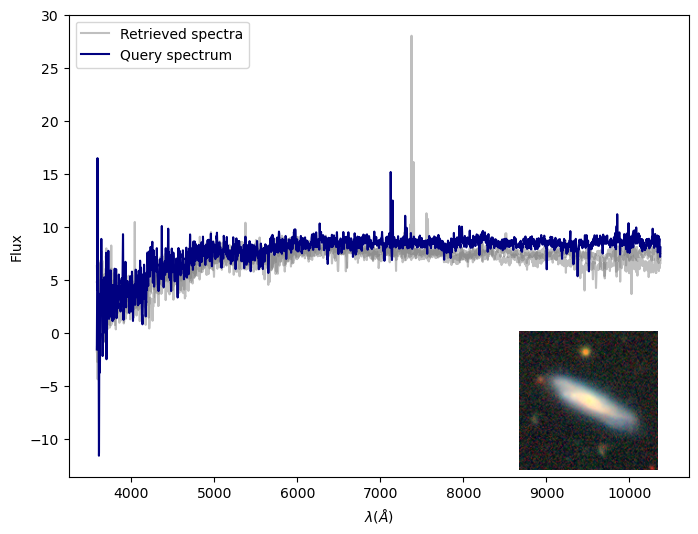
\includegraphics[width=\textwidth]{../figures/spectral_retrieval_sp_im_1}
%         \caption{$S_C(\mathbf{z}_q^{\text{im}}, \mathbf{z}_j^{\text{sp}})$}
%         \label{fig:sp_im_1}
%     \end{subfigure}%
%     \hfill
%     \begin{subfigure}[b]{0.45\textwidth}
%         \centering
%         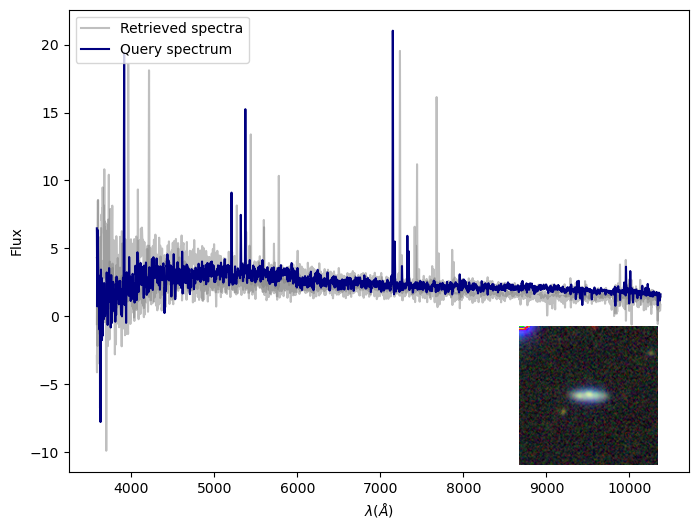
\includegraphics[width=\textwidth]{../figures/spectral_retrieval_sp_im_2}
%         \caption{$S_C(\mathbf{z}_q^{\text{im}}, \mathbf{z}_j^{\text{sp}})$}
%         \label{fig:sp_im_2}
%     \end{subfigure}

%     % Fourth row
%     \begin{subfigure}[b]{0.45\textwidth}
%         \centering
%         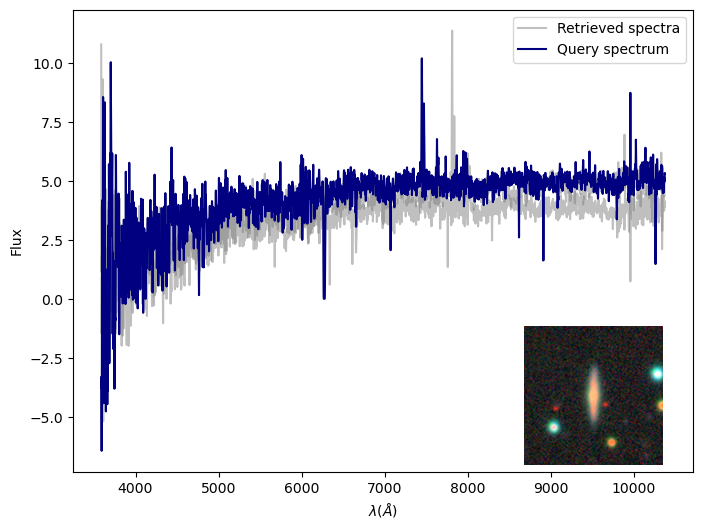
\includegraphics[width=\textwidth]{../figures/spectral_retrieval_sp_sp_1}
%         \caption{$S_C(\mathbf{z}_q^{\text{sp}}, \mathbf{z}_j^{\text{sp}})$}
%         \label{fig:sp_sp_1}
%     \end{subfigure}%
%     \hfill
%     \begin{subfigure}[b]{0.45\textwidth}
%         \centering
%         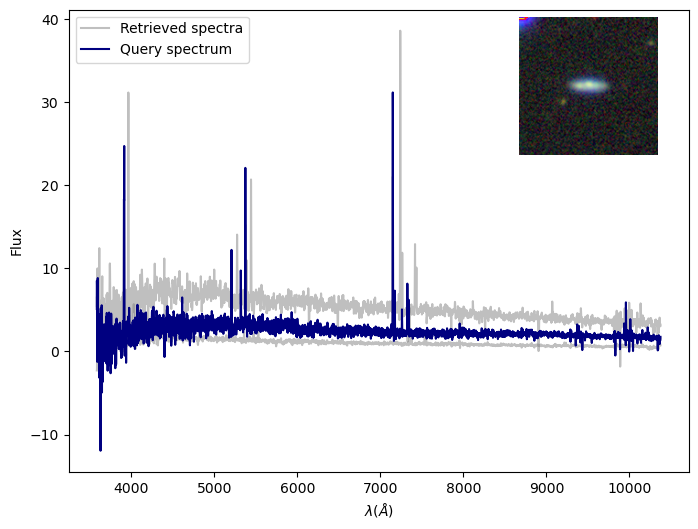
\includegraphics[width=\textwidth]{../figures/spectral_retrieval_sp_sp_2}
%         \caption{$S_C(\mathbf{z}_q^{\text{sp}}, \mathbf{z}_j^{\text{sp}})$}
%         \label{fig:sp_sp_2}
%     \end{subfigure}

%     \caption{Spectral retrieval for random query galaxies in the validation set. The top 5 most similar spectra are shown for each query galaxy, pictured in each graph. This was done using image-image search for (\ref{fig:im_im_1}) (\ref{fig:im_im_2}), image-spectrum search for (\ref{fig:im_sp_1}) (\ref{fig:im_sp_2}), spectrum-image search for (\ref{fig:sp_im_1}) (\ref{fig:sp_im_2}) and spectrum-spectrum search for (\ref{fig:sp_sp_1}) (\ref{fig:sp_sp_2}).}
%     \label{fig:spectral_retrieval}
% \end{figure}


\subsection{Zero Shot Prediction of Physical Properties}
We present the results of the zero-shot prediction of redshift and stellar mass in Fig.\ref{fig:zeroshot}. These plots depict a scatterplot of the $k$-NN redictions against the ProvaBGS catalogue values for the held-out set (grey points). A 2-D histogram is also plotted with a heatmap help to visualise the joint distribution of the two variables. Additionally, a Kernel Density Estimate (KDE) plot is used to overlay cotnour lines (in black) that represent levels of density over the scatter plot. The coefficient of determination $R^2$ score is also calculated for each prediction, which is a measure on the proportion of variance that is explained by the model. The $k$-NN regression is performed for both in-modality and cross-modality regression; for in-modality, we refer to case of using the same modality embeddings (image embeddings or spectrum embeddings) for both training and predicting the physical properties, while for cross-modality, we refer to the case of using spectrum embeddings for training and image embeddings for predicting. 

We can conclude that, similar to the original work, our embeddings give a strong zero-shot performance, indicating that the embedding space is able to organise itself around physically meaningful properties. The notably good performance even in the cross-modal case indicates that neighbours in the embedded space indeed share physically meaningful features regardless of the originating modality. Similar to the original work, the in-modality regression outperforms the cross-modality regression. This showcases that, although the constrastive loss aims to connect embeddings between modalities, this training objective causes the emergent property aiding in structuring the embeddings within respective modalities. Even though redshift was not an information explicitly used in the training, the spectrum-spectrum regression for redshift is able to capture a very high 0.87 of the variance in the data. This means that redshift has emerged as natural property to aid structure the embedding space.

Our reproduction results are consistent with the original work, but we note that we slightly underperform in all cases. This could be due to the smaller spectrum model used in our work. It could also be due to the model architecture itself, as the original work uses a transformer-based model which could capture a more nuanced representation of the spectra. Table \ref{tab:zeroshot} compares our results to the original work.


% Please add the following required packages to your document preamble:
% \usepackage{multirow}
\begin{table}[H]
    \begin{tabular}{clcc}
    \hline
    \textbf{Physical Property}    &                     & \begin{tabular}[c]{@{}c@{}}Original Work\\ $R^2$\end{tabular} & \begin{tabular}[c]{@{}c@{}}Our Reproduction\\ $R^2$\end{tabular} \\ \hline
    \hline
    \multirow{3}{*}{Redshift}     & Image Embeddings    & 0.71                                                          & 0.65                                                             \\
                                  & Spectrum Embeddings & 0.97                                                          & 0.87                                                             \\
                                  & Cross-Modal         & 0.64                                                          & 0.59                                                             \\ \hline
    \multirow{3}{*}{Stellar Mass} & Image Embeddings    & 0.66                                                          & 0.57                                                             \\
                                  & Spectrum Embeddings & 0.86                                                          & 0.74                                                             \\
                                  & Cross-Modal         & 0.58                                                          & 0.50                                                             \\ \hline
    \end{tabular}
    \caption{Comparison of $R^2$ scores for zero-shot prediction of redshift and stellar mass between the original AstroCLIP paper and our reproduction. By Cross-modal, we refer to the case of using spectrum embeddings for training of $k$-NN regression and image embeddings for prediction. For in-modality, we refer to the case of using the same modality embeddings for both training and prediction.}
    \label{tab:zeroshot}
\end{table}





\begin{figure}[H]
    \centering
    % Row 1: Image Embeddings
    \begin{subfigure}[b]{0.48\textwidth}
        \centering
        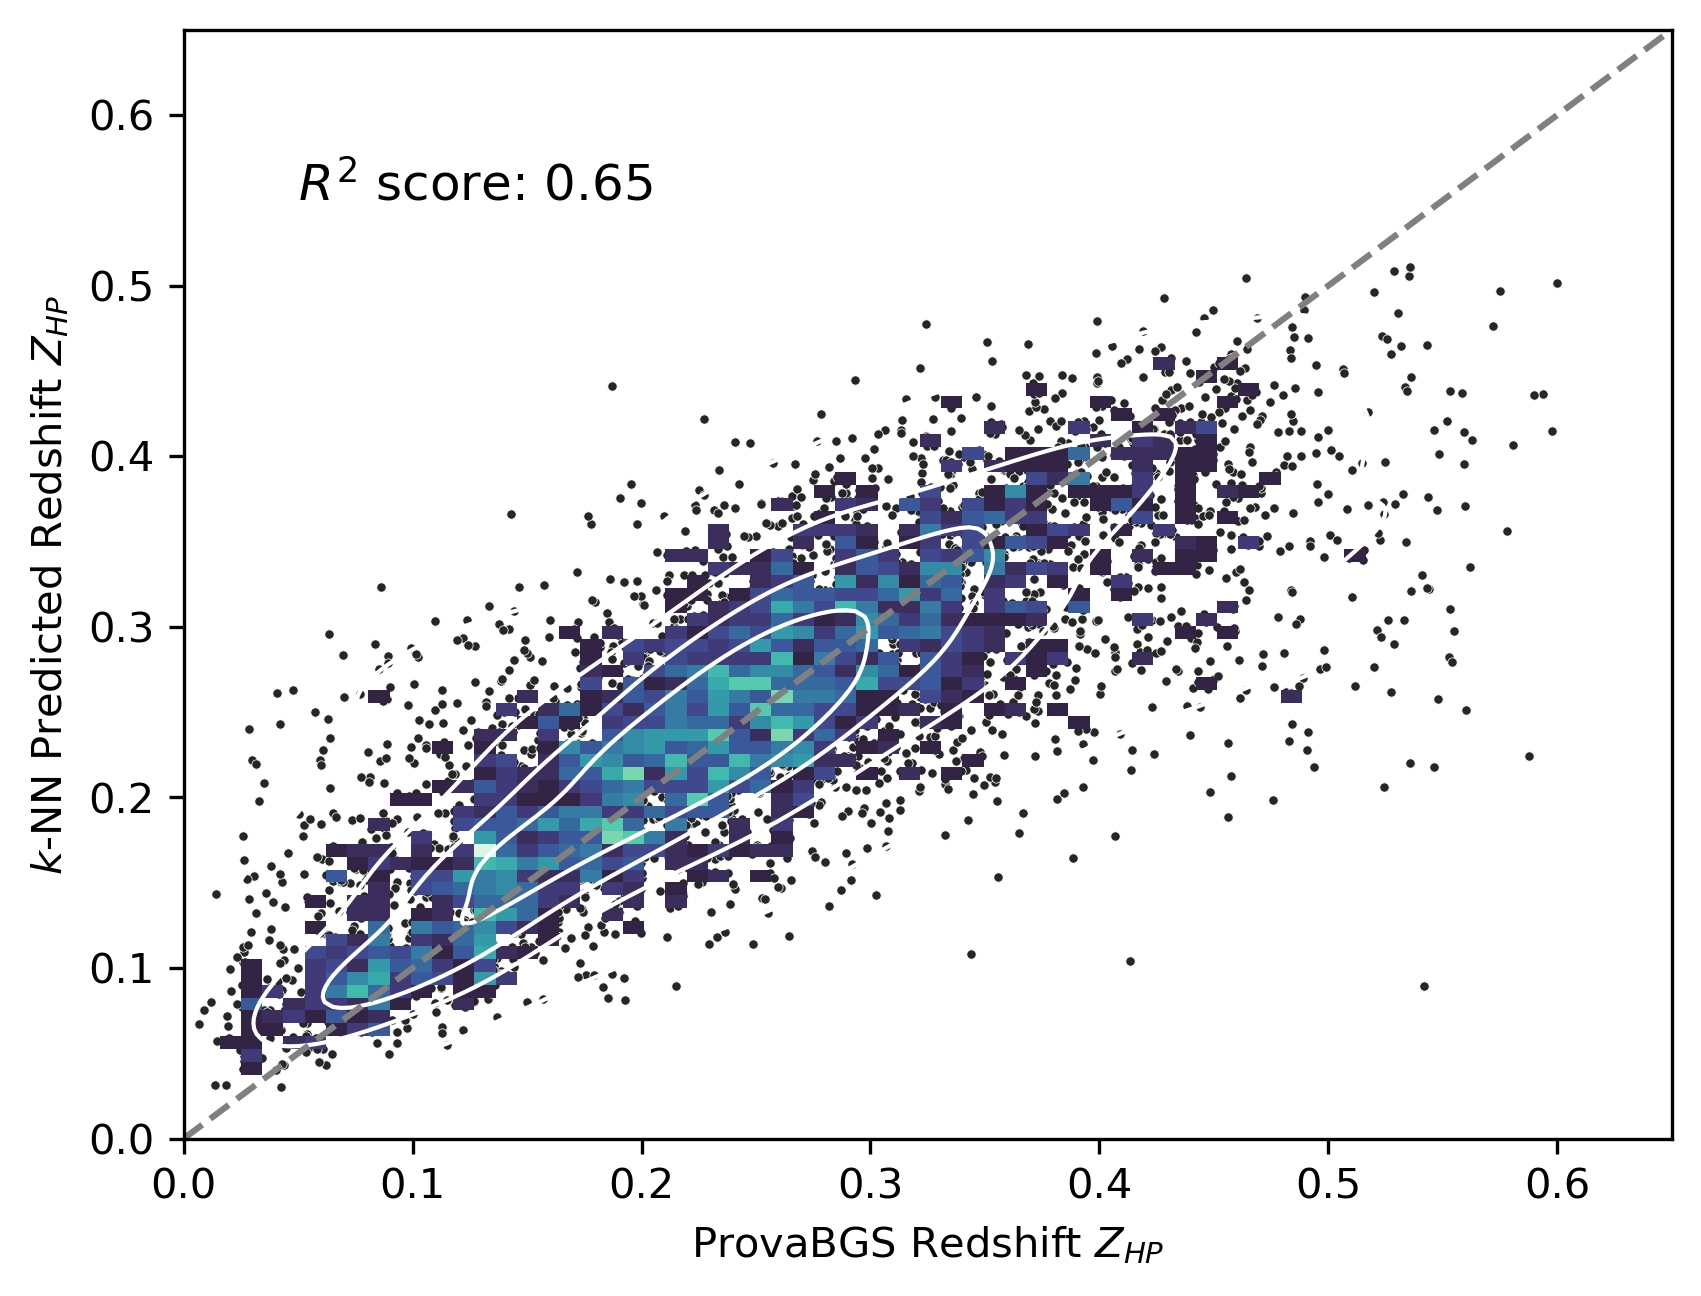
\includegraphics[width=\textwidth]{../figures/zeroshot_redshift_image.png}
        \caption{Image Embeddings for Redshift}
        \label{fig:redshift_image}
    \end{subfigure}%
    \hfill
    \begin{subfigure}[b]{0.48\textwidth}
        \centering
        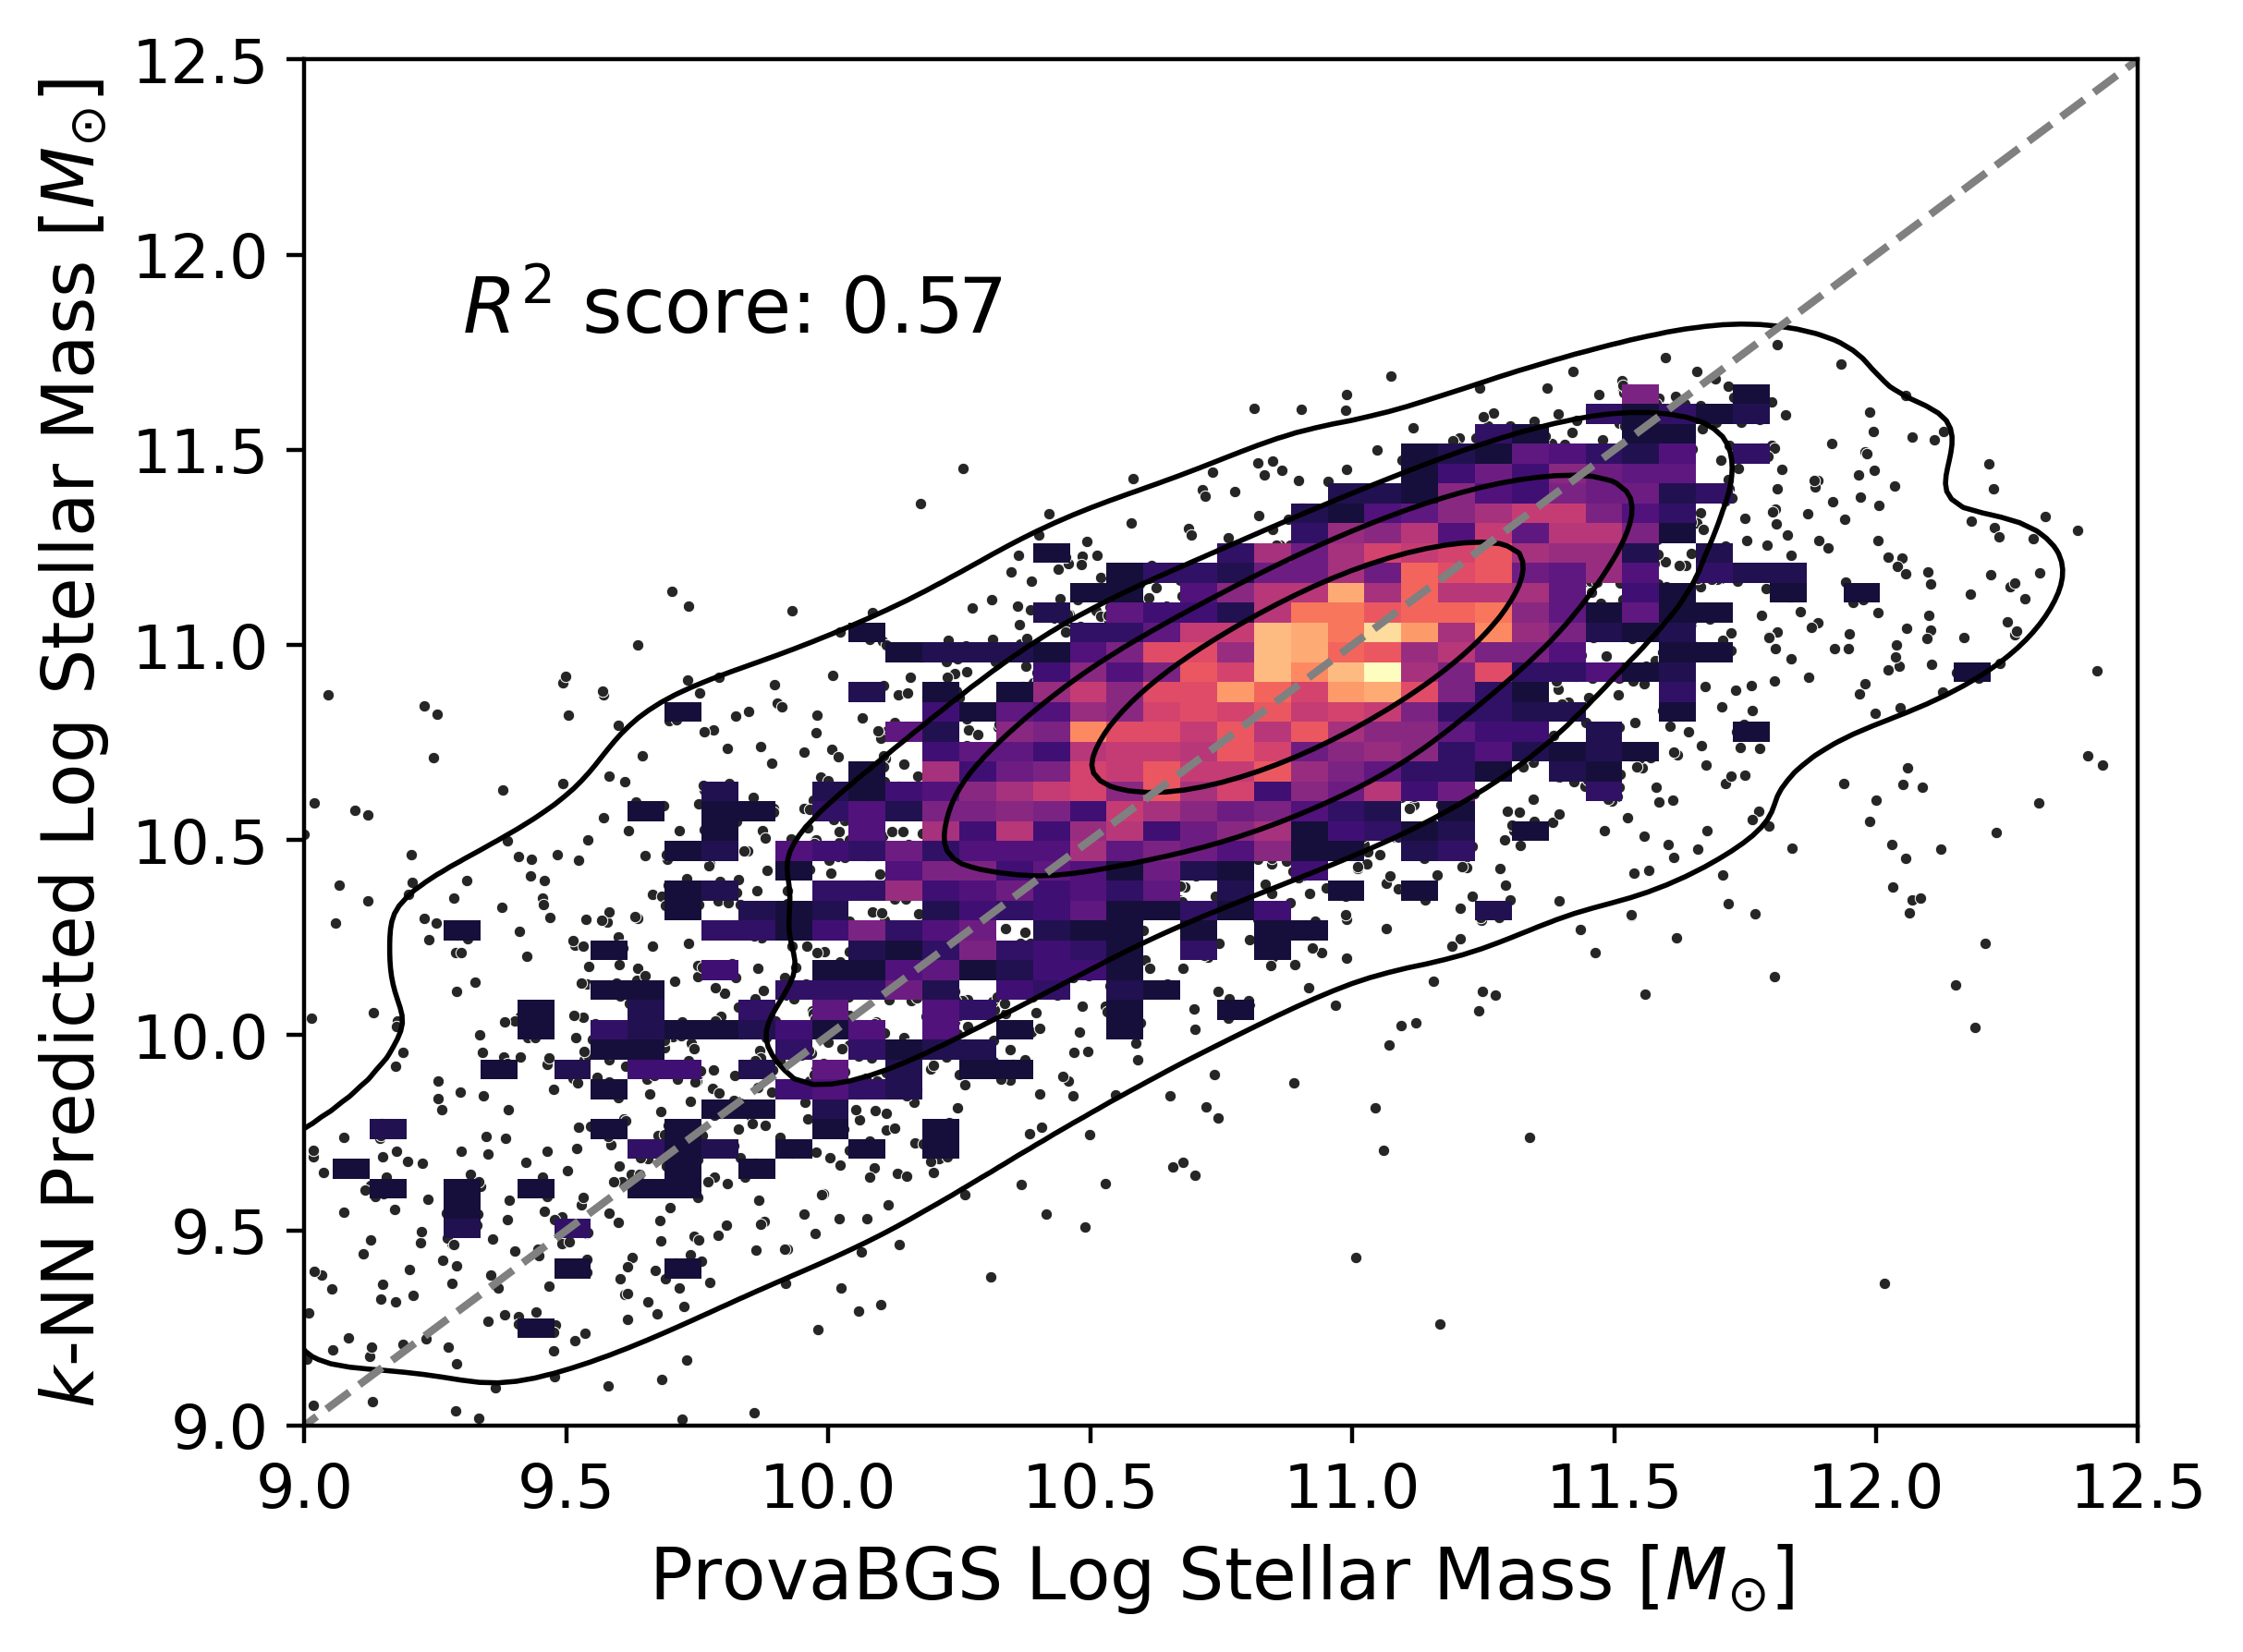
\includegraphics[width=\textwidth]{../figures/zeroshot_stellarmass_image.png}
        \caption{Image Embeddings for Stellar Mass}
        \label{fig:stellarmass_image}
    \end{subfigure}
    
    % Row 2: Spectrum Embeddings
    \begin{subfigure}[b]{0.48\textwidth}
        \centering
        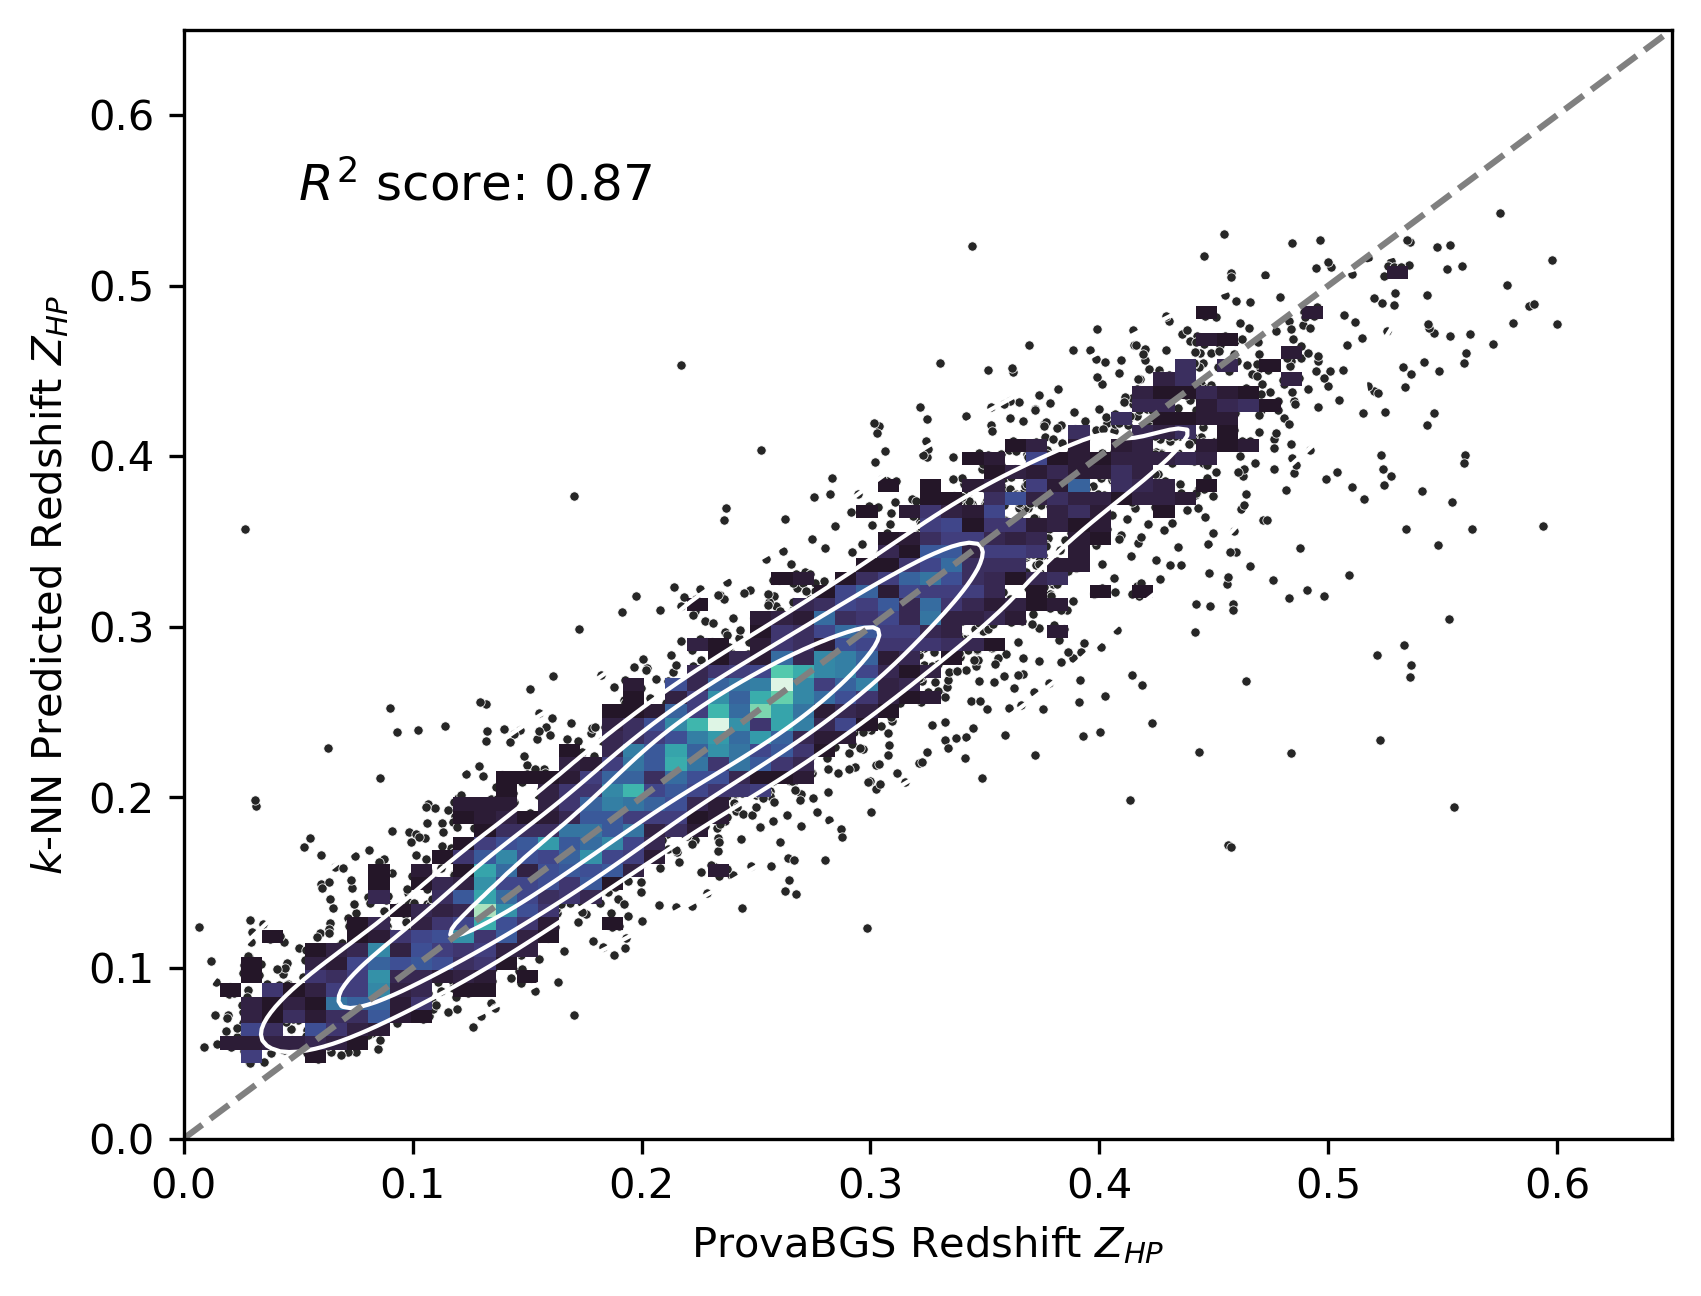
\includegraphics[width=\textwidth]{../figures/zeroshot_redshift_spectrum.png}
        \caption{Spectrum Embeddings for Redshift}
        \label{fig:redshift_spectrum}
    \end{subfigure}%
    \hfill
    \begin{subfigure}[b]{0.48\textwidth}
        \centering
        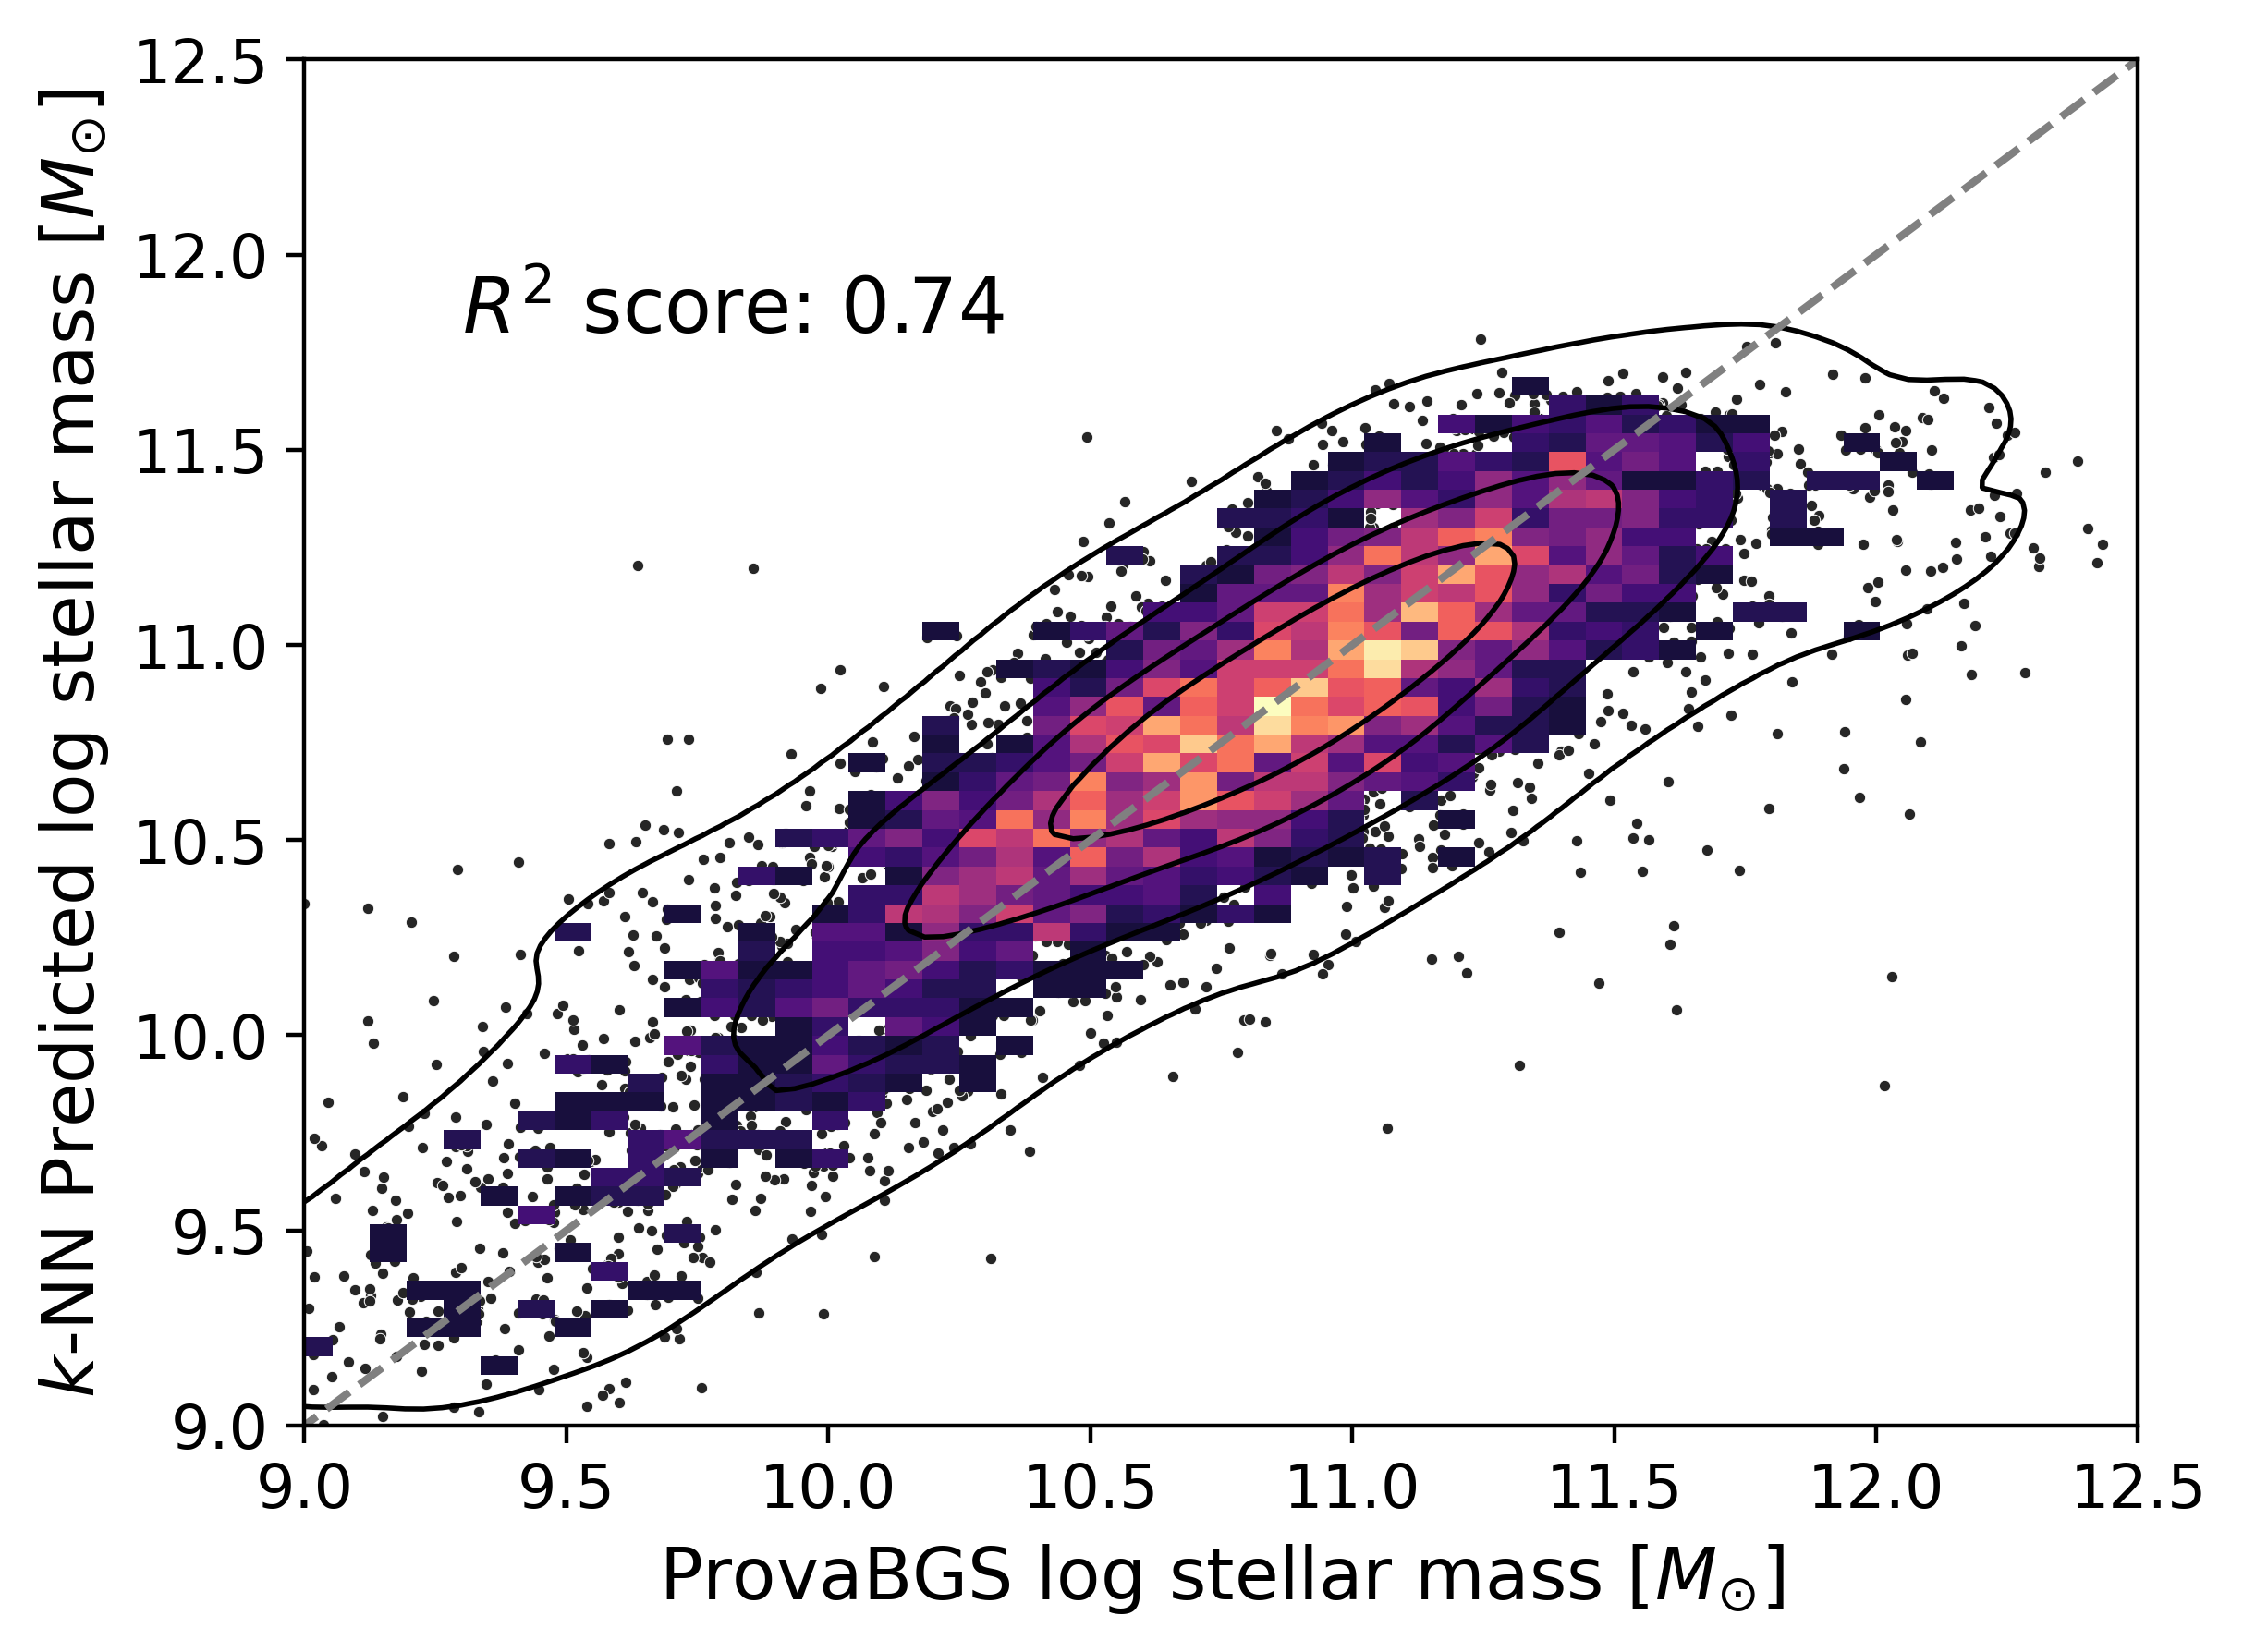
\includegraphics[width=\textwidth]{../figures/zeroshot_stellarmass_spectrum.png}
        \caption{Spectrum Embeddings for Stellar Mass}
        \label{fig:stellarmass_spectrum}
    \end{subfigure}

    % Row 3: Cross-Modal Embeddings
    \begin{subfigure}[b]{0.48\textwidth}
        \centering
        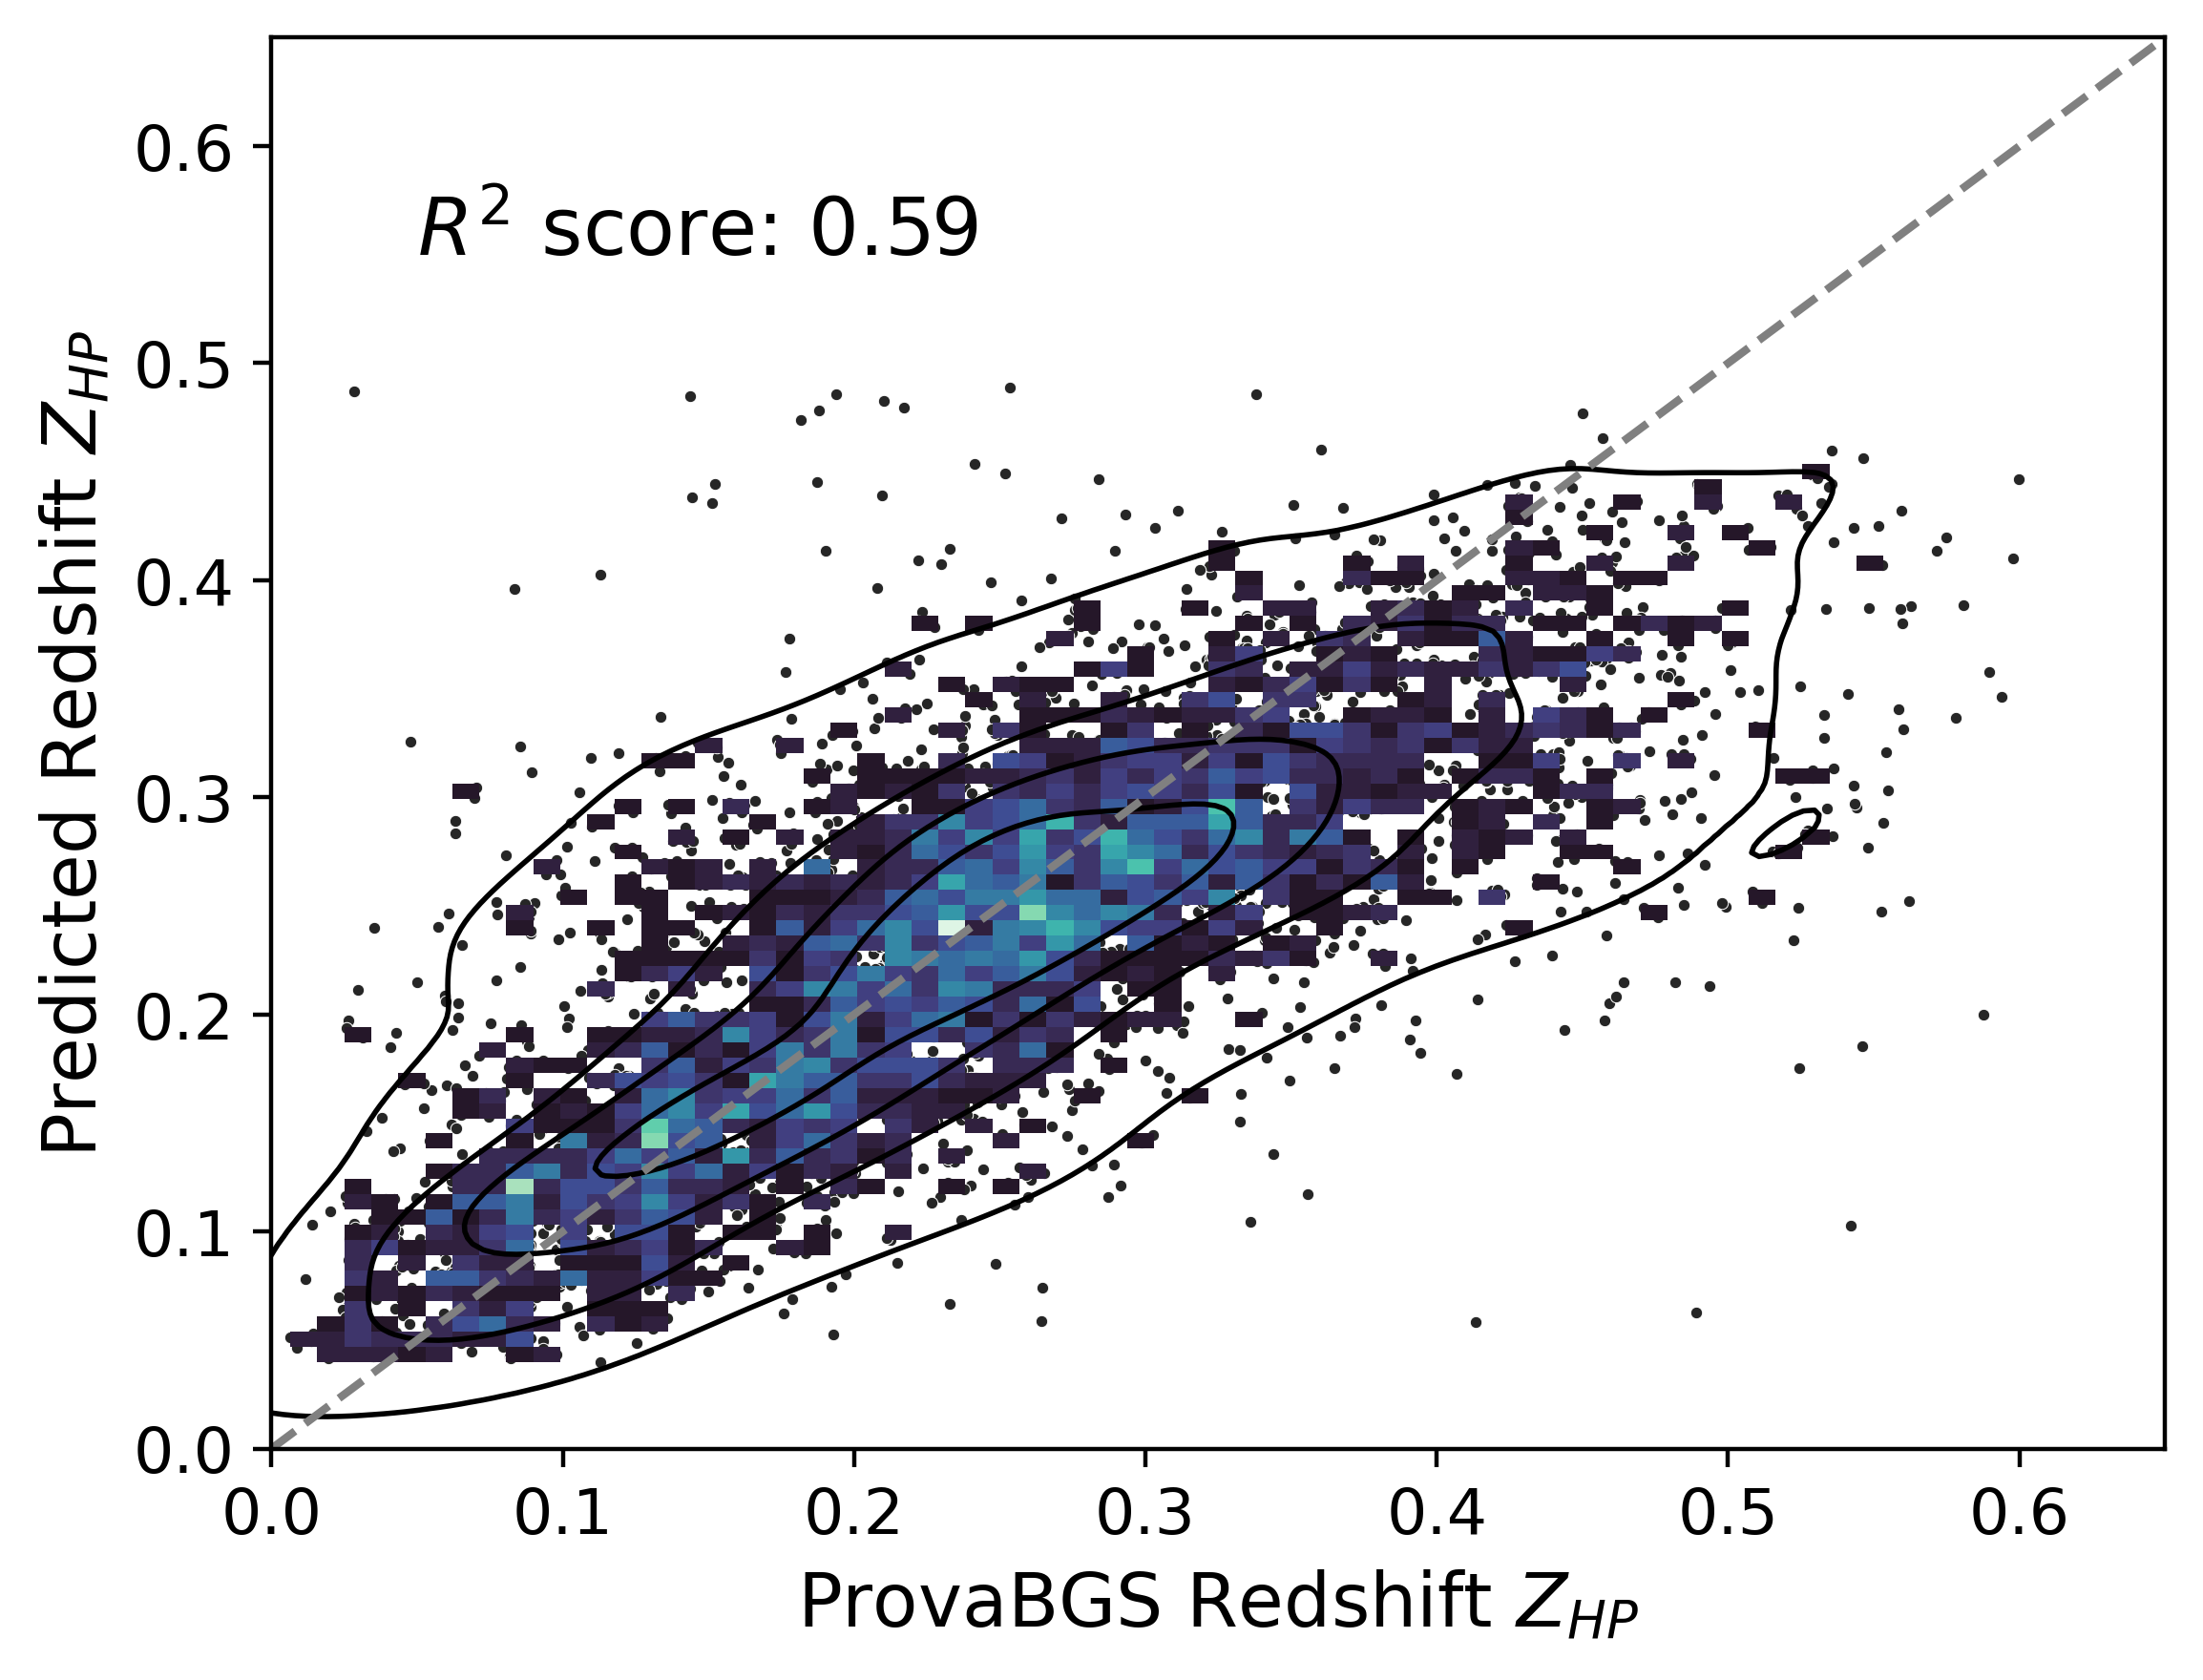
\includegraphics[width=\textwidth]{../figures/zeroshot_redshift_crossmodal.png}
        \caption{Cross-Modal Embeddings for Redshift}
        \label{fig:redshift_crossmodal}
    \end{subfigure}%
    \hfill
    \begin{subfigure}[b]{0.48\textwidth}
        \centering
        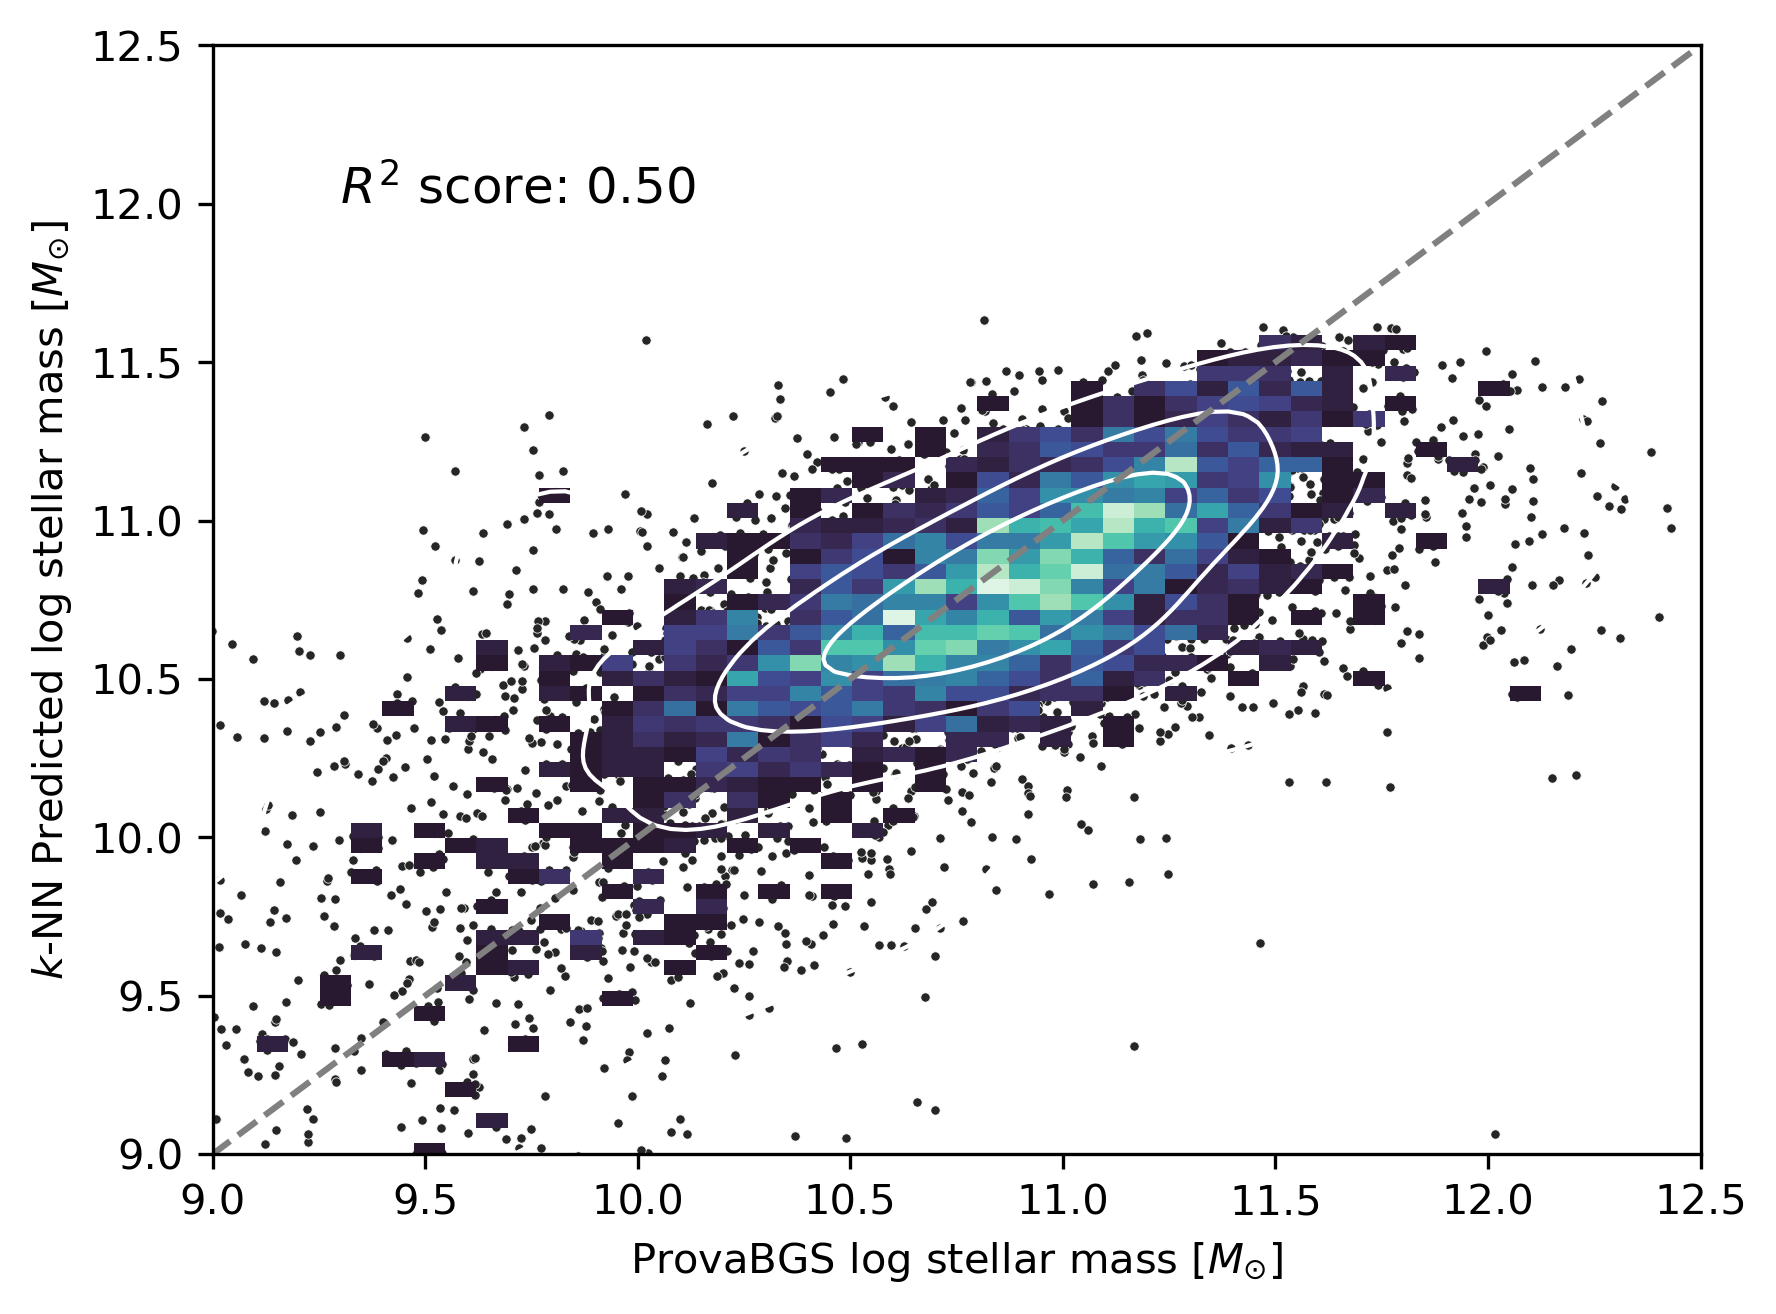
\includegraphics[width=\textwidth]{../figures/zeroshot_stellarmass_crossmodal.png}
        \caption{Cross-Modal Embeddings for Stellar Mass}
        \label{fig:stellarmass_crossmodal}
    \end{subfigure}

    \caption{Zero-shot prediction of redshift (left column) and stellar mass (right column) for the held-out set using $k$-NN regression purely on the embeddings. The results are shown for in-modal prediction using image embeddings (top row), spectrum embeddings (middle row), and cross-modal prediction using spectrum embeddings for training and image embeddings for prediction (bottom row). On the $x$-axis we plot the PROVABGS catalogue values as ground truth, and on the $y$-axis we plot the $k$-NN predictions. A perfect prediction would lie on the diagonal line $ y = x $. The $R^2$ score is calculated for each prediction and is annotated in the top right corner of each plot.}
    \label{fig:zeroshot}
\end{figure}



\subsection{Embedding Space Clustering}
As an extension to the original work, we visualise the embedding space and subsequently use clustering techniques to further examine how the model structures the data. Fig.\ref{fig:umap_of_spectra} shows the UMAP projection of the spectrum embeddings, coloured by their catalogued redshift values $Z_{HP}$ on the left and stellar mass values $M_{\star}$ on the right. The projection reveals a clear structure, where low redshift galaxies are clustered in the lower left corner, rising to higher redshifts as we move to the upper right corner. The same pattern is present in the stellar mass plot. This again illustrates the emergent behaviour of the model to structure the embedding space around physically meaningful properties, despite not being explicitly trained on these properties. 


\begin{figure}[H]
    \centering
    \begin{adjustbox}{addcode={
      \begin{minipage}{\width}}{
      \end{minipage}},rotate=0,center}
      \includegraphics[width=1.15\textwidth]{../figures/umap_spectra_heatmap.png} % 1.3x text width to extend into the margins
    \end{adjustbox}
    \caption{\textbf{Spectrum embeddings} UMAP projection coloured by redshift $Z_{HP}$ (left) and stellar mass $M_{\star}$ (right). The projection reveals a clear structure for both projections, where low redshift and stellar mass galaxies are clustered in the lower left corner, rising to higher values as we move to the upper right corner.}
    \label{fig:umap_of_spectra}
\end{figure}

\begin{figure}[H]
    \centering
    \begin{adjustbox}{addcode={
      \begin{minipage}{\width}}{
      \end{minipage}},rotate=0,center}
      \includegraphics[width=1.15\textwidth]{../figures/umap_image_heatmap.png} % 1.3x text width to extend into the margins
    \end{adjustbox}
    \caption{\textbf{Image embeddings} UMAP projection coloured by redshift $Z_{HP}$ (left) and stellar mass $M_{\star}$ (right). The projection reveals a clear structure for both projections, where low redshift and stellar mass galaxies are clustered in the lower left corner, rising to higher values as we move to the upper right corner.}
    \label{fig:umap_of_images}
\end{figure}


\begin{figure}[H]
    \centering
    \begin{adjustbox}{addcode={
      \begin{minipage}{\width}}{
      \end{minipage}},rotate=0,center}
      \includegraphics[width=1.15\textwidth]{../figures/umap_both_heatmap.png}
    \end{adjustbox}
    \caption{ \textbf{Combined image-spectrum embeddings} UMAP projection coloured by redshift $Z_{HP}$ (left) and stellar mass $M_{\star}$ (right). The projection reveals a clear structure for both projections, where high redshift and stellar mass galaxies are clustered in the lower left corner, falling to lower values as we move to the upper right corner.}
    \label{fig:umap_of_both}
\end{figure}

Fig.\ref{fig:umap_of_images} and Fig.\ref{fig:umap_of_both} show the UMAP projection of the image embeddings and the combined image-spectrum embeddings, respectively. Similarly to the spectrum embeddings, we again see this clear structuring in the embedding space, with one difference: these mapping include a large `island' of galaxies that does not contain particular property values. Rather, it largely follows a similar pattern to the main `island', indicating this break-off is caused by some other property.


% To further examine this and other potential islands, we use DBScan to directly cluster the UMAP projection. The clusters are illustrated in Fig.\ref{fig:umap_DBSCAN}

% \begin{figure}[H]
%     \centering
%     \begin{adjustbox}{addcode={
%       \begin{minipage}{\width}}{
%       \end{minipage}},rotate=0,center}
%       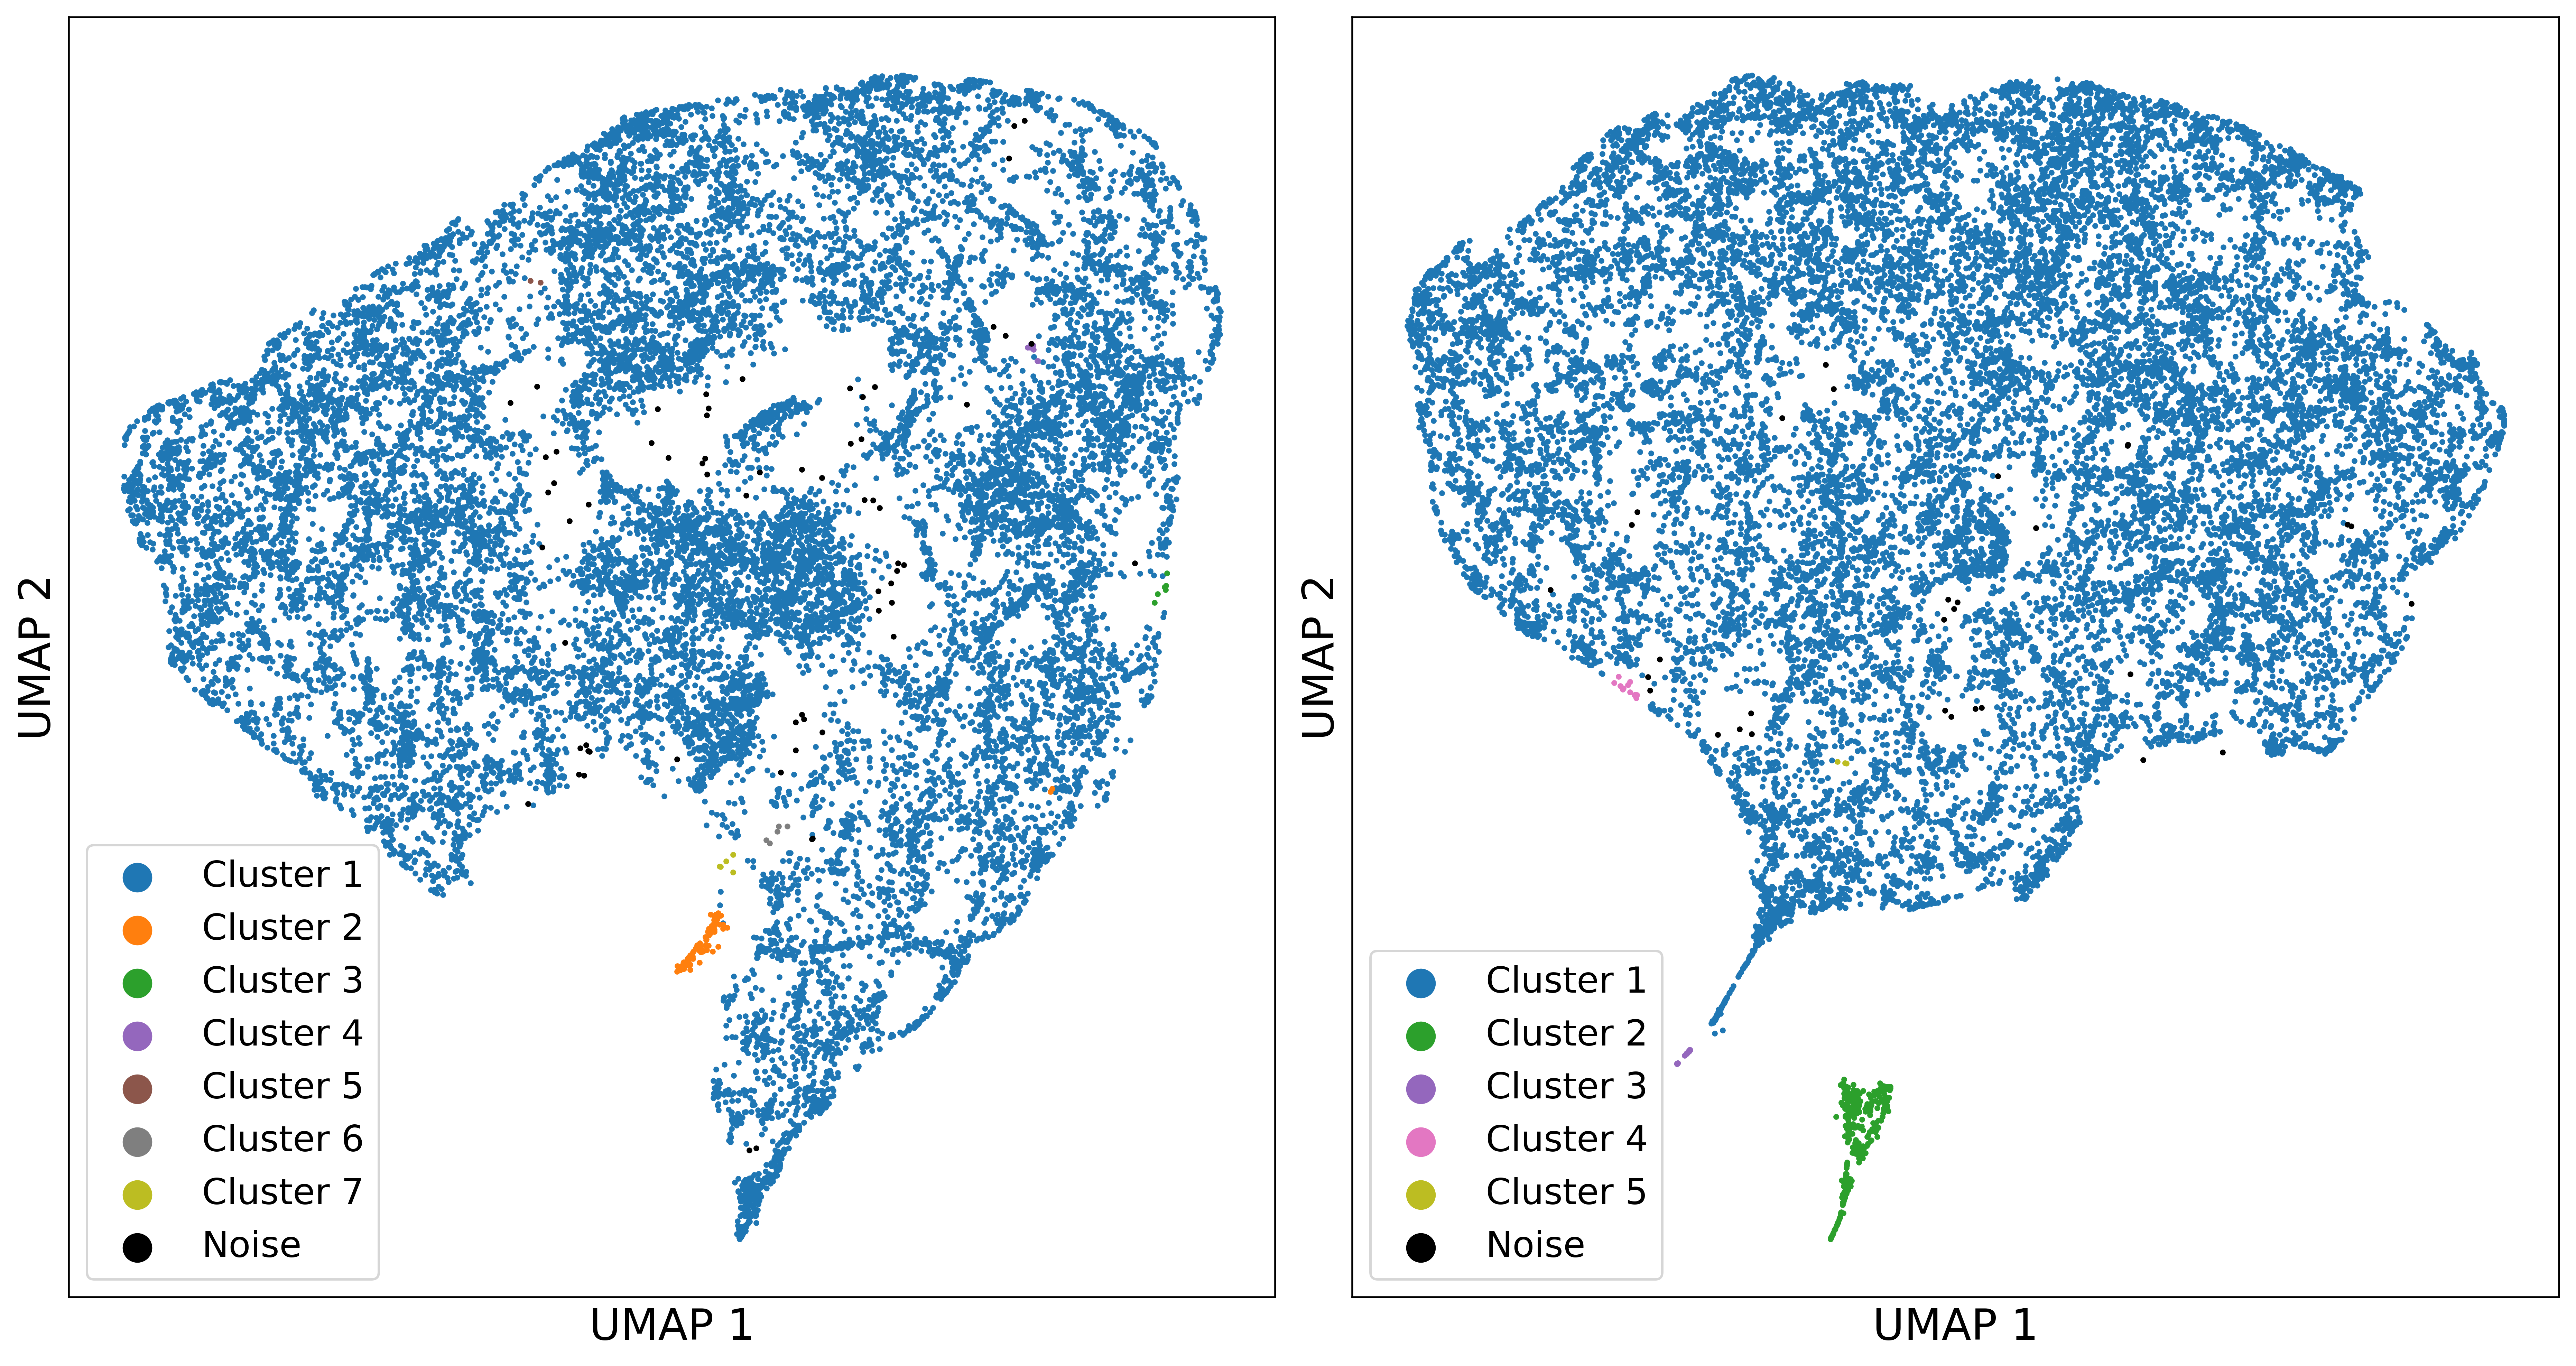
\includegraphics[width=1.15\textwidth]{../figures/umap_dbscan_clusters.png}
%     \end{adjustbox}
%     \caption{UMAP projection of the spectrum embeddings (left) and image embeddings (right) coloured by the DBScan clustering.}
%     \label{fig:umap_DBSCAN}
% \end{figure}

To further examine this and other potential islands, we use DBSCAN to directly cluster the UMAP projection of the image embeddings. We set $\epsilon = 0.20$ and the minimum number of samples to 5. These were chosen by trial and error to produce a reasonable number of clusters in both the image and spectrum embeddings, with a reasonable number of galaxies in each. We then draw sample galaxies for each cluster to visually inspect. The clusters for the image embeddings are illustrated in Fig.\ref{fig:umap_DBSCAN}.

The clustering reveals that the image embedder has successfully separated galaxy images that contain artifacts caused by the image capture process to a distinct embedding island (Cluster 2). The galaxies contained in those images have variable redshifts and stellar masses, and are follow the same distribution as the main island. This is potentially a useful feature for quickly identifying artifacts in galaxy catalogues. We further display 3 more islands: cluster 3 and 4 contain galaxies that largely fill the image, are mostly spiral and have high brightness. This indicates that model is able to separate galaxies based on their morphology, which is a key feature in galaxy classification. 

It is important to note that although we visualise image embeddings in isolation, their structure is informed by the spectrum embeddings during training, which means that it contains information about the galaxy's spectrum as well. This also true for the spectrum embeddings, which are informed by the image embeddings. We make this statement more concrete by showcasing the results of $k$-Means clustering on the full dimensional space of just the spectrum embeddings. Here, we first perform the clustering and then project the clusters onto the UMAP projection of the spectrum embeddings. We choose to use 10 clusters, as they yield a reasonable silhouette score and a reasonable number of galaxies in each cluster. 


\begin{figure}[H]
    \centering
    \begin{adjustbox}{addcode={
      \begin{minipage}{\width}}{
      \end{minipage}},rotate=0,center}
      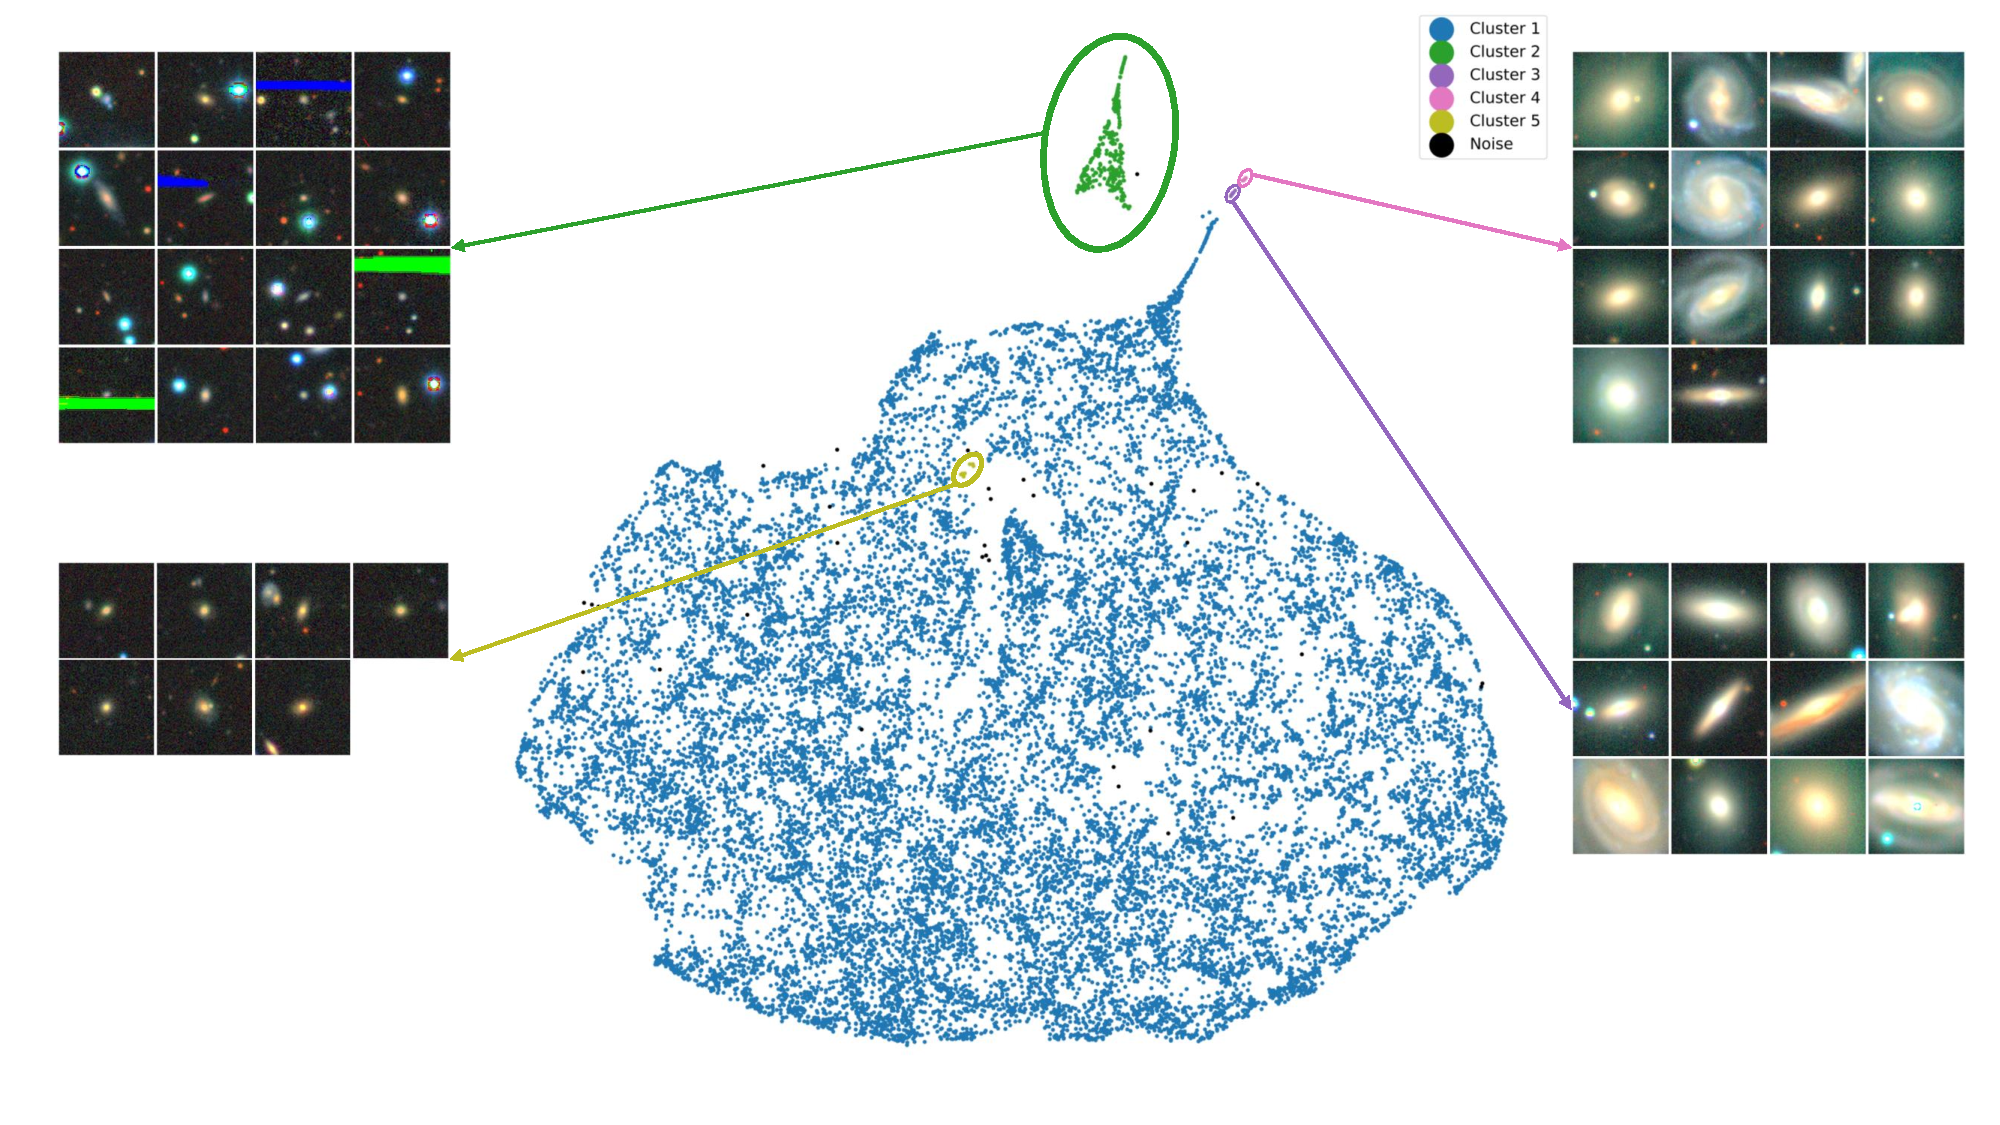
\includegraphics[width=1.15\textwidth]{../figures/dbscan_image_clusters_shown.pdf}
    \end{adjustbox}
    \caption{UMAP projection of the image embeddings coloured by the DBScan clustering. We show the images of samples of the largest island cluster (top left), and all the galaxy images contained in clusters 3, 4 and 5.}
    \label{fig:umap_DBSCAN}
\end{figure}


We then visualise a random sample of the spectra in each cluster, as shown in Fig.\ref{fig:annotated_spectra}. We observe that galaxies in the same cluster follow similar trends in their spectra, both in terms of the overall shape, the presense of specific spectral features and the flux range and scale. In addition to this we show that not only are the spectra in the same cluster similar, but the images of the galaxies are also visually similar, as shown in Fig.\ref{fig:annotated_images}. Recall that we are only considering the spectrum embeddings in this case, which means that the model has learned to structure the spectrum embeddings in a way that is informed by the image embeddings. This is a key feature of the AstroCLIP model, as it allows for the alignment of the two modalities in the shared latent space. Furthermore, it reveals a potential capability of the model to cluster the embeddings based on morphology, which is a key feature in galaxy classification. 

A noteworthy feature of this latest UMAP projection a distinct ring of galaxies on the main island that is permeating into different clusters. This could be an interesting feature to investigate further, as it could be indicative of a specific physical property that is not captured by the redshift or stellar mass.


\begin{figure}[H]
    \centering
    \vspace{-1cm}
    \begin{adjustbox}{addcode={
      \begin{minipage}{\width}}{
      \end{minipage}},rotate=0,center}
      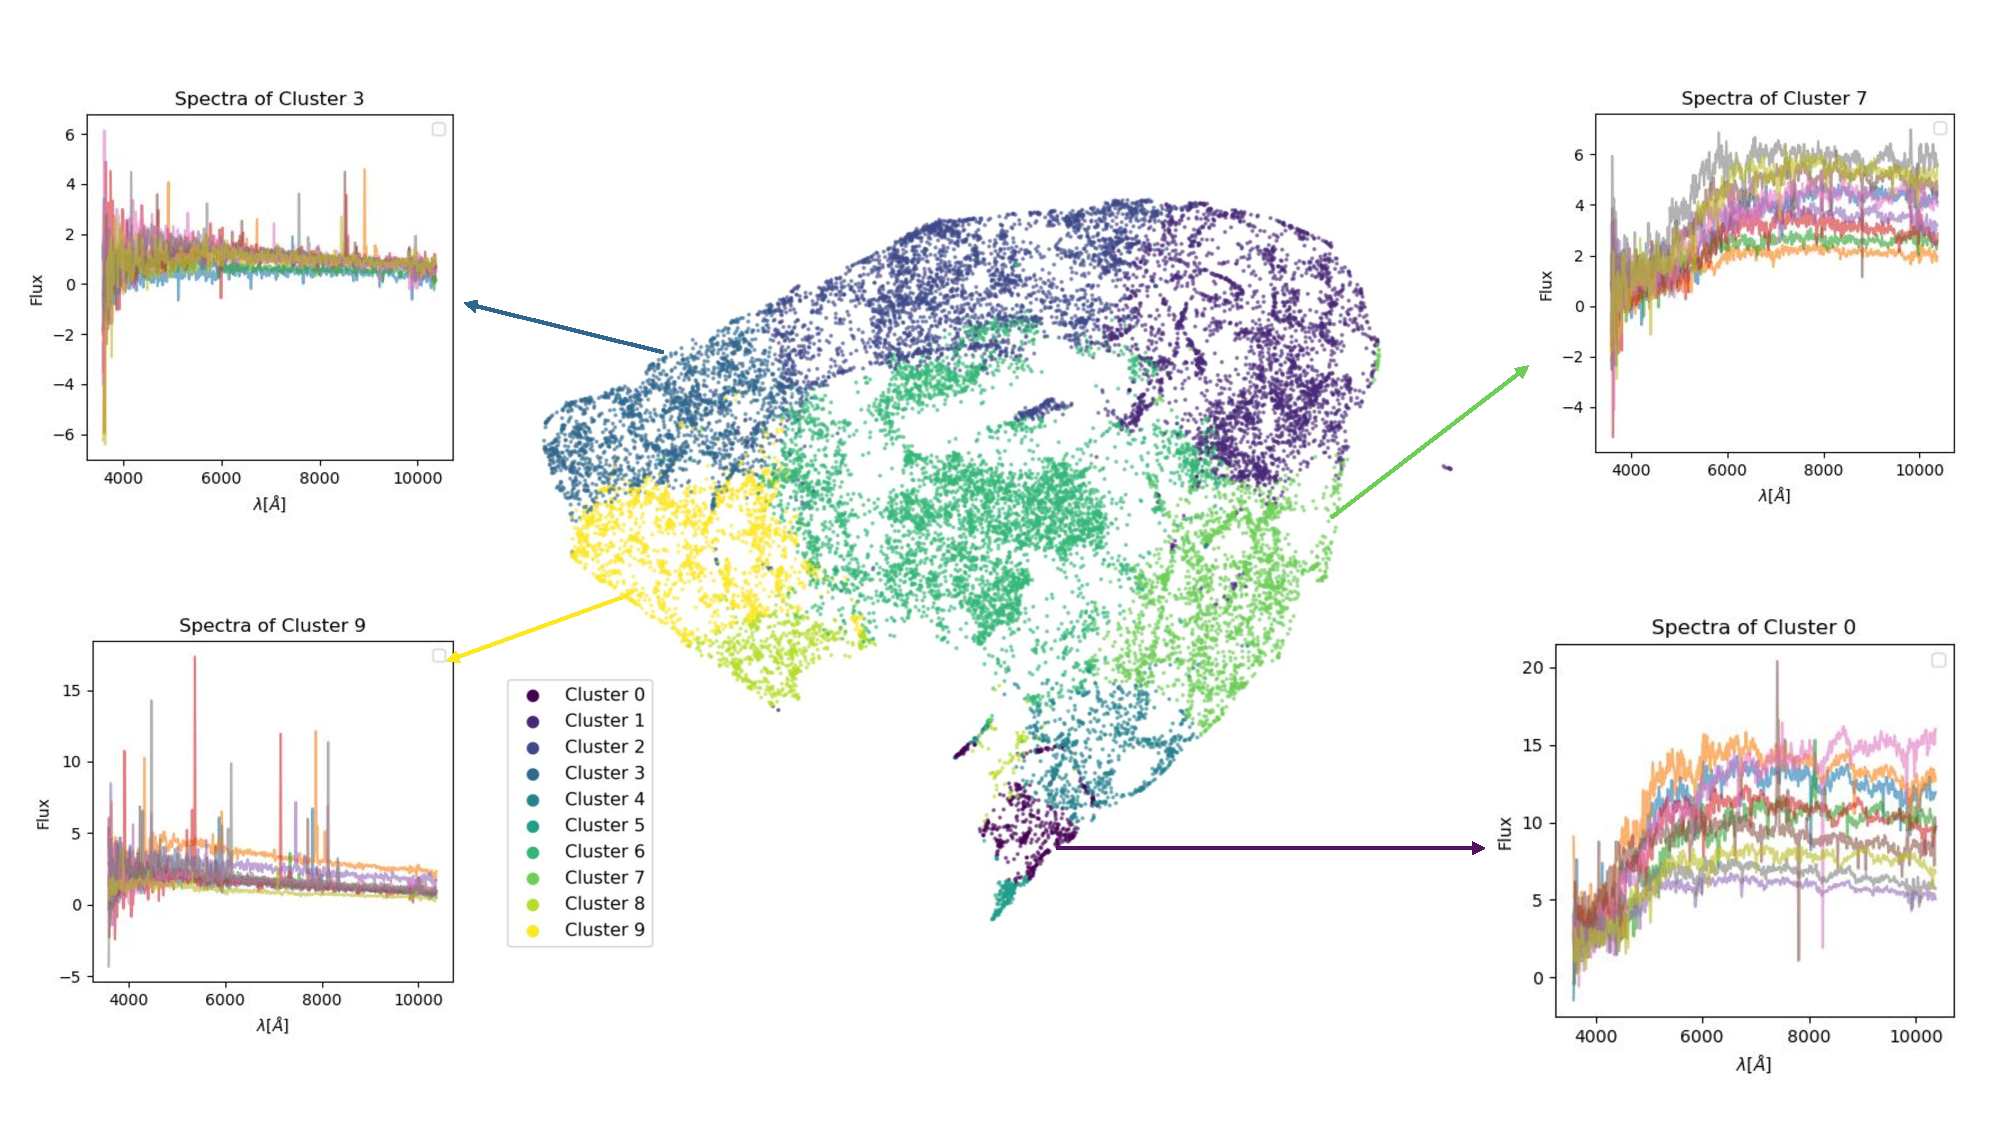
\includegraphics[width=1.15\textwidth]{../figures/umap_spectrum_annotated_spectra.pdf}
    \end{adjustbox}
    \caption{UMAP projection of the spectrum embeddings coloured by the $k$-Means clustering. The spectra of random samples from clusters [0,3,7,9] are shown in the four corners of this plot. The colours in the spectrum plots correspond to different galaxies within the specified spectrum (they are not related to the cluster colouring). All spectra follow similar trends in their shape within their respective clusters in terms of colour and shape.}
    \label{fig:annotated_spectra}
\end{figure}

\begin{figure}[H]
    \centering
    \begin{adjustbox}{addcode={
      \begin{minipage}{\width}}{
      \end{minipage}},rotate=0,center}
      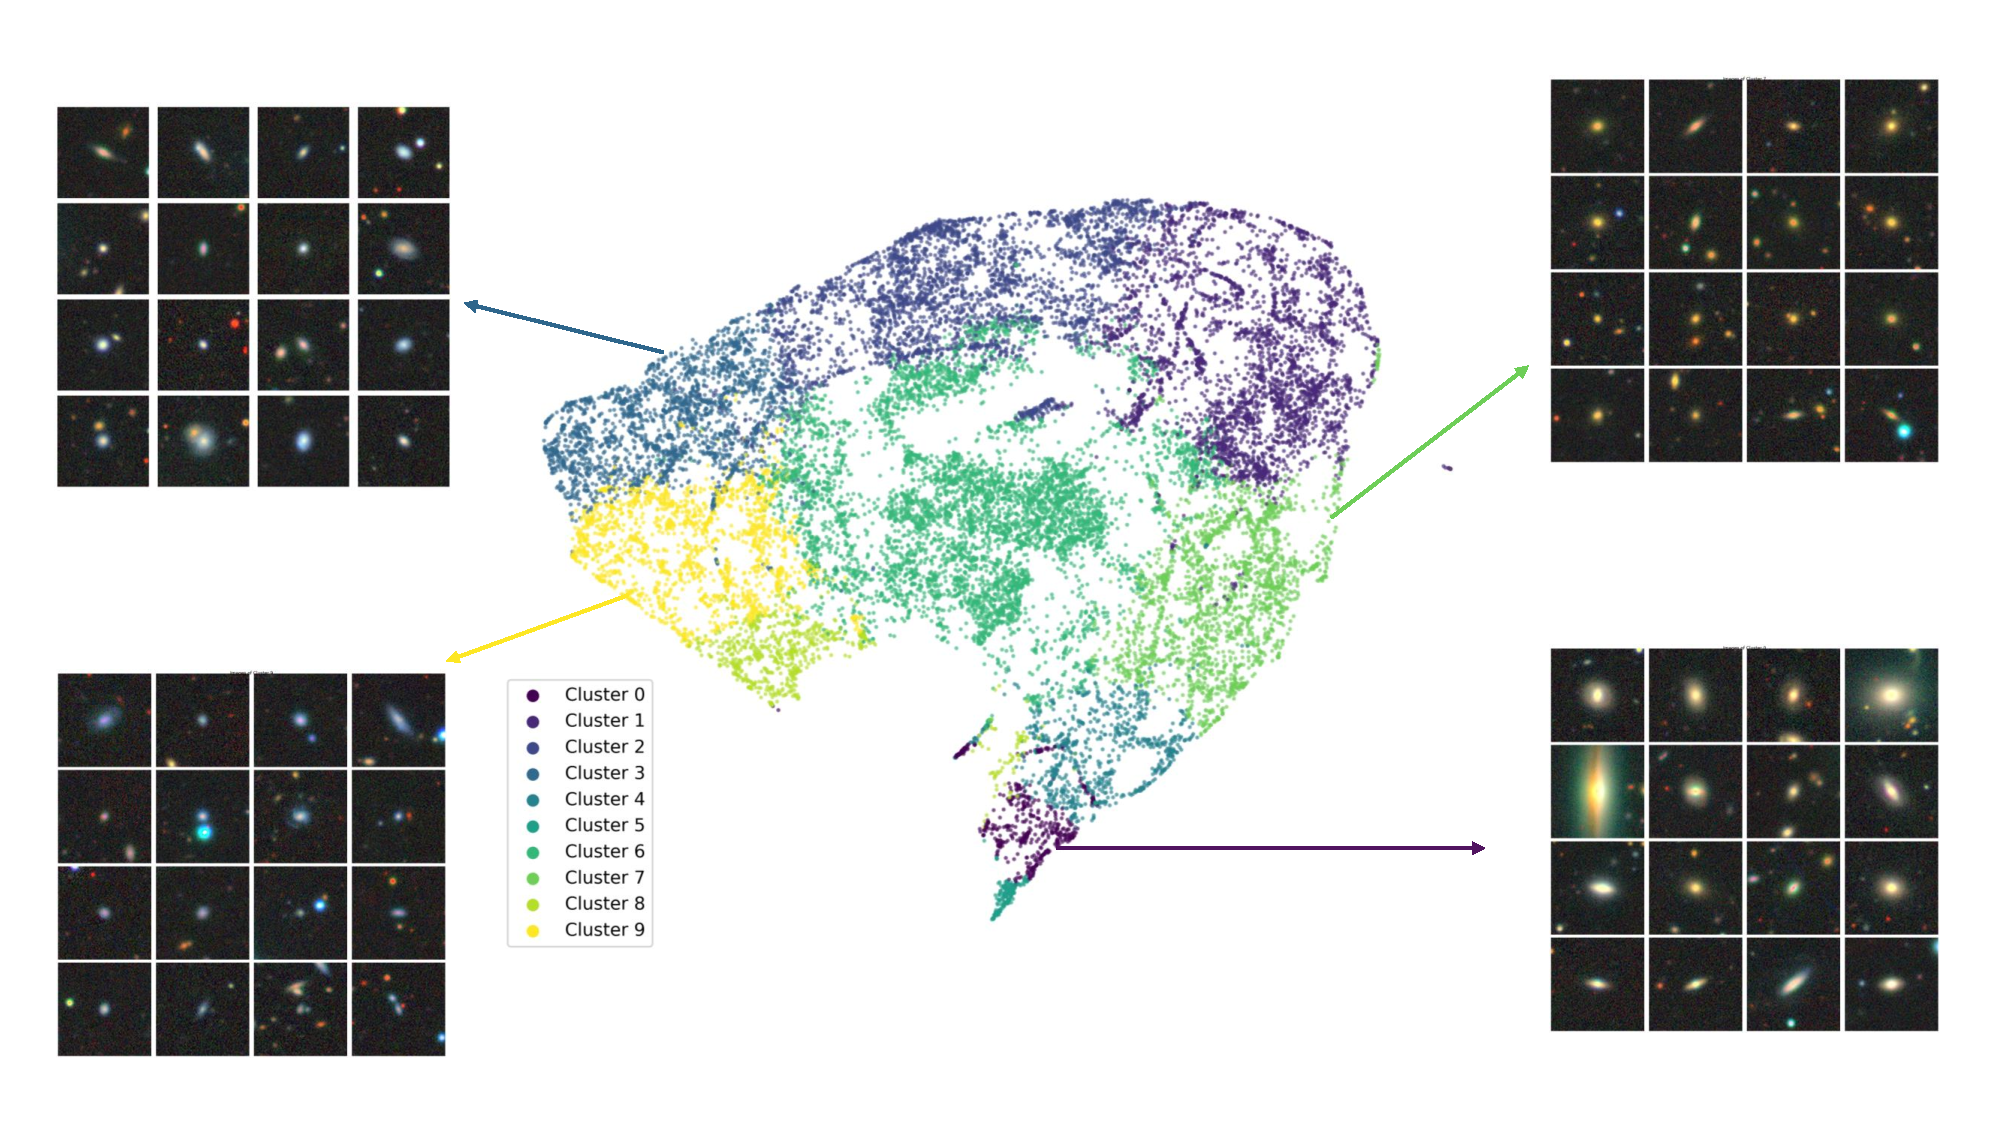
\includegraphics[width=1.15\textwidth]{../figures/umap_spectrum_annotated_images.pdf}
    \end{adjustbox}
    \caption{UMAP projection of the spectrum embeddings coloured by the $k$-Means clustering. The images of random samples from clusters [0,3,7,9] are shown in the four corners of this plot. The images are visually similar within their respective clusters.}
    \label{fig:annotated_images}

    
\end{figure}




\section{Conclusion}
% In this study, we successfully reproduced and extended the results of AstroCLIP—a cross-modal foundation model for galaxies that aligns image and spectrum embeddings in a shared latent space. First, we deployed two separate pre-trained single-modal encoders for galaxy images and spectra, which we modify to align the embeddings in a shared latent space. We then trained the cross-modal model under a InfoNCE constrastive loss to align the embeddings of the two modalities. Using the extracted embeddings, we demonstrated the model's ability to retrieve similar galaxies based on a query galaxy and predict physical properties such as redshift and stellar mass in a zero-shot regime. The latter is a key feature of the model, as it shows that the embeddings exhibit an emergent ability to structure themselves around physical properties, despite these not forming part of the training process.


% Despite using a smaller model than the original work, we achieved comparable results in all tasks. In addition to reproducing the original results, we extended the analysis by examining the structure of the embedding space using clustering algorithms and dimensionality reduction techniques. We demonstrate that the embeddings form clusters that are semantically separable in both modalities, which presents a concrete example of the model's ability to align the embeddings based on shared semantics. 


% Our results confirm the potential of cross-modal contrastive pre-training to achieve high-quality foundation models for astronomical data. This work opens up the avenue for the addition of other modalities in the same embedding space, such as photometry, multi-band images, or even text data. Ultimately, this constitutes one of the first applications of foundational models in science, a promising advent in the wider field of machine learning.

In this study, we successfully reproduced and extended the results of AstroCLIP—a cross-modal foundation model for galaxies that aligns image and spectrum embeddings in a shared latent space. Initially, we deployed two separate pre-trained single-modal encoders for galaxy images and spectra, which we modified to align the embeddings in a shared latent space. We then trained the cross-modal model using an InfoNCE contrastive loss to align the embeddings of the two modalities. Utilising the extracted embeddings, we demonstrated the model's capability to retrieve similar galaxies based on a query galaxy and to predict physical properties such as redshift and stellar mass in a zero-shot regime. This ability is a key feature of the model, indicating that the embeddings naturally structure themselves around physical properties, despite these not being part of the training process.

Despite employing a smaller model than the original work, we achieved comparable results in all tasks. Beyond reproducing the original results, we extended the analysis by examining the structure of the embedding space using clustering algorithms and dimensionality reduction techniques. We demonstrated that the embeddings form semantically separable clusters in both modalities, exemplifying the model's ability to align embeddings based on shared semantics.

Our results confirm the potential of cross-modal contrastive pre-training to achieve high-quality foundation models for astronomical data. This work opens the avenue for integrating additional modalities into the same embedding space, such as photometry, multi-band images, or even text data. Ultimately, this constitutes one of the first applications of foundation models in science, marking a promising advancement in the broader field of machine learning in science.



\newpage
\bibliographystyle{unsrt}
\bibliography{references.bib}

\newpage
\section*{Appendix}
\addcontentsline{toc}{section}{Appendix}

\subsection*{Use of Co-pilot}
Co-pilot was utilised in the following ways:
\begin{itemize}
    \item Autocompleting documentation for functions and for scripts.
    \item Understanding error messages with the `Explain this error' button next to the error message.
    \item Responding to general queries, especially LaTeX.
\end{itemize}

\noindent For example: \\
\noindent \textbf{Prompt1:} How do i put two images together in a single figure, horizontally next to each other, with the same caption, in latex? \\
\noindent \textbf{Answer1:} You can use the `subfigure' environment in LaTeX to put two images together in a single figure. Here is an example code snippet that puts two images next to each other with the same caption... \\
\noindent \textbf{Prompt2:} How can I change a function name and have it change throughout my workspace?
\noindent \textbf{Answer2:} In Visual Studio Code, you can use the ``Rename Symbol'' feature to change a function name throughout your workspace. Here are the steps:
\begin{enumerate}
    \item Place your cursor on the function name you want to change.
    \item Right-click the function name, and select ``Rename Symbol'' from the context menu. Alternatively, you can use the shortcut F2.
    \item Enter the new function name and press Enter.
\end{enumerate}
VS Code will automatically find and update all occurrences of the function name in your workspace. This includes not only the function definition but also all places where the function is called.

\end{document}